% v2-acmsmall-sample.tex, dated March 6 2012
% This is a sample file for ACM small trim journals
%
% Compilation using 'acmsmall.cls' - version 1.3 (March 2012), Aptara Inc.
% (c) 2010 Association for Computing Machinery (ACM)
%
% Questions/Suggestions/Feedback should be addressed to =>
% "acmtexsupport@aptaracorp.com".  Users can also go through the FAQs
% available on the journal's submission webpage.
%
% Steps to compile: latex, bibtex, latex latex
%
% For tracking purposes => this is v1.3 - March 2012

% \documentclass[prodmode,acmtecs]{acmsmall} % Aptara syntax
\documentclass[times]{cpeauth}

% Package to generate and customize Algorithm as per ACM style
\usepackage[colorlinks,bookmarksopen,bookmarksnumbered,citecolor=red,urlcolor=red]{hyperref}
\usepackage[linesnumbered]{algorithm2e}
\usepackage{tikz}
\usetikzlibrary{shapes,arrows}
\usepackage{fancyvrb}
\usepackage{paralist}
\usepackage{amsmath}
\usepackage{amsthm}
\usepackage{amssymb}
\usepackage{subfig}
\usepackage{listings}
\usepackage{xcolor}
\usepackage[inline]{enumitem}
\renewcommand{\algorithmcfname}{ALGORITHM}
\renewcommand\theFancyVerbLine{\small\arabic{FancyVerbLine}}
\captionsetup*[subfigure]{position=bottom}
\newenvironment{algo}{%
\renewenvironment{algocf}[1][h]{}{}%
\algorithm
}{%
\endalgorithm
}
\SetAlFnt{\small}
\SetAlCapFnt{\small}
\SetAlCapNameFnt{\small}
\SetAlCapHSkip{0pt}
\IncMargin{-\parindent}
\newsavebox{\verbbox}
\newsavebox{\verbboxx}
\newsavebox{\eone}
\newsavebox{\etwo}

\newtheorem{definition}{Definition}
% Metadata Information
% \acmVolume{}
% \acmNumber{}
% \acmArticle{}
% \acmYear{2014}
% \acmMonth{11}
\def\volumeyear{2016}

\lstdefinestyle{sysj}{ belowcaptionskip=1\baselineskip, breaklines=true,
  xleftmargin=\parindent, language=Java, showstringspaces=false,
  basicstyle=\small\ttfamily,
  keywordstyle=\bfseries\color{green!40!black},
  commentstyle=\itshape\color{purple!40!black},
  identifierstyle=\color{blue}, stringstyle=\color{orange},
  morekeywords={input,output,signal,channel,immediate,weak,sustain,send,receive,abort,await,emit,present,trap,pause,exit,wait_inbetween,wait_exact,wait_atleast,suspend},
  tabsize=2 }

% \linespread{0.99}

% Document starts
\begin{document}

% Page heads
\runningheads{A.~Malik~et al.}{Compiler assisted memory managements for
  hard real-time safety-critical applications}

% Title portion
\title{Compiler assisted memory management for safety-critical hard-real time 
  applications}

\author{Avinash~Malik~\corrauth,~HeeJong~Park,~Muhammad~Nadeem,~Zoran~Salcic}

\address{Department of Electrical and Computer Engineering, University
  of Auckland, New Zealand}

% \author{Avinash Malik
%   \affil{University of Auckland}
%   HeeJong Park
%   \affil{University of Auckland}
%   Muhammad Nadeem
%   \affil{University of Auckland}
%   Zoran Salcic
%   \affil{University of Auckland}
% }

\begin{abstract}

  Arguably the major hurdle in adoption of memory managed languages,
  such as Java, in the real-time systems community is the incorporation
  of garbage collection (GC) within the real-time application. It has
  recently been shown that the statically estimated worst case execution
  time (WCET) value of tasks invoking GC is pessimistic to such a great
  extent that incorporating them within the hard real-time scheduling
  framework is unfeasible. We develop a compiler assisted memory
  management technique for safety critical hard real-time applications
  developed in the synchronous subset of the formal globally
  asynchronous locally synchronous programming language called
  SystemJ. {\color{red} The SystemJ model of computation, clearly
    demarcates the state boundaries of the program, which in turn allows
    us to partition the heap, at compile time, into two distinct areas:
    (1) the memory area to hold objects that are live across state
    boundaries, called the permanent heap and (2) the memory area used
    to hold all other object, called the transient heap.} The new memory
  reclaim procedure is a simple pointer reset, which is guaranteed to
  complete within a bounded number of clock-cycles, thereby alleviating
  the need for large pessimistic WCET bounds obtained due to GC cycle
  times. Other than being amenable to formal verification and tight WCET
  analysis, results show that our proposed approach to memory management
  is approximately $3\times$ faster compared to standard real-time GC
  approaches.


\end{abstract}

% \category{D.3.4}{Processors}{Compilers}

% \terms{Compiler, Static Analysis, WCET, SystemJ, Garbage Collection}

\keywords{Compiler; Static Analysis; WCET; SystemJ; Garbage Collection}

% \acmformat{}
% At a minimum you need to supply the author names, year and a title.
% IMPORTANT:
% Full first names whenever they are known, surname last, followed by a period.
% In the case of two authors, 'and' is placed between them.
% In the case of three or more authors, the serial comma is used, that is, all author names
% except the last one but including the penultimate author's name are followed by a comma,
% and then 'and' is placed before the final author's name.
% If only first and middle initials are known, then each initial
% is followed by a period and they are separated by a space.
% The remaining information (journal title, volume, article number, date, etc.) is 'auto-generated'.


\corraddr{avinash.malik@auckland.ac.nz, Department of Electrical and
  Computer Engineering, University of Auckland, NZ}
\maketitle


% \section{Introduction and related work}
% \label{sec:introduction}

% With the advent of the Internet of Things (IoT) paradigm, the line
% between embedded real-time computing and standard desktop computing is
% blurring. As more sensors and actuators are connected to the embedded
% devices, the software code bases controlling these devices is only
% predicted to grow in complexity. In order to manage this inherent
% complexity, managed programming languages such as Java are being
% considered even for safety-critical and hard real-time
% systems~\cite{scj2013}. There are two main requirements that need to be
% satisfied when considering real-time and safety-critical systems: (1)
% respecting the environment specified space and time bounds and (2)
% guaranteeing functional correctness. Both these aspects have been
% studied in the research literature quite extensively for managed
% languages, especially
% Java~\cite{khav00,pizlo2008study,scj2013,puffitsch2013design}.

% For any given real-time system, \textit{Worst Case Execution Time}
% (WCET) of a task should be statically known so that real-time tasks can
% be scheduled to meet their individual
% deadlines~\cite{wilhelm08}. Computing WCET of a task programmed in a
% non-managed language such as `C' is a non-trivial task since detailed
% knowledge of hardware and interaction of the task and the underlying
% hardware needs to be known a-priori. Managed languages include a runtime
% environment with \textit{Just In Time} (JIT) compilation, which
% exacerbates the problem of computing the WCET of the task programmed in
% a managed language to such an extent as to render it unfeasible. In
% order to skirt this problem, researches (both academic and commercial)
% either perform ahead of time compilation of their Java
% programs~\cite{kalibera2011scheduling,pizlo2010schism} or use hardware
% implemented Java virtual machines~\cite{msch05}. In either case, the JIT
% compilation interference is no longer a problem in determining the WCET
% of the task. Instead, the main challenge now is to reconcile the memory
% allocation and garbage collection phases inherent to a managed language
% within the WCET static analysis framework.

% Many approaches to \textit{Real-time Garbage Collection} (RTGC) have
% been proposed, a good survey of RTGCs can be found
% in~\cite{pizlo2008study}. There are multiple requirements that a RTGC
% needs to satisfy. From the perspective of the real-time task, the main
% requirement is that: (1) the maximum blocking time for a GC should be
% bounded and (2) the number of \textit{times} a task may be interrupted
% by the GC should be bounded. From the perspective of the GC itself, one
% needs to statically guarantee that enough memory is available to keep
% pace with the memory allocations demanded by the real-time task.

% There are two principle approaches to integrating RTGCs within a
% real-time framework. The first approach pioneered by
% Henriksson~\cite{henriksson1998scheduling} requires one to schedule the
% GC real-time task as the lowest priority thread in slack time -- time
% between the completion of a task and its deadline to
% \textit{incrementally} collect garbage. The second approach is to use a
% periodically running GC as the highest priority task that preempts a
% real-time task and runs for a statically determined amount of
% time~\cite{bacon2003real} again incrementally collecting garbage. Both
% approaches require a preemptable real-time system. In the first approach
% the GC task might be preempted by a higher priority real-time task or an
% asynchronous event. In the second approach real-time tasks themselves
% need to be preempted by the GC task. This need for preemptability has
% two drastic consequences: (1) every access to heap allocated object
% needs to be guarded by read and write barriers, thereby increasing time
% for every heap access and also memory allocation itself, which in turn
% increases the task's WCET. (2) Automated functional verification of
% priority preemptive multi-tasking model via approaches such as
% model-checking~\cite{clarke-book00,khav00} is known to be intractable
% due to the exponential state space explosion problem. Thereby making it
% unfeasible to automatically verify such systems for functional
% correctness.

% The question then becomes: \textit{is programming real-time
%   safety-critical systems using a manged language just impractical?} In
% this paper we argue that a well thought out programming model along with
% compiler assisted memory management is not only a practical, but also an
% efficient approach to programming real-time and safety-critical systems
% using managed languages.

% The most important requirement is that the programming model of the
% managed language be formally verifiable or at least not be proactively
% hostile to formal verification. In our opinion a system that meets all
% its real-time deadlines, but is functionally incorrect is of little
% use. Hence, we prioritize functional correctness over real-time
% guarantees, although at the end, both requirements need to be
% satisfied. In order to adhere to this requirement we consider languages
% (within the real-time community) based on formal semantics that can be
% used for automated formal verification. Synchronous languages such as
% Esterel~\cite{gber931}, Lustre~\cite{nhal91}, Signal~\cite{pgue91} and
% \textit{Globally Asynchronous Locally Synchronous} (GALS) languages such
% as SystemJ~\cite{amal10} have been used to design large real-time and
% safety-critical
% systems~\cite{bouali1998xeve,ParkMNS14,LiMS14,malik12}. All these
% languages are not only based on formal mathematical semantics, but are
% also designed to be amenable to automated formal
% verification. Especially imperative languages Esterel and its derivation
% SystemJ have been designed to reduce the state space explosion problem
% exhibited during formal verification, by adhering to a very strict
% programmer specified state demarcation approach. The programming model
% for these languages can be described as follows: a synchronous program
% is quiescent until one or more events occur from the environment. Upon
% detecting the event, the synchronous program \textit{reacts}
% \textit{instantaneously} in zero time to respond to these inputs and
% becomes quiescent until the next input events arrive. The start and end
% of this reaction transition demarcate states of the program -- note that
% internal data updates do not lead to change in the program state thereby
% reducing the state space explosion problem. Furthermore, the reaction
% being logically in zero-time is by definition \textit{atomic} and always
% faster than the incoming input events, thereby guaranteeing that none of
% the incoming events are missed. In reality, the reaction does take
% sometime, all one needs to do is find out the \textit{Worst Case
%   Reaction Time} (WCRT) of any given synchronous program. This WCRT
% value determines the shortest inter-arrival time for input events from
% the environment.

% Many techniques exist for computing WCRT values for synchronous programs
% providing support for data-computation via a non-managed language
% (primarily `C'). A good review is available in~\cite{wilhelm08}. We are
% interested in the WCRT analysis of synchronous programs that support
% data computation via managed-languages like Java. The
% SystemJ~\cite{amal10} language provides the synchronous programming
% model as a subset along with Java driven data-computations, thereby
% mixing synchronous \textit{Model of Computation} (MoC) with a
% managed-language runtime environment. WCRT computation techniques have
% been developed for SystemJ~\cite{LiMS14}, but the authors do not state
% anything about the integration of the GC within this WCRT framework.

% The main \textbf{contribution} of this paper is to present a new memory
% management approach that is amicable to static WCRT analysis of
% synchronous programs intertwined with managed runtime environments for
% data-computation support. More concretely our contributions can be
% refined as follows:

% \begin{itemize}
% \item \textit{Programming model inspired memory organization}: In this
%   paper we present a new memory organization for Java and accompanying
%   static WCRT analysis based on the SystemJ MoC.
% \item \textit{Compiler supported memory allocation}: We present the
%   compiler transformations that are needed to statically guarantee the
%   \textit{Worst Case Memory Consumption} (WCMC) and \textit{allocation}.
% \item \textit{Real-time analyzable back-end code generation and garbage
%     collection}: We present a strategy to replace the object allocation
%   bytecodes with real-time analyzable alternatives. Furthermore, we also
%   present an object placement strategy, which allows for O(1) heap
%   accesses in all cases.
% \end{itemize}

\section{Introduction}
\label{sec:introduction}

Synchronous programming languages~\cite{berry92} allow building correct
by construction safety critical hard real-time applications, because
they are based on formal mathematical semantics, which allows the
compiler itself to act as a
model-checker~\cite{jagadeesan1995safety}. The major benefit of the
synchronous \textit{Model of Computation} (MoC) is that it is based on
the concept of a \textit{Finite State Machine} (FSM). Languages such as
Esterel~\cite{berry92} and its derivation SystemJ~\cite{amal10} have
been designed to reduce the state space explosion problem exhibited
during formal verification, by adhering to a very strict programmer
specified state demarcation approach. The programming model for these
languages can be described as follows: a synchronous program is
quiescent until one or more events occur from the environment. Upon
detecting the event, the synchronous program \textit{reacts}
\textit{instantaneously} in zero time to respond to these inputs and
becomes quiescent until the next input events arrive. The start and the
end of this reaction transition demarcate states of the program -- note
that internal data updates do not lead to change in the program state
thereby reducing the state space explosion problem. Furthermore, the
reaction being logically in zero-time is by definition \textit{atomic}
and always faster than the incoming input events, thereby guaranteeing
that none of the incoming events are missed. In reality, the reaction
does take time, one needs to find out the \textit{Worst Case Reaction
  Time} (WCRT) of any given synchronous program. This WCRT value
determines the shortest inter-arrival time for input events from the
environment.

Many techniques exist for computing WCRT values for synchronous programs
providing support for data-computation via a non-managed language
(primarily `C')~\cite{boldt07,proop10}. These WCRT estimation approaches
suffer from a fundamental problem; they cannot incorporate complex
data-computations within the WCRT analysis framework, because of the
many undefined behaviors, type unsafety and the general lack of formal
operational semantics inherent to low-level non-managed
languages. Hence, in this paper we are interested in the WCRT analysis
of synchronous programs that support data computation via
managed-languages like Java, which provides a well defined operational
semantics. The key hurdle to the adoption of managed languages in the
safety critical hard real-time application domain is \textit{Garbage
  Collection} (GC) for automatic memory management, since worst case
execution time estimates for real-time tasks with GC are very
pessimistic~\cite{puffitsch2013design}.

% On the one hand GC guarantees no memory leaks, thereby providing
% functional safety, but on the other hand, it has been
% shown~\cite{puffitsch2013design} that using even a state of the art
% real-time GC results in very pessimistic worst case execution time
% estimates for real-time tasks.,~\footnote{The worst case execution time
%   was estimated to be in seconds due to the GC, but the observed time
%   was in milli-seconds.} compared to the observed task execution times,
% thereby rendering worst case execution/reaction time analysis unfeasible
% in the general case with a GC.

The main \textbf{contribution} presented in this paper is a new memory
management approach that is amicable to static WCRT analysis of
synchronous programs intertwined with managed runtime environments for
data-computation. More concretely our contributions can be refined as
follows:

\begin{itemize}
\item \textit{Programming model inspired memory organization}: In this
  paper we present a new memory organization for Java and an
  accompanying static WCRT analysis based on the synchronous MoC.
\item \textit{Compiler supported memory allocation}: We present the
  compiler transformations that are needed to statically guarantee the
  \textit{Worst Case Memory Consumption} (WCMC) and \textit{allocation}.
\item \textit{Real-time analyzable back-end code generation and garbage
    collection}: We present a strategy to replace the object allocation
  bytecodes with real-time analyzable alternatives. Furthermore, we also
  present an object placement strategy, which allows for O(1) heap
  accesses in all cases.
\end{itemize}

We use the SystemJ~\cite{amal10} programming language, because it
provides the synchronous MoC as a subset along with Java data-driven
computation support. Furthermore, there exist efficient and real-time
analyzable execution architectures~\cite{nadeem2011rjop} and WCRT
analysis tools~\cite{LiMS14} that support subset of SystemJ programs;
those without GC invocation.


% Local Variables:
% mode: latex
% TeX-master: "jgc"
% End:


The rest of the paper is arranged as follows:
Section~\ref{sec:preliminaries} gives the preliminary information needed
to read the rest of the paper. Section~\ref{sec:motiv-example-curr}
gives the motivating example to explain the SystemJ language and its
WCRT analysis. Section~\ref{sec:new-memory-model} gives the overview of
the new memory management scheme. Section~\ref{sec:comp-analys-stat}
describes the main data-flow analysis algorithm used for compile time
memory allocation. Section~\ref{sec:prod-back-code} explains the
back-end code generation
procedure. Section~\ref{sec:experimental-results} gives the quantitative
results comparing the presented technique with real-time garbage
collection alternatives. Section~\ref{sec:related-work} gives a thorough
comparison of the work described in this paper with current state of the
art.  Finally, we conclude in Section~\ref{sec:concl-future-work}.

\section{Preliminaries}
\label{sec:preliminaries}

Before we present the key contributions of the paper, we dedicate this
section to the description of the preliminary information needed by the
reader.

\subsection{The SystemJ programming language}
\label{sec:syst-progr-lang}

SystemJ~\cite{amal10} extends the Java programming language by
introducing both synchronous and asynchronous concurrency. SystemJ
integrates the synchronous essence of the Esterel~\cite{berry92}
language with the asynchronous concurrency of \textit{Communicating
  Sequential Processes} (CSP)~\cite{choa78}. SystemJ is grounded on
rigorous mathematical semantics and thus is amenable to formal
verification. We will use the graphical representation of a SystemJ
program in Figure~\ref{fig:3a} for explaining the SystemJ MoC. On the
top level, a SystemJ program comprises a set of clock-domains (CD1, CD2,
CD3) executing asynchronously. Each clock-domain is a composition of one
or more synchronous parallel reactions (Reaction11, Reaction12, etc),
which are executed in lock-step with the logical tick of the
clock-domain. Reactions within the same clock-domain exploit synchronous
broadcast mechanism on objects called signals to communicate with each
other. Reactions can themselves be composed of more synchronous parallel
reactions, thereby forming a hierarchy. Finally, every reaction in the
clock-domain communicates with the environment through a set of
interface input and output signals. At the beginning of each
clock-domain tick the input signals are captured, a reaction function
processes these input signals and emits the output signals. These output
signals are presented to the environment at the end of the clock-domain
tick. Inter-clock-domain communication is achieved by implementing CSP
style rendezvous mechanism through point-to-point unidirectional
channels. A complete list of SystemJ kernel statements is shown in
Figure~\ref{fig:1}. {\color{red} The compile time memory allocation
  strategy described in this paper is applicable to each clock-domain
  individually and hence, in the rest of the paper we concentrate only
  on a single clock-domain.  }

In this work we are only interested in the synchronous subset of
SystemJ, i.e., a single clock-domain.

\begin{figure}[t!]
  \centering
  \[
  \begin{scriptsize}
    \begin{array}[h!]{|c|c|}
      \hline
      \mathbf{noop}  & \mathrm{do\ nothing}\\
      \hline
      \mathbf{pause}  & \mathrm{complete\ a\ logical\ tick}\\
      \hline
      \mathbf{[input] [output] [type] signal\ \sigma} &  \mathrm{declare\ signal\ \sigma} \\
      \hline
      \mathbf{emit\ \sigma [value]} &  \mathrm{broadcast\ signal\ \sigma} \\
      \hline
      \mathbf{abort\ (\sigma)\ s} &  \mathrm{preempt\ statement\ s\ if\ \sigma\ is\ true} \\
      \hline
      \mathbf{suspend\ (\sigma)\ s} &  \mathrm{suspend\ statement\ s\ for\
                                      one\ tick\ if\ \sigma\ is\ true} \\
      \hline
      \mathbf{present\ (\sigma)\ s1\ else\ s2} &  \mathrm{do\ s1\ if\
                                                 \sigma\ is\ true\ else\ do\ s2} \\
      \hline
      \mathbf{s1;s2} &  \mathrm{do\ s1\ and\ then\ s2} \\
      \hline
      \mathbf{s1||s2} &  \mathrm{do\ s1\ and\ s2\ in\ lockstep\ parallel} \\
      \hline
      \mathbf{while(true)\ s} &  \mathrm{do\ s\ forever} \\
      \hline
      \mathbf{jterm} &  \mathrm{Java\ data\ term} \\
      \hline
    \end{array}
  \end{scriptsize}
  \]
  \caption{Syntax of the synchronous subset of the SystemJ language}
  \label{fig:1}
\end{figure}

Signals are the primary means of communication between reactions of a
clock-domain and between a clock-domain and its environment. A signal in
SystemJ can be typed or untyped. Every untyped signal in SystemJ is
called a pure signal and only consists of a Boolean status, which can be
set to \texttt{true} or \texttt{false} via signal emission. A typed
signal is called a valued signal, and consists of a value (of any Java
data-type) in addition to the status. The value of a typed signal can
also be set, optionally, via the $\mathbf{emit}$ statement. Once
emitted, the status of a signal is \texttt{true} only for a single tick,
but the value of a signal is persistent over ticks. Emission of a
signal, broadcasts it across all reactions within the
clock-domain. Moreover, the updated status and value of the signal, upon
emission, is only visible in the next tick.

SystemJ provides mechanisms to describe reactivity via statements such
as $\mathbf{present}$, $\mathbf{abort}$, and $\mathbf{suspend}$, which
change the control-flow of a SystemJ program depending upon signal
statuses. The control-flow of a program can also be altered via standard
Java conditional constructs. Synchronous (lock-step) parallel execution
of reactions within a SystemJ program is captured using the synchronous
parallel ($||$) operator~\footnote{Standard Java threading model is not
  allowed within SystemJ. Instead, synchronous and asynchronous parallel
  operators need to be used.}. Furthermore, shared variable
communication between synchronous parallel reactions is not allowed in
SystemJ. The shared memory communication model is replaced by the signal
emission based communication mechanism. State boundaries are demarcated
explicitly by programmers using the $\mathbf{pause}$ construct. Finally,
there are two types of loops in SystemJ: temporal; consisting of a
$\mathbf{pause}$ statement, loops that execute forever and bounded
data-loops like in standard Java.

\subsection{The real-time execution architecture}
\label{sec:real-time-execution}

Every static WCRT analysis technique needs intimate knowledge of the
hardware that executes the program. For our purpose, we choose a
multi-core time predictable execution platform called
\textit{Tandem-Java Optimized Processor}
(TP-JOP)~\cite{DBLP:journals/tecs/SalcicM13,nadeem2011rjop}. There are
two main reasons we chose this processor architecture: (1) efficiency --
it has been shown previously that the TP-JOP processor architecture is
much more efficient for executing SystemJ programs compared to general
purpose Java processors~\cite{ParkMNS14} and (2) there already exists
tools for statically estimating tight WCRT bounds for synchronous
SystemJ programs executing on the TP-JOP architecture~\cite{LiMS14}.

\begin{figure}[t!]
  \centering
  \subfloat[A graphical representation of a SystemJ program]{
    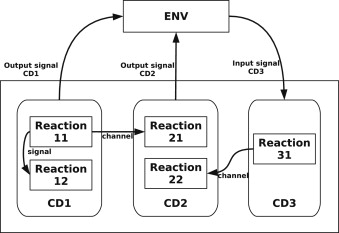
\includegraphics[scale=0.7]{gsysj.jpg}
    \label{fig:3a}
  }
  \qquad
  \subfloat[Overview of the TP-JOP architecture]{
    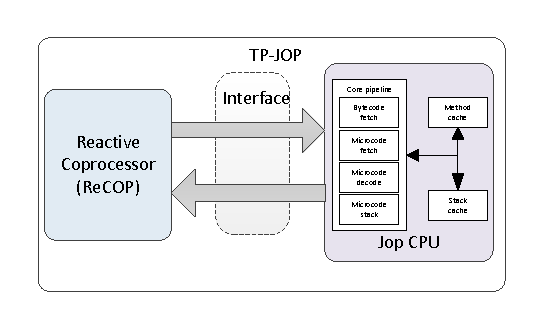
\includegraphics[scale=0.8]{tpjop}
    \label{fig:3b}
  }
  \caption{A generic SystemJ program and its execution architecture}
  \label{fig:3}
\end{figure}

Figure~\ref{fig:3b} gives an overview of the TP-JOP architecture. The
architecture consists of two time predictable cores. The first core is
termed \textit{Reactive Co-processor} (ReCOP) that executes the control
flow instructions of a SystemJ program. The Java data computations are
dispatched to the JOP core on a as needed basis by the ReCOP. ReCOP has
a multi-cycle data-path, and each native ReCOP instruction is executed
in 3 clock cycles. ReCOP core uses a single small private memory for
both: data and program.

The JOP~\cite{msho03} core is a hardware implementation of the Java
Virtual Machine (JVM). The JOP core is a four stage pipelined
processor. Every Java bytecode is translated into one or more
microcodes, which are the native instructions of the JOP processor. The
JOP pipeline has been designed to execute each microcode in one clock
cycle and is guaranteed to be stall free. Furthermore, to guarantee time
predictability, a novel cache architecture is implemented in JOP. There
are two caches in JOP. The first is the stack cache that acts as a
replacement for the data cache found in general purpose processors. The
second is the method cache that acts as a replacement for program
cache. A complete Java method is loaded into the method cache before
execution and hence, there are only two program points: the
\textit{invoke} and the \textit{return} bytecodes that can lead to a
method cache miss, which can be accounted for in the static WCRT
analysis procedure with ease. Finally, the interface connecting the
ReCOP and JOP has single clock cycle latency as described
in~\cite{DBLP:journals/tecs/SalcicM13}.

The overall program execution on the TP-JOP architecture proceeds as
follows: the ReCOP leads the program execution since it executes the
control-flow graph of the SystemJ program. When a data computation node
is encountered, a call is dispatched to the JOP core with a method
ID. Upon dispatch, the ReCOP itself stops processing further
instructions until a result is returned from JOP. The JOP core polls
continuously for an incoming request from ReCOP. Once a request is
received, JOP decodes the method ID and loads the method into the method
cache. Once loaded, the requested method is executed and upon completion
of execution, the result is returned back to ReCOP.

\section{Statically estimating WCRT of SystemJ clock-domains}
\label{sec:motiv-example-curr}

% We present a motivating example of fruit sorter control system for
% elucidating the synchronous semantics of the SystemJ language and
% explaining the approach employed for static WCRT analysis of SystemJ
% synchronous clock-domains.

% import fruitsorter.*;
% //Declare the SystemJ clock-domain 
% //with its interface signals
% FruitSorterController(
%  input signal NEW_ITEM,ITEM_READY,REACHED_HOME;
%  input signal REACHED_LEFT,REACHED_RIGHT;
%  output signal PICK_TO_LEFT,PICK_TO_RIGHT, 
%   MOVE_HOME;
% )->{
%  Image signal Picture; 
%  String signal Item_Type;
%  while(true) {
%   {//R1: take a picture of item using Camera
%    await (NEW_ITEM);//from Sensor1
%    emit Picture(Camera.takepicture());\label[fig:4l1]
%   }
%   ||
%   {//R2: recognize and emit image type
%    await (Picture);
%    emit Item_Type(
%     Process_Image.get_item_type (
%     (Image)#Picture));
%   }
%   ||
%   {//R3: Mechanical arm controller logic
%    await(REACHED_HOME); //R4
%    ||
%    await(Item_Type); //R5
%    ||
%    await(ITEM_READY); //R6
%    if ((String)#Item_Type.equals(``apple''))
%    {//put item into apple bin
%     emit PICK_TO_LEFT;
%     await(REACHED_LEFT);
%    } else {
%     //put item into pear bin
%     emit PICK_TO_RIGHT;
%     await(REACHED_RIGHT);
%    }
%    emit MOVE_HOME;
%   }
%   pause;
%  }
% }
\begin{lrbox}{\verbboxx}
  \begin{minipage}[b]{0.5\linewidth}
    \begin{scriptsize}
      
\begin{Verbatim}[numbers=left,commandchars=\\\[\]]
SysJ_Example(
  output signal OUTPUT; \label[ex1:l1o]
  input Integer signal INPUT_A; \label[ex1:l2]
  input Integer signal INPUT_B; \label[ex1:l3]
 )->{
 {\label[ex1:r1s]
   int count_a = 0;
   while(true){\label[ex1:l1]
     present (INPUT_A) {\label[ex1:cA]
       if (#INPUT_A == 0)\label[ex1:d1s]
       //...data computation
       else ++count_a;\label[ex1:d1e]
     } else --count_a; \label[ex1:d2]
     pause;\label[ex1:p1]
   }
 }\label[ex1:r1e]
 || \label[ex1:sc]
 {\label[ex1:r2s]
   int count_b = 0;
   while(true){
     present(INPUT_B)\label[ex1:cB]
       ++count_b; \label[ex1:d3]
     else emit OUTPUT;
     pause;
   }
 }\label[ex1:r2e]
}
\end{Verbatim}
    \end{scriptsize}
  \end{minipage}
\end{lrbox}

\begin{figure}[b!]
  \centering
  \subfloat[Example synchronous SystemJ clock-domain]{
    \scalebox{0.65}{\usebox{\verbboxx}}
    \label{fig:4}}
  \subfloat[GRC of the SystemJ clock-domain in
  Figure~\ref{fig:4}] 
  {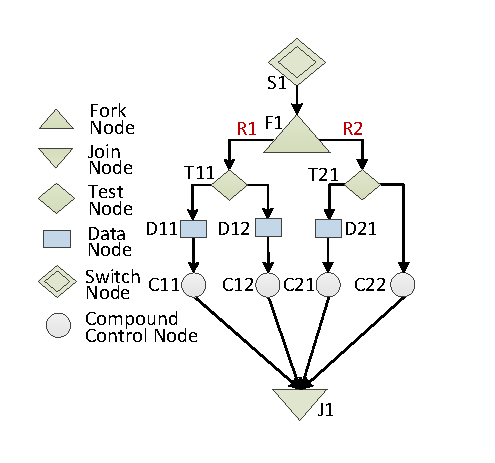
\includegraphics[scale=0.6]{grc}\label{fig:2a}}
  \subfloat[Uppaal representation of GRC] 
  {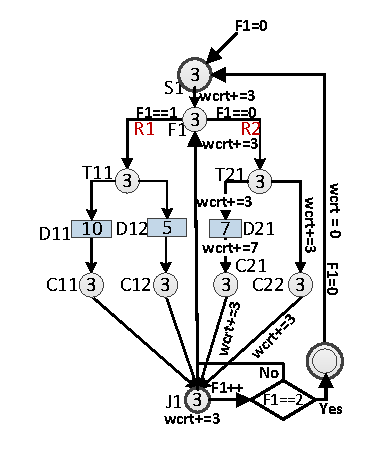
\includegraphics[scale=0.7]{ugrc}\label{fig:2b}}
  \caption{Example SystemJ program with its GRC and Uppaal
    representations}
  \label{fig:2}
\end{figure}

% As shown in Figure~\ref{fig:2a}, the fruit sorter consists of a fruit
% loader, a conveyor belt, a mechanical arm, a camera and two sensors.
% The fruit loader places fruit items on the left end of the conveyor belt
% at a constant speed and the conveyor belt moves from left to right
% carrying fruit items. The pictorial representation of SystemJ
% clock-domain controlling the fruit sorter is also shown in
% Figure~\ref{fig:2a}. The clock-domain contains six reactions (from R1 to
% R6). The presence of a fruit item loaded at the left end of the conveyor
% belt is detected by Sensor 1 that produces an input signal
% \texttt{NEW\_ITEM} to R1. Upon arrival of this signal, a picture of the
% fruit is taken in R1 and analyzed to determine the type of the item
% (either apple or pear in this example) in R2. This analysis is then used
% to sort the fruit into the appropriate bin via a Mechanical sorting arm.

% Reactions R4-R6 wait for three input signals in parallel before
% performing actual sorting operation: (1) the \texttt{Item\_Type} signal
% from R2, (2) \texttt{ITEM\_READY} signal produced by Sensor 2,
% indicating that a fruit item is present at the right end of the conveyor
% belt and ready to be sorted and (3) \texttt{REACHED\_HOME} signal
% indicating the mechanical arm has completed the previous sorting
% procedure. Upon the arrival of all these three input signals, R3 emits
% \texttt{PICK\_TO\_LEFT} or \texttt{PICK\_TO\_RIGHT} signal to indicate
% to the mechanical arm to pick the item and move to the correct bin, R3
% then awaits for the \texttt{REACHED\_LEFT} or \texttt{REACHED\_RIGHT}
% signal indicating that the mechanical arm has reached atop the correct
% bin and dropped the item, then \texttt{MOVE\_HOME} signal is emitted to
% bring the mechanical arm back to its initial position.


% \begin{figure}[t!]
%   \centering
%   \caption{Fruit sorter controller clock-domain implementation in
%   SystemJ}
%   \label{fig:4}
% \end{figure}

% The SystemJ clock-domain implementing this control logic is shown in
% Figure~\ref{fig:4}. There are two hard real-time requirements for the
% control logic: (1) the time spent on item recognition should be shorter
% than the inter-arrival time of the incoming input signal
% \texttt{NEW\_ITEM}, else, the type of the fruit cannot be recognized and
% (2) the mechanical arm should sort items faster than the inter-arrival
% time of the input signal \texttt{ITEM\_READY}, else, the fruit will not
% be placed into the bin and will drop off the conveyor belt. These timing
% constraints essentially mean that the WCRT for synchronous fruit sort
% controller should be shorter than the inter-arrival time of input
% events.

% \subsection{Static WCRT analysis of a SystemJ synchronous clock-domain}
% \label{sec:static-wcrt-analysis}

% In order to guarantee the timing requirements of the fruit sorter
% control logic we need to statically determine the WCRT of the fruit
% sorter controller clock-domain. The static analysis performed to
% estimate the WCRT of any synchronous SystemJ clock-domain is described
% in~\cite{LiMS14}. Here in we give a brief overview of the procedure.

% \begin{lrbox}{\verbbox}
%   \begin{minipage}[b]{0.5\linewidth}
%     \begin{Verbatim}[numbers=left,commandchars=+\[\]]
% public class FruitSorterController {
%  //signal NEW_ITEM declaration
%  private static Signal NEW_ITEM;
%  ...//other signal and object declarations
%  public static void init () {
%   NEW_ITEM = new Signal();
%  }
%  public static void main(String args[]){
%   init();
%   while(true){
%    //poll on the method call request from ReCOP
%    int methodnum = Native.rd(Const.METHOD_NUM);
%    switch(methodnum){
%     case 0: ...
%     ...
%     //Call method representing action node
%     //in GRC
%     case 24: Native.wr(RESULT_REG,
%     MethodCall24_0());
%    }
%   }
%  }
%  private static boolean MethodCall24_0(){+label[fig:5bl1]
%    // Compiled from Figure +ref[fig:4], line +ref[fig:4l1]
%    imm_thread_4 = Camera.takepicture();
%    //signal value emission
%    picture_1.setValue(imm_thread_4);+label[fig:5bl2]
%    return false;
%  }
% }
%     \end{Verbatim}
%   \end{minipage}
% \end{lrbox}

% \begin{figure}[t!]
%   \centering 

%   \subfloat[The GRC intermediate format for the fruit sorter controller
%   clock-domain]{
%     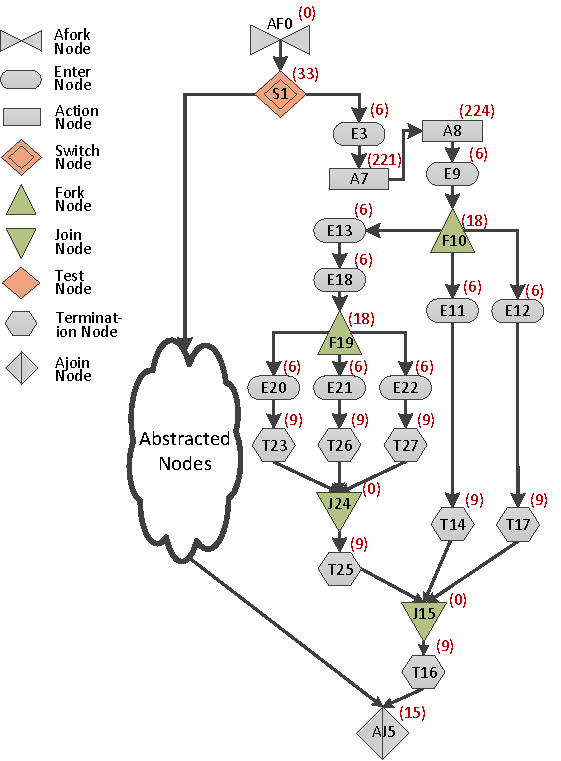
\includegraphics[scale=0.6]{agrc}
%     \label{fig:5a}
%   }
%   \qquad
%   \subfloat[The generated back-end Java code for JOP]{
%     \scalebox{0.7}{\usebox{\verbbox}\label{fig:5b}}
%   }
%   \caption{GRC intermediate format and generated back-end code for
%     TP-JOP architecture}
%   \label{fig:5}
% \end{figure}

In this section we use a pedagogical SystemJ synchronous program to
describe the static analysis technique used to estimate the WCRT of
SystemJ clock-domains. The WCRT estimation technique is not the main
contribution of this paper and hence, we only give a brief overview of
the approach. The reader is referred to~\cite{LiMS14} for a more
detailed description of the technique.

Figure~\ref{fig:4} shows a simple SystemJ synchronous program. The
program declares two input signals (lines~\ref{ex1:l2} and~\ref{ex1:l3})
that are used to capture events generated from the external environment
and one output signal (line~\ref{ex1:l1o}) used to produce events back
to the external environment. Two concurrent reactions
(lines~\ref{ex1:r1s}-\ref{ex1:r1e} and~\ref{ex1:r2s}-\ref{ex1:r2e})
execute in lock-step parallel, composed using the synchronous parallel
operator ($||$) on line~\ref{ex1:sc}. Reaction R1 checks for an incoming
event on the input signal \texttt{INPUT\_A} (line~\ref{ex1:cA}). If an
event is detected, a counter is incremented, else, it is
decremented. This logic is carried out forever using an infinite loop
(line~\ref{ex1:l1}). The pause construct (line~\ref{ex1:p1}) explicitly
demarcates the end of program transition. Similarly, a counter
\texttt{count\_b} is incremented upon reception of an event on signal
\texttt{INPUT\_B} in reaction R2, else signal \texttt{OUTPUT} is emitted
to the external environment.

\subsection{GRC representation of the clock-domain}
\label{sec:grc-repr-clock}

% Every SystemJ clock-domain is compiled into an intermediate format
% called the \textit{Asynchronous Graph Code} (GRC)~\cite{amal10}. The
% GRC format of the fruit sorter controller clock-domain is shown in
% Figure~\ref{fig:5a}. The GRC intermediate format is akin to the
% control-flow graph of a program developed in a standard programming
% language, except that it also encodes parallelism and state
% representation specific to SystemJ. 

The semantics of a synchronous program described in SystemJ is captured
using an intermediate format called \textit{GRaph Code}
(GRC)~\cite{amal10}. The GRC is a directed acyclic graph that explicitly
describes the control flow of a synchronous program through primitive
nodes.

\begin{definition} \textit{Clock-domain transition (or tick)}: A single
  clock-domain transition also called a clock-domain tick is a
  \underline{single} traversal of the GRC from the source node (node
  with no incoming edges) to the sink node (node with no outgoing
  edges).
\end{definition}

Java statements in SystemJ are represented as data nodes. State encoding
and selection are captured with enter and switch nodes,
respectively. Present statements are denoted by test nodes. Concurrency
embodied by parallel reactions is delineated using fork and join
nodes. A fork node spawns parallel reactions, while a join node
instructs that the parent reaction waits until all child reactions
finish processing, which results in synchronized lock-step
execution. Each node in the GRC is a schedulable unit, which can be
either: (a) a java data node (JDN) representing data-driven computation
implemented as Java methods, or (b) a control node (CN) representing all
nodes other than JDNs, implemented on the ReCOP. All control nodes
between two data nodes are grouped together to form a single compound
control node in order to simplify the GRC. The GRC of the SystemJ
program shown in Figure~\ref{fig:4} is depicted in
Figure~\ref{fig:2a}. The fork node F1 creates two parallel reactions R1
and R2 at the start of the program. The present statements
(lines~\ref{ex1:cA} and~\ref{ex1:cB}) are represented as nodes T11 and
T21, respectively in the GRC. The Java data computations at
lines~\ref{ex1:d1s}-\ref{ex1:d1e},~\ref{ex1:d2}, and~\ref{ex1:d3} are
represented as nodes D11, D12, and D22, respectively. Finally, the
infinite loops are simply infinite executions of the GRC


% Every GRC starts with the \texttt{AforkNode} representing forking of
% multiple clock-domains, in case of the fruit sorter controller, a single
% clock-domain is forked. The \texttt{Enter} and \texttt{Switch} nodes
% together encode the state information. The \texttt{Enter} node sets the
% value of a \texttt{Switch} node in any given program transition. The
% \texttt{Switch} node then uses this value in the next transition to
% choose a branch for execution. The synchronous parallelism is captured
% using \texttt{Fork} and \texttt{Join} nodes. Every \texttt{Fork} node
% forks multiple synchronous parallel reactions for execution, which are
% then synchronized to the clock-domain tick at the \texttt{Join}
% node. The signal emissions and Java data-computations are captured
% within the \texttt{Action} nodes. The \texttt{Test} nodes are used for
% branching on signal statuses. Finally, \texttt{Terminate} nodes, capture
% the termination context of the currently executing clock-domain
% transition. A program is considered alive and ready to execute the next
% tick if the GRC pass terminates with value of 1, a value of 0 means
% completion of the program and all further program transitions are
% disabled.

\subsection{WCRT estimation using the Uppaal model-checker}
\label{sec:wcrt-estim-using}

Finding the WCRT of a SystemJ clock-domain is equivalent to finding the
longest execution path from source node to the sink node in the
GRC. Finding this longest path is non-trivial, because of concurrent
execution of the synchronous parallel reactions, the execution of
different control branches depending upon the incoming input events from
the external environment, and the state decoding within the switch
nodes. {\color{red} There are a plethora of static WCRT estimation
  techniques in the research
  literature~\cite{proop10,bbec10,roop09,sand11,theiling2000fast}. In
  this paper we describe one of the original techniques based on
  model-checking. Any other static WCRT estimation technique can be used
  in our compiler framework. We use the Uppaal~\cite{gbeh04}
  model-checker to perform an exhaustive state space exploration of the
  GRC, in the process, emulating the execution of the GRC on the TP-JOP
  architecture to find the WCRT of the SystemJ clock-domain. The
  exhaustive search space carried out by the Uppaal model-checker gives
  WCRT estimates, for SystemJ programs, that are on average
  $\approx 30\%$ tighter than those obtained by other
  approaches~\cite{LiMS14}.  } There are three steps involved in finding
the WCRT of a clock-domain using Uppaal:

\begin{enumerate}
\item \textit{Annotating the GRC nodes with \textit{Worst Case Execution
      Time} (WCET) values}: The GRC is annotated with timing information
  in order to compute the WCRT of the clock-domain. All CNs are executed
  on the ReCOP and hence, their timing information can be easily
  computed, as all native ReCOP instructions take 3 clock cycles to
  execute. The JDNs are dispatched, encapsulated within individual Java
  methods, for execution on JOP. One needs to compute the \textit{Worst
    Case Execution Time} (WCET) for each of these JDNs, using the JOP
  provided worst case analysis tool (WCA)~\cite{msch05}. The computed
  worst case execution times for both: CNs and JDNs are back annotated
  onto the GRC. The numerical annotations on the nodes in
  Figure~\ref{fig:2b} show these back annotated WCETs.

\item \textit{Translating the GRC into an Uppaal timed automaton}:
  Figure~\ref{fig:2b} shows the GRC of the pedagogical SystemJ
  clock-domain captured as a \textit{Timed Automaton} (TA) in
  Uppaal. All nodes and edges in the GRC are mapped as locations and
  edges in the TA. Given the TP-JOP architecture, we know that all
  control nodes are executed only on a single ReCOP. Consequently, all
  synchronous parallel reactions can only be executed sequentially. In
  order to enforce this sequential execution of the synchronous parallel
  reactions, we introduce extra integer type variables for each fork
  node, e.g., $F1$ in Figure~\ref{fig:2b}. These fork variables are
  initialized to 0. Furthermore, a back-edge is added from the
  corresponding join node to the fork node, which increments the fork
  variable ($F1$ in Figure~\ref{fig:2b}).  Upon reaching the join-node,
  during state space exploration, the back-edge is taken as long as the
  value of the fork variable is not equal to the number of synchronous
  parallel reactions (2 in Figure~\ref{fig:2b}). Thereby, guaranteeing
  sequential execution of the synchronous parallel reactions. An integer
  type variable $wcrt$, is added to the TA~\footnote{We use an integer
    variable instead of a clock variable in Uppaal, because we are
    computing the worst case reaction time in terms of clock cycles of
    the program, not in seconds.}. No additions are needed for the test
  nodes, since the model-checker implicitly backtracks and explores all
  branches of the test nodes. The $wcrt$ variable is incremented by the
  WCET of individual nodes in the TA at every edge.  Finally, to emulate
  the execution of multiple ticks, and consequently explore all branches
  of the switch nodes, a back-edge is also added from a dummy sink node
  back to the source node. The $wcrt$ and fork values are reset upon
  execution of this back-edge.

\item \textit{Using a \textit{Computational Tree Logic} (CTL) property
    to obtain the WCRT}: We model the WCRT estimation problem as
  verifying a CTL property in the Uppaal model-checker. The WCRT value
  lies in the bounded range denoted by $[WCRT_{lb}, WCRT_{ub}]$.
  $WCRT_{ub}$ is a safe upper bound on WCRT obtained by applying
  Max-Plus algebra on the GRC, which is essentially summing up the
  maximum tick execution time of every reaction in the
  clock-domain. Similarly, we calculate a lower-bound of WCRT, termed
  $WCRT_{lb}$, by summing up the minimum tick execution time of every
  reaction in the clock-domain. After translating GRC to TA, we check
  the validity of the WCRT estimate of the clock-domain, termed
  $WCRT_{est}$, between $[WCRT_{lb}, WCRT_{ub}]$ by verifying a CTL
  property upon the TA using the Uppaal model checker. The CTL property
  is written as $A[](wcrt \leq WCRT_{est})$, meaning that the value of
  $wcrt$ variable in the TA is less or equal to the $WCRT_{est}$ for
  every path in the TA starting from the initial location. Upon
  violation of this property we are guaranteed that we have found the
  tightest $WCRT_{est}$ value.
\end{enumerate}

% Once, annotated, the GRC model is further translated into a labeled
% transition system (LTS) for input into the Uppaal
% model-checker~\cite{gbeh04}. A computational tree logic
% (CTL)~\cite{clarke-book00} property of the form:
% \mbox{$A[] (wcrt < num)$}, which, put informally, asks the
% model-checker to \textit{verify} that there exists no path in the
% program, from the \texttt{AforkNode} to the \texttt{AjoinNode}, with a
% wcrt value greater than some number $num$. The integer value $wcrt$ is
% incremented by the model-checker by the WCET value of the GRC node
% encountered.

% This model-checking approach to computing the WCRT of a SystemJ
% clock-domain is essential, because SystemJ clock-domains are
% \textit{open} systems, unlike standard transformational programs and
% hence, all possible paths need to be explored to find a tight WCRT of
% the SystemJ clock-domain.

\section{A new memory management approach for SystemJ}
\label{sec:new-memory-model}

The WCRT approach described above is suitable \textit{only} for programs
that do not invoke \textit{Garbage Collection} (GC), since the GC
execution time is unaccounted for in the aforementioned WCRT analysis
framework. The main reason for this lack of GC incorporation is that the
GC cycle time cannot be \textit{practically} bounded; as the number of
heap allocations in a Java program depends upon the application and
during garbage collection a linked list of allocated objects needs to be
traversed as one of the collection
phases. Puffitsch~\cite{puffitsch2013design} shows that a WCRT value can
be obtained for programs, which invoke the GC, by pessimistically
bounding the collection phase during static analysis. But, the resultant
WCRT value is in seconds, orders of magnitude larger than the real
execution time (usually in micro-seconds), which makes incorporating GC
difficult within the hard real-time scheduling framework.

% One needs to include the GC time within the WCRT analysis framework of
% SystemJ clock-domain for the WCRT analysis to be of any practical
% use. The very first approach might be to include an incremental RTGC as
% described in Section~\ref{sec:introduction}, but all current RTGC
% proposals require preemptive scheduling, which does not bode well with
% the atomic tick based execution of SystemJ clock-domains. Giving up on
% atomicity of SystemJ clock-domain execution is not a viable option,
% since atomic tick based clock-domain execution is the corner stone for
% formal verification and WCRT analysis of synchronous programs. Of
% course, an RTGC might be scheduled in the slack time -- time between
% completion of a clock-domain transition and arrival of next set of input
% events, but one still suffers from the problem of unpredictable GC cycle
% time, since a GC cycle needs to complete within the available slack.

Our solution to the above problem is to eliminate garbage collection
altogether. More concretely, we divide the heap space into two parts: a
bounded permanent heap and a transient heap with bump pointer based
object allocation and a simple pointer reset based memory reclaim, which
are both, time and space bounded and efficient.

Signals (valued or pure) are the only communication primitive within a
SystemJ clock-domain. Signals, internally themselves implemented as Java
objects, are alive throughout the lifetime of the application. The
proposed heap organization is based on one \textbf{key insight}; there
are two types of Java objects in a SystemJ clock-domain:
\begin{itemize}
\item \textit{Permanent objects}: Java objects that are emitted via
  signals. These objects like signals are potentially alive throughout
  the application lifetime.
\item \textit{Transient objects}: Java objects that are created
  internally for computation, but are never emitted via
  signals. Transient objects are only alive during a single clock-domain
  tick transition and can be garbage collected at the end of the tick
  transition.
\end{itemize}

The basic idea is to allocate the permanent objects, we consider signals
and the values associated with them to be permanent objects as well,
within a special memory area called \textit{permanent heap} and allocate
all transient objects within a \textit{transient heap}. The transient
heap gets reclaimed at the end of every clock-domain tick transition, by
simply resetting the allocation pointer to the start of the transient
heap space. With this change, the proposed runtime Java memory
organization is compared with the original real-time GC based memory
organization in Figure~\ref{fig:6}.

\begin{figure}[t!]
  \centering
  \subfloat[Original JOP runtime memory organization]{
    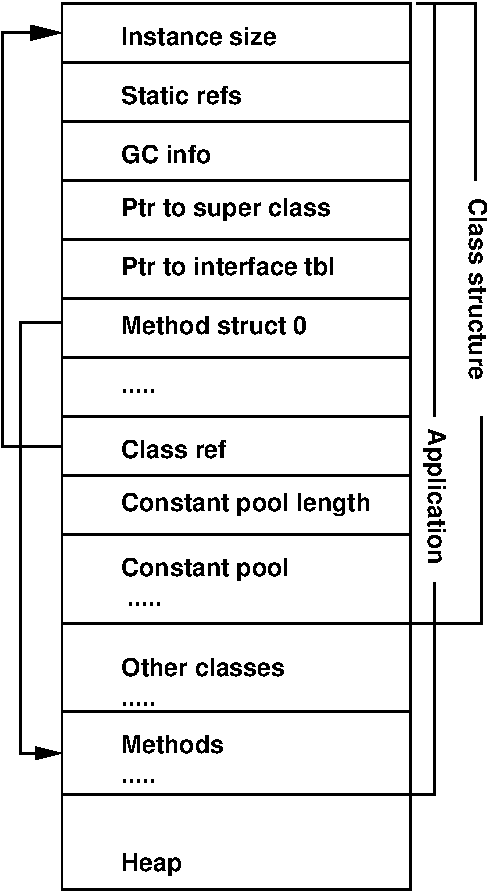
\includegraphics[scale=0.4]{jvmmem}\label{fig:6a}
 }
  \qquad
  \subfloat[Proposed JOP runtime memory organization]{
    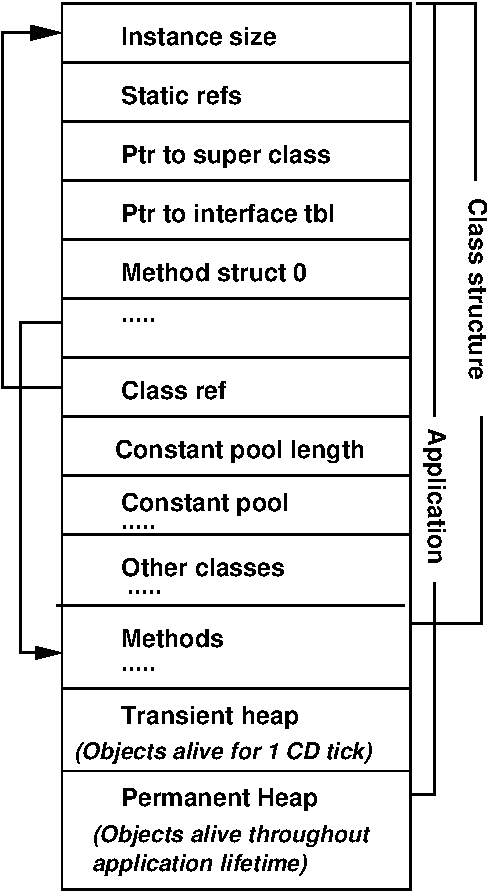
\includegraphics[scale=0.4]{jvmmemn}\label{fig:6b}
  }
  \qquad
  \subfloat[The tool-chain flow]{
    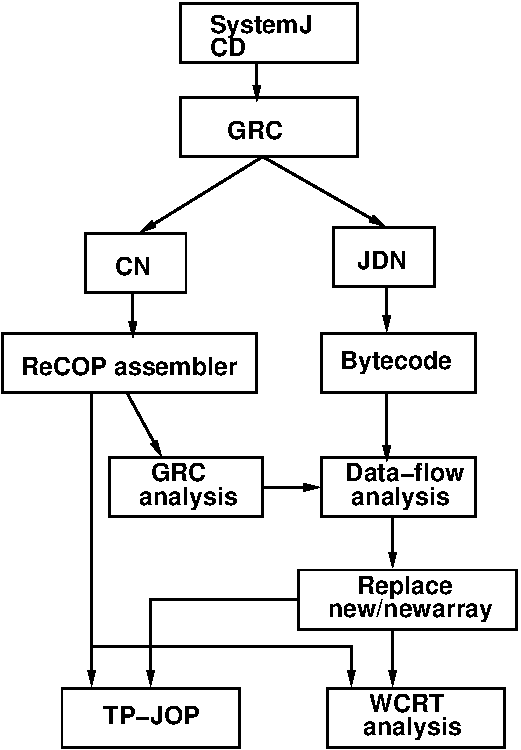
\includegraphics[scale=0.4]{tcflow}
    \label{fig:6c}
  }
  \caption{The tool-chain flow along with the Java runtime memory
    organization in JOP, before and after transformation. The Java stack
    is on separate physical memory as shown in Figure~\ref{fig:3}.}
  \label{fig:6}
\end{figure}

Both runtime memory organizations; original (Figure~\ref{fig:6a}) and
proposed (Figure~\ref{fig:6b}) consists of a number of common elements
required to execute every Java application such as, the constant pool,
method structure table for instance method invocation, references to
static objects, etc. The major point of difference is that the
\textit{GC info} word does not exist in the proposed runtime memory
organization and the \textit{heap} space is divided into two parts; the
transient heap and the permanent heap. Looking at the proposed runtime
memory organization two \underline{requirements} become very important:

\begin{enumerate}
\item There should be no pointer pointing from the permanent heap to the
  transient heap, else an application might terminate at runtime with a
  \texttt{NullPointer} exception -- since the transient heap may be
  reclaimed or overwritten at the end of the clock-domain
  transition. Moreover, in the much worse scenario, an incorrect value
  might be read, in which case the application will be functionally
  incorrect. Both these scenarios are unacceptable for safety-critical
  systems.
\item The permanent heap is never reclaimed and hence, permanent heap
  space should be judiciously allocated. In fact, we need to bound the
  permanent heap space at compile time.
\end{enumerate}

In the rest of the paper we describe compiler transformations that
accomplish the proposed memory management technique.

\section{Static analysis for compile time memory allocation}
\label{sec:comp-analys-stat}

The complete compiler tool-chain flow is shown in
Figure~\ref{fig:6c}. The SystemJ clock-domain is first compiled into the
intermediate GRC format. Next, the control nodes (CN) and the Java data
nodes (JDN) are split and compiled separately into ReCOP native assembly
and Java bytecode, respectively, for execution on the TP-JOP
platform. Two types of compiler analysis are then performed on the
produced native ReCOP assembler and Java bytecode, respectively: (1) GRC
analysis is used to determine the \textit{must} and \textit{may} Java
reachable methods from any given Java program point and (2)
\textit{forward} and \textit{backward} data-flow analysis is performed
to find the objects and arrays that need to be allocated to the
permanent heap. Finally, these object allocation bytecodes need to be
replaced by their time predictable alternatives.

\begin{lrbox}{\eone}
  \begin{minipage}[b]{0.5\linewidth}
    \begin{Verbatim}[numbers=left,commandchars=\\\[\]]
int signal S;\label[l1]
int a = 0;\label[l2]
a = a + 1;\label[l3]
emit S(a);\label[l4]
pause;\label[l7]
/*Variable values can 
 only be carried 
 over tick boundaries
 via signals */
a = #S;\label[l8]
a = a + 1;\label[l5]
emit S(a);\label[l6]
    \end{Verbatim}
  \end{minipage}
\end{lrbox}
\begin{lrbox}{\etwo}
  \begin{minipage}[b]{0.7\linewidth}
    \begin{scriptsize}
      
    \begin{Verbatim}[numbers=left,commandchars=\\\[\]]
public class FruitSorterController {
 //signal S declaration
 private static Signal S;
 private static int a;
 public static void init () {
  S = new Signal();
 }
 public static void main(String args[]){
  init();
  while(true){
   //poll on the method call request from ReCOP
   int methodnum = Native.rd(Const.METHOD_NUM);
   switch(methodnum){\label[e2ss]
    case 0: ...
    ...
    //Call method for 
    //lines \ref[l2] - \ref[l4] (Figure~\ref[fig:7a])
    case 1: Native.wr(RESULT_REG,
    MethodCall1_0());
    //Call method for 
    //lines \ref[l5] - \ref[l6] (Figure \ref[fig:7a])
    case 2: Native.wr(RESULT_REG,
    MethodCall2_0());
   }\label[e2se]
  }
 }
 private static boolean MethodCall1_0(){\label[em1s]
   a = 0;//line \ref[l2], Figure \ref[fig:7a]
   a = a + 1;//line \ref[l3], Figure \ref[fig:7a]
   S.setValue(new Integer(a));
 }\label[em1e]
 private static boolean MethodCall2_0(){\label[em2s]
   a = S.getPreValue(); //get value from previous tick via S
   a = a + 1;
   S.setValue(new Integer(a));
 }\label[em2e]
}
    \end{Verbatim}
    \end{scriptsize}
  \end{minipage}
\end{lrbox}

\begin{figure}[t!]
  \centering
  \subfloat[SystemJ code snippet]{
    \scalebox{0.7}{\usebox{\eone}}
    \label{fig:7a}
  }
  \qquad
  \subfloat[Produced Java code]{
    \scalebox{0.8}{\usebox{\etwo}}
    \label{fig:7b}
  }
  \caption{Example showing the need for GRC and data-flow analysis of a SystemJ program}
  \label{fig:7}
\end{figure}

The need for these two types of analysis can be explained using the
simple example in Figure~\ref{fig:7a}. This SystemJ code snippet
declares a valued signal \texttt{S} (line~\ref{l1}), and an integer
variable \texttt{a} (line~\ref{l2}). Variable \texttt{a} is incremented
(line~\ref{l3}) and emitted via signal \texttt{S} (line~\ref{l4}). After
emission, the tick expires as indicated by the \texttt{pause}
statement. In the second clock-domain transition, variable \texttt{a} is
initialized again, since in SystemJ the only values that are persistent
across ticks are signal values. Variable \texttt{a} is first initialized
to the value held in signal \texttt{S} (from the previous tick) and then
incremented (lines~\ref{l8}-\ref{l5}). The result of this increment is
emitted via signal \texttt{S}. Two methods are produced in the back-end
Java code for execution on JOP (Figure~\ref{fig:7b}). The first method
\texttt{MethodCall1\_0} (lines~\ref{em1s}-\ref{em1e}) initializes
\texttt{a} and then increments it. Finally, it sets the value of the
signal \texttt{S} as the \textit{object} \texttt{a}. The second method
call \texttt{MethodCall2\_0} (lines~\ref{em2s}-\ref{em2e}) increments
the variable \texttt{a} and changes the object reference of signal
\texttt{S}.

Our objective is to find out all the \textit{program-points} that
allocate a new object, whose returned reference is set as a signal value
via the \texttt{setValue} virtual method call on the signal object. We
perform data-flow analysis (ReachDef analysis~\cite{steven1997advanced}
to be exact) to find out such program points in the Java program
generated for execution on JOP (e.g., Figure~\ref{fig:7b}). Fields or
method local object references might be set as signal values and hence,
our data-flow analysis is a context and flow-sensitive intra-procedural
and inter-procedural analysis, i.e., the data-flow analysis not only
examines each Java method, but also traverses the call-graph of the
generated Java program.

A call-graph generated from \textit{just} the Java program is
incomplete, since method calls that \textit{must happen before} a given
program point \textit{appear} as \textit{may happen before} a given
program point. Consider the SystemJ program in Figure~\ref{fig:7a}, we
know for sure that program point at line~\ref{l3} \textit{must} be
executed before program point at line~\ref{l5}. But, in the generated
Java program (Figure~\ref{fig:7b}), the sequential control-flow of the
\textit{SystemJ program} has been turned into branching control-flow
(lines~\ref{e2ss}-\ref{e2se}). Just looking at the Java program, one can
only state with certainty that method \texttt{MethodCall1\_0}
\textit{may} be called before method \texttt{MethodCall2\_0}. More
disconcertingly, just looking at the Java program, one can even say that
method \texttt{MethodCall2\_0} may be called before
\texttt{MethodCall1\_0}, since the dependence edge, which is clear in
the SystemJ program is lost in the generated Java program. The GRC
analysis step produces the may and must method callers for any callee in
the generated Java code. Note that we cannot produce a single Java
method call coalescing the two Java methods: \texttt{MethodCall1\_0} and
\texttt{MethodCall2\_0}, because there is an intertwined control
construct, \texttt{pause}, which needs to be executed on ReCOP. We
describe these GRC and the data-flow analysis steps in the next
sections.

\subsection{AGRC analysis}
\label{sec:agrc-analysis}

%In order to statically determine the worst case memory consumption of a
%program targeting TP-JOP, one needs to analyze codes generated from both
%CNs and JDNs. The compiler is able to trivially determine the maximum
%memory footprint required for executing CN codes from any given SystemJ
%programs [] since there is no dynamic memory allocation required for
%executing this code. On the other hand, the data-flow analysis for JDNs
%is more intricate since it needs to analyze the original AGRC in order
%to retrieve the dependency edges, which are lost after splitting CNs and
%JDNs from the AGRC. We devote this section to illustrate this analysis
%technique.


AGRC is a \textit{directed graph} of tuple $G =(V,E)$, where $V$ is the
set of vertices (nodes of AGRC) and $E$ is the set of ordered pairs of
vertices. Each edge $e = (v_i,v_j), \forall e \in E, v_i \in V, v_j \in
V$ is a tuple denoting that the edge is directed from $v_i$ to $v_j$.
Then a lambda  function $\lambda:v \rightarrow E_i$, $E_i \subseteq E$,
maps \textit{each} vertex to a set of edge(s) where $\forall (v_i,v_j)
\in E_i, v_j = v$ and $E_i$ can be $\emptyset$. When $|E_i| = 1$ we call
$v_i$ \textit{must} be called before $v$ whereas when $|E_i| > 1$ we
call any $v_i \in E_i$ \textit{may} be called before $v$.

\begin{figure}[t!]
	\newsavebox{\codeone}
	\begin{lrbox}{\codeone}
		\begin{minipage}[b]{0.62\textwidth}
		\begin{lstlisting}[tabsize=1,basicstyle=\small\ttfamily,numbers=left]
(mList 
	(mNode JDN1 (Must Null) (May Null))
	(mNode JDN2 
		(Must (mNode JDN1 (Must Null) (May Null))) 
		(May Null))
	(mNode JDN3 
		(Must (mNode JDN1 (Must Null) (May Null))) 
		(May Null))
	(mNode JDN4 (Must Null)
		(May 
			(mNode JDN2 
				(Must (mNode JDN1 (Must Null) (May Null))) 
				(May Null))
			(mNode JDN3 
				(Must (mNode JDN1 (Must Null) (May Null))) 
				(May Null))))
		\end{lstlisting}
	\end{minipage}
	\end{lrbox}

	\centering
	\subfloat[An abstracted AGRC graph]{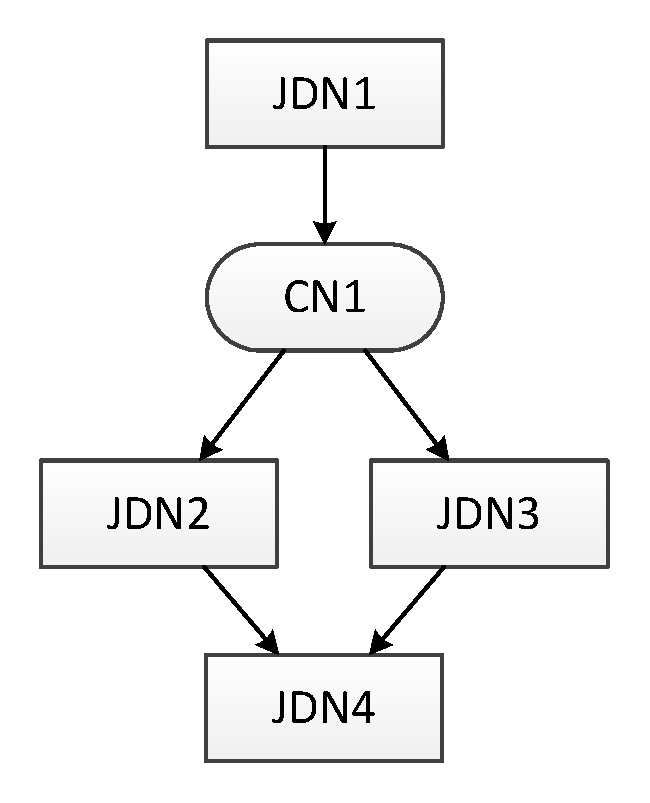
\includegraphics[scale=0.3]{may}
	\label{fig:aagrc}}
	\hspace{1.0cm}
	\subfloat[An output of the AGRC
	analysis]{\scalebox{0.8}{\usebox{\codeone}}\label{fig:tttt}}
	\caption{An example of AGRC analysis}
	\label{fig:maymust}
\end{figure}

In this section, we illustrate how a data-structure, which contains
information on the \textit{may} and \textit{must} relationships between
the nodes, is obtained from the AGRC. Consider a snippet of AGRC graph
shown in Figure~\ref{fig:aagrc}. Here, a root node, \texttt{JDN1}, has
no parent whereas it has an immediate child \texttt{CN1}. \texttt{CN1}
has two children, \texttt{JDN2} and \texttt{JDN3}, and both of these
JDNs have an identical child \texttt{JDN4}. A result of the analysis of
this graph is shown in Figure~\ref{fig:tttt}. An output of the analysis
is a set of nodes called \texttt{mNode}. \texttt{mNode} has three
fields, a node name of type string, \texttt{Must} of type \texttt{mNode}
and \texttt{May} of a set of type \texttt{mNode}. Our analysis tool then
use this data-structure to identify potential callers of each
\texttt{JDN}. For instance, since \texttt{JDN1} has no parents, its
\texttt{Must} and \texttt{May} fields are both \texttt{Null} (line 2).
On the other hand, \texttt{JDN1} must be calling \texttt{JDN2} or
\texttt{JDN3}, hence \texttt{Must} of both \texttt{JDN2} and
\texttt{JDN1} is \texttt{JDN1} (lines 4 and 7). Lastly, \texttt{JDN4}
has two parent nodes; \texttt{JDN2} and \texttt{JDN3}. Therefore, its
\texttt{May} field has both \texttt{JDN2} and \texttt{JDN3} (lines
11-16). It should be noted that we are only interested in callers of
\texttt{JDNs}, hence \texttt{CNs} are not included in the final result
(Figure~\ref{fig:tttt}). A complete algorithm of our AGRC analysis is
shown in Appendix~\ref{ap:1}.






%%% Local Variables:
%%% mode: latex
%%% TeX-master: "jgc"
%%% End:


\subsection{Data-flow analysis}
\label{sec:data-flow-analysis}

\begin{figure}[h!]
  \centering
  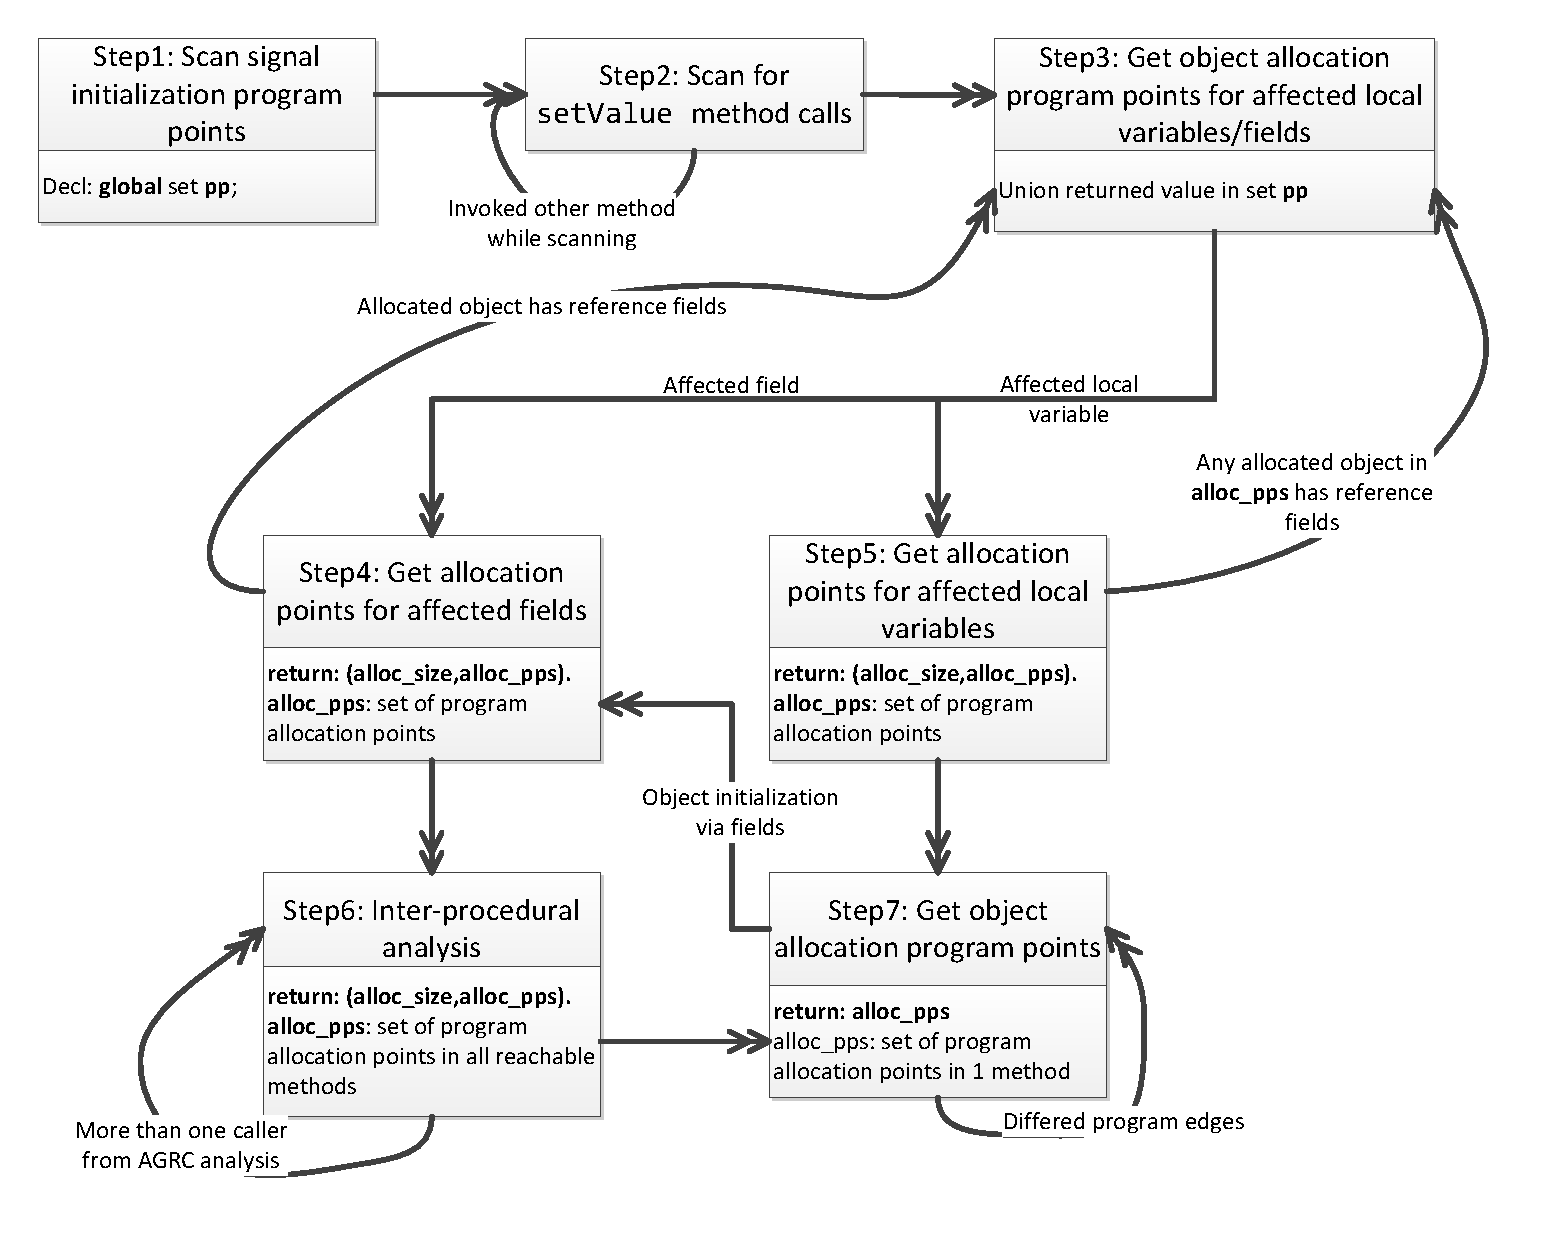
\includegraphics[scale=0.5]{analysis}
  \caption{The flow-chart for the data-flow analysis algorithm}
  \label{fig:fanalysis}
\end{figure}

% As stated previously, we have an intra and inter-procedural
% flow-sensitive data-flow analysis to locate the program points that
% allocate new objects (or arrays) whose returned references are set as
% signal values. Java bytecode is not an ideal format for performing such
% data-flow analysis~\cite{vallee1999soot,hubert2011sawja}, because the
% stack interacts with each bytecode operation, which means that data-flow
% analysis would need simulating the stack state. In order to avoid
% simulating the stack itself, we (like other Java static analysis
% frameworks~\cite{vallee1999soot,hubert2011sawja}) first convert the
% bytecode into a register-transfer level (RTL) intermediate format. For
% this work, we have used the OCaml~\cite{leroy1998ocaml} based Java
% static analysis framework; Sawja's~\cite{hubert2011sawja} intermediate
% RTL format called \textit{Bytecode Intermediate Representation} (BIR).

\newsavebox{\exonec}
\begin{lrbox}{\exonec}
  \begin{minipage}[b]{0.7\linewidth}
    \begin{Verbatim}[numbers=left,commandchars=\\\[\]]
public static void main (String args) {
 init ();
 MethodCall0_4();
}
    \end{Verbatim}
  \end{minipage}
\end{lrbox}

\newsavebox{\exone}
\begin{lrbox}{\exone}
  \begin{minipage}[b]{0.7\linewidth}
    \begin{Verbatim}[numbers=left,commandchars=\\\[\]]
private static Signal S;\label[exone:sdec]
private static boolean a_thread_2;
public static void init () {
 S = new Signal();\label[exone:siginit]
}
public boolean MethodCall0_4() {
 b B = new b(33);
 c C = new c(1001,101);
 a t;\label[exone:tdec]
 /* Use polymorphism for equality */
 a_thread_2 = true;
 if (a_thread_2){
  int b1 = B.getb1();
  t = new b(b1);/*Making deep copies*/\label[exone:l1]
  ((b)t).bbb = new Integer(99);
 }
 else {
  int cc = C.getcc();
  int ccc = C.getccc();
  t = new c(cc,ccc);/*Making deep copies*/\label[exone:l2]
  ((c)t).mm = new Integer(999);\label[exone:l33]
 }
 /* Emit t via S */
 S.setValue(t);\label[exone:s2l1]
 if (a_thread_2)\label[exone:l3]
  /* Print */
  System.out.println(((b)S.getValue()).bb);
 else {
  /* Print */
  System.out.println(((c)S.getValue()).cc);
  System.out.println(((c)S.getValue()).ccc);
 }\label[exone:l4]
 return true;  
}
    \end{Verbatim}
  \end{minipage}
\end{lrbox}

\newsavebox{\extwo}
\begin{lrbox}{\extwo}
  \begin{minipage}[b]{0.7\linewidth}
    \begin{Verbatim}[numbers=left,commandchars=\\\[\]]
private static Signal S;
private static a A;
public static void main(String args[]){
 A = new a();\label[extwo:l2]
 A.b = new Integer (70);\label[extwo:l3]
 MethodCall0_0();
}
public boolean MethodCall0_0(){
 /* Test 1 */
 S.setValue(A);\label[extwo:l1]
 return false;
}
    \end{Verbatim}
  \end{minipage}
\end{lrbox}

\begin{figure}[t!]
  % \centering
  \subfloat[The call-graph for the running example]{
    \scalebox{0.5}{% Graphic for TeX using PGF
% Title: I:\Avinash\jpaper\Callgraph.dia
% Creator: Dia v0.97.2
% CreationDate: Tue May 26 14:50:53 2015
% For: amal029
% \usepackage{tikz}
% The following commands are not supported in PSTricks at present
% We define them conditionally, so when they are implemented,
% this pgf file will use them.
\ifx\du\undefined
  \newlength{\du}
\fi
\setlength{\du}{15\unitlength}
\begin{tikzpicture}
\pgftransformxscale{1.000000}
\pgftransformyscale{-1.000000}
\definecolor{dialinecolor}{rgb}{0.000000, 0.000000, 0.000000}
\pgfsetstrokecolor{dialinecolor}
\definecolor{dialinecolor}{rgb}{1.000000, 1.000000, 1.000000}
\pgfsetfillcolor{dialinecolor}
\definecolor{dialinecolor}{rgb}{1.000000, 1.000000, 1.000000}
\pgfsetfillcolor{dialinecolor}
\fill (23.000000\du,9.285690\du)--(23.000000\du,12.000001\du)--(29.900000\du,12.000001\du)--(29.900000\du,9.285690\du)--cycle;
\pgfsetlinewidth{0.100000\du}
\pgfsetdash{}{0pt}
\pgfsetdash{}{0pt}
\pgfsetmiterjoin
\definecolor{dialinecolor}{rgb}{0.000000, 0.000000, 0.000000}
\pgfsetstrokecolor{dialinecolor}
\draw (23.000000\du,9.285690\du)--(23.000000\du,12.000001\du)--(29.900000\du,12.000001\du)--(29.900000\du,9.285690\du)--cycle;
% setfont left to latex
\definecolor{dialinecolor}{rgb}{0.000000, 0.000000, 0.000000}
\pgfsetstrokecolor{dialinecolor}
\node[anchor=west] at (23.450000\du,10.433190\du){1:init();};
% setfont left to latex
\definecolor{dialinecolor}{rgb}{0.000000, 0.000000, 0.000000}
\pgfsetstrokecolor{dialinecolor}
\node[anchor=west] at (23.450000\du,11.240346\du){2:MCall();};
\definecolor{dialinecolor}{rgb}{1.000000, 1.000000, 1.000000}
\pgfsetfillcolor{dialinecolor}
\fill (27.045000\du,15.134300\du)--(27.045000\du,17.848611\du)--(34.732500\du,17.848611\du)--(34.732500\du,15.134300\du)--cycle;
\pgfsetlinewidth{0.100000\du}
\pgfsetdash{}{0pt}
\pgfsetdash{}{0pt}
\pgfsetmiterjoin
\definecolor{dialinecolor}{rgb}{0.000000, 0.000000, 0.000000}
\pgfsetstrokecolor{dialinecolor}
\draw (27.045000\du,15.134300\du)--(27.045000\du,17.848611\du)--(34.732500\du,17.848611\du)--(34.732500\du,15.134300\du)--cycle;
% setfont left to latex
\definecolor{dialinecolor}{rgb}{0.000000, 0.000000, 0.000000}
\pgfsetstrokecolor{dialinecolor}
\node[anchor=west] at (27.495000\du,16.685378\du){.....///code};
\pgfsetlinewidth{0.100000\du}
\pgfsetdash{}{0pt}
\pgfsetdash{}{0pt}
\pgfsetmiterjoin
\pgfsetbuttcap
{
\definecolor{dialinecolor}{rgb}{0.000000, 0.000000, 0.000000}
\pgfsetfillcolor{dialinecolor}
% was here!!!
\pgfsetarrowsend{stealth}
{\pgfsetcornersarced{\pgfpoint{0.000000\du}{0.000000\du}}\definecolor{dialinecolor}{rgb}{0.000000, 0.000000, 0.000000}
\pgfsetstrokecolor{dialinecolor}
\draw (26.450000\du,12.000001\du)--(26.450000\du,13.575001\du)--(21.200000\du,13.575001\du)--(21.200000\du,15.150000\du);
}}
\pgfsetlinewidth{0.100000\du}
\pgfsetdash{}{0pt}
\pgfsetdash{}{0pt}
\pgfsetmiterjoin
\pgfsetbuttcap
{
\definecolor{dialinecolor}{rgb}{0.000000, 0.000000, 0.000000}
\pgfsetfillcolor{dialinecolor}
% was here!!!
\pgfsetarrowsend{stealth}
{\pgfsetcornersarced{\pgfpoint{0.000000\du}{0.000000\du}}\definecolor{dialinecolor}{rgb}{0.000000, 0.000000, 0.000000}
\pgfsetstrokecolor{dialinecolor}
\draw (26.450000\du,12.000000\du)--(26.450000\du,13.600000\du)--(30.888800\du,13.600000\du)--(30.888800\du,15.134300\du);
}}
% setfont left to latex
\definecolor{dialinecolor}{rgb}{0.000000, 0.000000, 0.000000}
\pgfsetstrokecolor{dialinecolor}
\node[anchor=west] at (23.207600\du,8.994270\du){main method};
% setfont left to latex
\definecolor{dialinecolor}{rgb}{0.000000, 0.000000, 0.000000}
\pgfsetstrokecolor{dialinecolor}
\node[anchor=west] at (18.707600\du,19.244300\du){init method};
% setfont left to latex
\definecolor{dialinecolor}{rgb}{0.000000, 0.000000, 0.000000}
\pgfsetstrokecolor{dialinecolor}
\node[anchor=west] at (28.352600\du,18.764300\du){MCall method};
\definecolor{dialinecolor}{rgb}{1.000000, 1.000000, 1.000000}
\pgfsetfillcolor{dialinecolor}
\fill (16.300000\du,15.150000\du)--(16.300000\du,18.400000\du)--(26.100000\du,18.400000\du)--(26.100000\du,15.150000\du)--cycle;
\pgfsetlinewidth{0.100000\du}
\pgfsetdash{}{0pt}
\pgfsetdash{}{0pt}
\pgfsetmiterjoin
\definecolor{dialinecolor}{rgb}{0.000000, 0.000000, 0.000000}
\pgfsetstrokecolor{dialinecolor}
\draw (16.300000\du,15.150000\du)--(16.300000\du,18.400000\du)--(26.100000\du,18.400000\du)--(26.100000\du,15.150000\du)--cycle;
% setfont left to latex
\definecolor{dialinecolor}{rgb}{0.000000, 0.000000, 0.000000}
\pgfsetstrokecolor{dialinecolor}
\node[anchor=west] at (16.750000\du,16.968922\du){};
\definecolor{dialinecolor}{rgb}{1.000000, 1.000000, 1.000000}
\pgfsetfillcolor{dialinecolor}
\fill (16.920000\du,15.441456\du)--(16.920000\du,17.348611\du)--(25.382500\du,17.348611\du)--(25.382500\du,15.441456\du)--cycle;
\pgfsetlinewidth{0.100000\du}
\pgfsetdash{}{0pt}
\pgfsetdash{}{0pt}
\pgfsetmiterjoin
\definecolor{dialinecolor}{rgb}{0.000000, 0.000000, 0.000000}
\pgfsetstrokecolor{dialinecolor}
\draw (16.920000\du,15.441456\du)--(16.920000\du,17.348611\du)--(25.382500\du,17.348611\du)--(25.382500\du,15.441456\du)--cycle;
% setfont left to latex
\definecolor{dialinecolor}{rgb}{0.000000, 0.000000, 0.000000}
\pgfsetstrokecolor{dialinecolor}
\node[anchor=west] at (17.370000\du,16.588956\du){1:S = new Signal();};
% setfont left to latex
\definecolor{dialinecolor}{rgb}{0.000000, 0.000000, 0.000000}
\pgfsetstrokecolor{dialinecolor}
\node[anchor=west] at (17.050000\du,18.075000\du){BB1};
\end{tikzpicture}
}
    % \scalebox{0.7}{\usebox{\exonec}}
    \label{fig:8hc}
  }
  \qquad
  \subfloat[The control-flow graph of the MCall method]{
    \scalebox{0.5}{% Graphic for TeX using PGF
% Title: D:\jpaper\MCall.dia
% Creator: Dia v0.97.2
% CreationDate: Wed May 13 14:47:23 2015
% For: amal029
% \usepackage{tikz}
% The following commands are not supported in PSTricks at present
% We define them conditionally, so when they are implemented,
% this pgf file will use them.
\ifx\du\undefined
  \newlength{\du}
\fi
\setlength{\du}{15\unitlength}
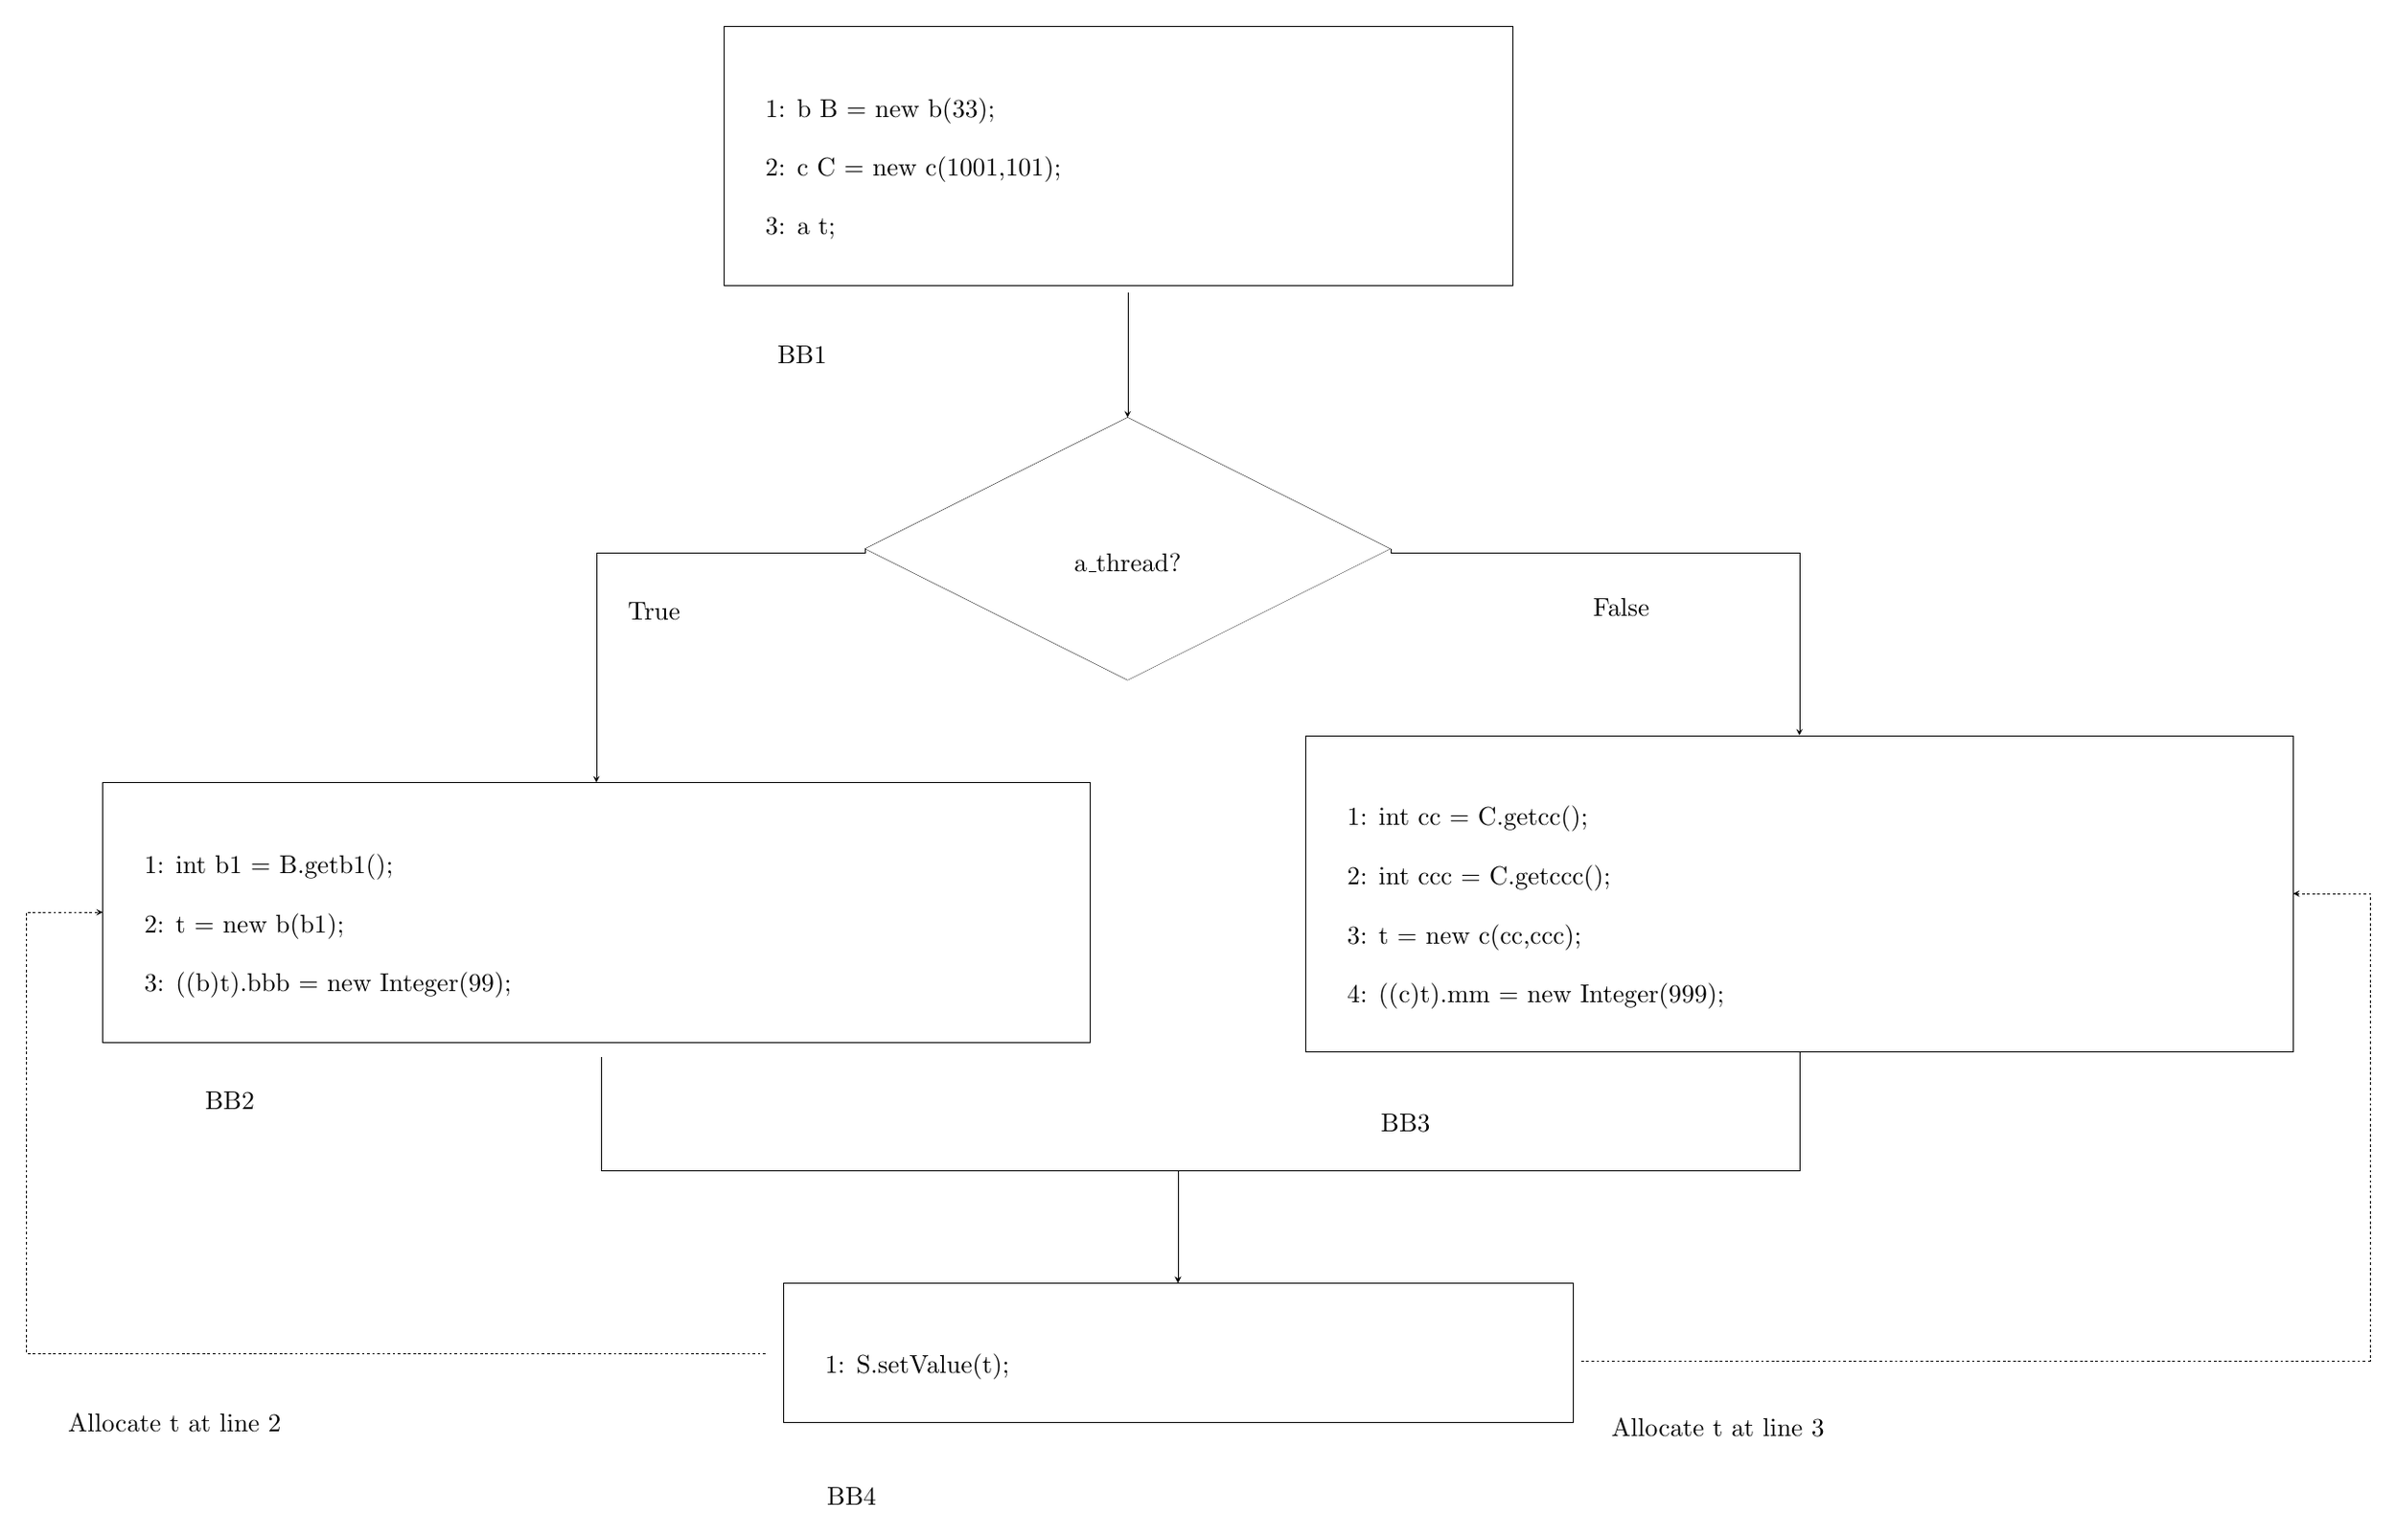
\begin{tikzpicture}
\pgftransformxscale{1.000000}
\pgftransformyscale{-1.000000}
\definecolor{dialinecolor}{rgb}{0.000000, 0.000000, 0.000000}
\pgfsetstrokecolor{dialinecolor}
\definecolor{dialinecolor}{rgb}{1.000000, 1.000000, 1.000000}
\pgfsetfillcolor{dialinecolor}
\definecolor{dialinecolor}{rgb}{1.000000, 1.000000, 1.000000}
\pgfsetfillcolor{dialinecolor}
\fill (22.981250\du,7.850000\du)--(22.981250\du,11.400000\du)--(33.768750\du,11.400000\du)--(33.768750\du,7.850000\du)--cycle;
\pgfsetlinewidth{0.100000\du}
\pgfsetdash{}{0pt}
\pgfsetdash{}{0pt}
\pgfsetmiterjoin
\definecolor{dialinecolor}{rgb}{0.000000, 0.000000, 0.000000}
\pgfsetstrokecolor{dialinecolor}
\draw (22.981250\du,7.850000\du)--(22.981250\du,11.400000\du)--(33.768750\du,11.400000\du)--(33.768750\du,7.850000\du)--cycle;
% setfont left to latex
\definecolor{dialinecolor}{rgb}{0.000000, 0.000000, 0.000000}
\pgfsetstrokecolor{dialinecolor}
\node[anchor=west] at (23.431250\du,9.011767\du){1: b B = new b(33);};
% setfont left to latex
\definecolor{dialinecolor}{rgb}{0.000000, 0.000000, 0.000000}
\pgfsetstrokecolor{dialinecolor}
\node[anchor=west] at (23.431250\du,9.818922\du){2: c C = new c(1001,101);};
% setfont left to latex
\definecolor{dialinecolor}{rgb}{0.000000, 0.000000, 0.000000}
\pgfsetstrokecolor{dialinecolor}
\node[anchor=west] at (23.431250\du,10.626078\du){3: a t;};
% setfont left to latex
\definecolor{dialinecolor}{rgb}{0.000000, 0.000000, 0.000000}
\pgfsetstrokecolor{dialinecolor}
\node at (24.050000\du,12.350000\du){BB1};
\definecolor{dialinecolor}{rgb}{1.000000, 1.000000, 1.000000}
\pgfsetfillcolor{dialinecolor}
\fill (28.500000\du,13.203420\du)--(32.093160\du,15.000000\du)--(28.500000\du,16.796580\du)--(24.906840\du,15.000000\du)--cycle;
\pgfsetlinewidth{0.100000\du}
\pgfsetdash{}{0pt}
\pgfsetdash{}{0pt}
\pgfsetmiterjoin
\definecolor{dialinecolor}{rgb}{0.000000, 0.000000, 0.000000}
\pgfsetstrokecolor{dialinecolor}
\draw (28.500000\du,13.203420\du)--(32.093160\du,15.000000\du)--(28.500000\du,16.796580\du)--(24.906840\du,15.000000\du)--cycle;
% setfont left to latex
\definecolor{dialinecolor}{rgb}{0.000000, 0.000000, 0.000000}
\pgfsetstrokecolor{dialinecolor}
\node at (28.500000\du,15.195000\du){a\_thread?};
\pgfsetlinewidth{0.100000\du}
\pgfsetdash{}{0pt}
\pgfsetdash{}{0pt}
\pgfsetbuttcap
{
\definecolor{dialinecolor}{rgb}{0.000000, 0.000000, 0.000000}
\pgfsetfillcolor{dialinecolor}
% was here!!!
\pgfsetarrowsend{stealth}
\definecolor{dialinecolor}{rgb}{0.000000, 0.000000, 0.000000}
\pgfsetstrokecolor{dialinecolor}
\draw (28.500000\du,11.500000\du)--(28.500000\du,13.203420\du);
}
\definecolor{dialinecolor}{rgb}{1.000000, 1.000000, 1.000000}
\pgfsetfillcolor{dialinecolor}
\fill (14.488750\du,18.195000\du)--(14.488750\du,21.745000\du)--(27.988750\du,21.745000\du)--(27.988750\du,18.195000\du)--cycle;
\pgfsetlinewidth{0.100000\du}
\pgfsetdash{}{0pt}
\pgfsetdash{}{0pt}
\pgfsetmiterjoin
\definecolor{dialinecolor}{rgb}{0.000000, 0.000000, 0.000000}
\pgfsetstrokecolor{dialinecolor}
\draw (14.488750\du,18.195000\du)--(14.488750\du,21.745000\du)--(27.988750\du,21.745000\du)--(27.988750\du,18.195000\du)--cycle;
% setfont left to latex
\definecolor{dialinecolor}{rgb}{0.000000, 0.000000, 0.000000}
\pgfsetstrokecolor{dialinecolor}
\node[anchor=west] at (14.938750\du,19.356767\du){1: int b1 = B.getb1();};
% setfont left to latex
\definecolor{dialinecolor}{rgb}{0.000000, 0.000000, 0.000000}
\pgfsetstrokecolor{dialinecolor}
\node[anchor=west] at (14.938750\du,20.163922\du){2: t = new b(b1);};
% setfont left to latex
\definecolor{dialinecolor}{rgb}{0.000000, 0.000000, 0.000000}
\pgfsetstrokecolor{dialinecolor}
\node[anchor=west] at (14.938750\du,20.971078\du){3: ((b)t).bbb = new Integer(99);};
\definecolor{dialinecolor}{rgb}{1.000000, 1.000000, 1.000000}
\pgfsetfillcolor{dialinecolor}
\fill (30.933750\du,17.550689\du)--(30.933750\du,21.879311\du)--(44.433750\du,21.879311\du)--(44.433750\du,17.550689\du)--cycle;
\pgfsetlinewidth{0.100000\du}
\pgfsetdash{}{0pt}
\pgfsetdash{}{0pt}
\pgfsetmiterjoin
\definecolor{dialinecolor}{rgb}{0.000000, 0.000000, 0.000000}
\pgfsetstrokecolor{dialinecolor}
\draw (30.933750\du,17.550689\du)--(30.933750\du,21.879311\du)--(44.433750\du,21.879311\du)--(44.433750\du,17.550689\du)--cycle;
% setfont left to latex
\definecolor{dialinecolor}{rgb}{0.000000, 0.000000, 0.000000}
\pgfsetstrokecolor{dialinecolor}
\node[anchor=west] at (31.383750\du,18.698189\du){1: int cc = C.getcc();};
% setfont left to latex
\definecolor{dialinecolor}{rgb}{0.000000, 0.000000, 0.000000}
\pgfsetstrokecolor{dialinecolor}
\node[anchor=west] at (31.383750\du,19.505344\du){2: int ccc = C.getccc();};
% setfont left to latex
\definecolor{dialinecolor}{rgb}{0.000000, 0.000000, 0.000000}
\pgfsetstrokecolor{dialinecolor}
\node[anchor=west] at (31.383750\du,20.312500\du){3: t = new c(cc,ccc);};
% setfont left to latex
\definecolor{dialinecolor}{rgb}{0.000000, 0.000000, 0.000000}
\pgfsetstrokecolor{dialinecolor}
\node[anchor=west] at (31.383750\du,21.119656\du){4: ((c)t).mm = new Integer(999);};
% setfont left to latex
\definecolor{dialinecolor}{rgb}{0.000000, 0.000000, 0.000000}
\pgfsetstrokecolor{dialinecolor}
\node at (16.227500\du,22.552500\du){BB2};
% setfont left to latex
\definecolor{dialinecolor}{rgb}{0.000000, 0.000000, 0.000000}
\pgfsetstrokecolor{dialinecolor}
\node at (32.300000\du,22.850000\du){BB3};
\pgfsetlinewidth{0.100000\du}
\pgfsetdash{}{0pt}
\pgfsetdash{}{0pt}
\pgfsetmiterjoin
\pgfsetbuttcap
{
\definecolor{dialinecolor}{rgb}{0.000000, 0.000000, 0.000000}
\pgfsetfillcolor{dialinecolor}
% was here!!!
\pgfsetarrowsend{stealth}
{\pgfsetcornersarced{\pgfpoint{0.000000\du}{0.000000\du}}\definecolor{dialinecolor}{rgb}{0.000000, 0.000000, 0.000000}
\pgfsetstrokecolor{dialinecolor}
\draw (24.906840\du,15.000000\du)--(24.906840\du,15.050000\du)--(21.238750\du,15.050000\du)--(21.238750\du,18.195000\du);
}}
\pgfsetlinewidth{0.100000\du}
\pgfsetdash{}{0pt}
\pgfsetdash{}{0pt}
\pgfsetmiterjoin
\pgfsetbuttcap
{
\definecolor{dialinecolor}{rgb}{0.000000, 0.000000, 0.000000}
\pgfsetfillcolor{dialinecolor}
% was here!!!
\pgfsetarrowsend{stealth}
{\pgfsetcornersarced{\pgfpoint{0.000000\du}{0.000000\du}}\definecolor{dialinecolor}{rgb}{0.000000, 0.000000, 0.000000}
\pgfsetstrokecolor{dialinecolor}
\draw (32.093160\du,15.000000\du)--(32.093160\du,15.050000\du)--(37.683750\du,15.050000\du)--(37.683750\du,17.550689\du);
}}
% setfont left to latex
\definecolor{dialinecolor}{rgb}{0.000000, 0.000000, 0.000000}
\pgfsetstrokecolor{dialinecolor}
\node[anchor=west] at (21.550000\du,15.850000\du){True};
% setfont left to latex
\definecolor{dialinecolor}{rgb}{0.000000, 0.000000, 0.000000}
\pgfsetstrokecolor{dialinecolor}
\node[anchor=west] at (34.745000\du,15.802500\du){False};
\definecolor{dialinecolor}{rgb}{1.000000, 1.000000, 1.000000}
\pgfsetfillcolor{dialinecolor}
\fill (23.795000\du,25.037844\du)--(23.795000\du,26.945000\du)--(34.582500\du,26.945000\du)--(34.582500\du,25.037844\du)--cycle;
\pgfsetlinewidth{0.100000\du}
\pgfsetdash{}{0pt}
\pgfsetdash{}{0pt}
\pgfsetmiterjoin
\definecolor{dialinecolor}{rgb}{0.000000, 0.000000, 0.000000}
\pgfsetstrokecolor{dialinecolor}
\draw (23.795000\du,25.037844\du)--(23.795000\du,26.945000\du)--(34.582500\du,26.945000\du)--(34.582500\du,25.037844\du)--cycle;
% setfont left to latex
\definecolor{dialinecolor}{rgb}{0.000000, 0.000000, 0.000000}
\pgfsetstrokecolor{dialinecolor}
\node[anchor=west] at (24.245000\du,26.185344\du){1: S.setValue(t);};
% setfont left to latex
\definecolor{dialinecolor}{rgb}{0.000000, 0.000000, 0.000000}
\pgfsetstrokecolor{dialinecolor}
\node at (24.727500\du,27.952500\du){BB4};
\pgfsetlinewidth{0.100000\du}
\pgfsetdash{}{0pt}
\pgfsetdash{}{0pt}
\pgfsetmiterjoin
\pgfsetbuttcap
{
\definecolor{dialinecolor}{rgb}{0.000000, 0.000000, 0.000000}
\pgfsetfillcolor{dialinecolor}
% was here!!!
\pgfsetarrowsend{stealth}
{\pgfsetcornersarced{\pgfpoint{0.000000\du}{0.000000\du}}\definecolor{dialinecolor}{rgb}{0.000000, 0.000000, 0.000000}
\pgfsetstrokecolor{dialinecolor}
\draw (21.300000\du,21.950000\du)--(21.300000\du,23.493922\du)--(29.188750\du,23.493922\du)--(29.188750\du,25.037844\du);
}}
\pgfsetlinewidth{0.100000\du}
\pgfsetdash{}{0pt}
\pgfsetdash{}{0pt}
\pgfsetmiterjoin
\pgfsetbuttcap
{
\definecolor{dialinecolor}{rgb}{0.000000, 0.000000, 0.000000}
\pgfsetfillcolor{dialinecolor}
% was here!!!
\pgfsetarrowsend{stealth}
{\pgfsetcornersarced{\pgfpoint{0.000000\du}{0.000000\du}}\definecolor{dialinecolor}{rgb}{0.000000, 0.000000, 0.000000}
\pgfsetstrokecolor{dialinecolor}
\draw (37.683750\du,21.879311\du)--(37.683750\du,23.500000\du)--(29.188750\du,23.500000\du)--(29.188750\du,25.037844\du);
}}
\pgfsetlinewidth{0.100000\du}
\pgfsetdash{{1.000000\du}{1.000000\du}}{0\du}
\pgfsetdash{{1.000000\du}{1.000000\du}}{0\du}
\pgfsetmiterjoin
\pgfsetbuttcap
{
\definecolor{dialinecolor}{rgb}{0.000000, 0.000000, 0.000000}
\pgfsetfillcolor{dialinecolor}
% was here!!!
\pgfsetarrowsend{stealth}
{\pgfsetcornersarced{\pgfpoint{0.000000\du}{0.000000\du}}\definecolor{dialinecolor}{rgb}{0.000000, 0.000000, 0.000000}
\pgfsetstrokecolor{dialinecolor}
\draw (23.550000\du,26.000000\du)--(13.438750\du,26.000000\du)--(13.438750\du,19.970000\du)--(14.488750\du,19.970000\du);
}}
% setfont left to latex
\definecolor{dialinecolor}{rgb}{0.000000, 0.000000, 0.000000}
\pgfsetstrokecolor{dialinecolor}
\node[anchor=west] at (13.900000\du,26.950000\du){Allocate t at line 2};
\pgfsetlinewidth{0.100000\du}
\pgfsetdash{{1.000000\du}{1.000000\du}}{0\du}
\pgfsetdash{{1.000000\du}{1.000000\du}}{0\du}
\pgfsetmiterjoin
\pgfsetbuttcap
{
\definecolor{dialinecolor}{rgb}{0.000000, 0.000000, 0.000000}
\pgfsetfillcolor{dialinecolor}
% was here!!!
\pgfsetarrowsend{stealth}
{\pgfsetcornersarced{\pgfpoint{0.000000\du}{0.000000\du}}\definecolor{dialinecolor}{rgb}{0.000000, 0.000000, 0.000000}
\pgfsetstrokecolor{dialinecolor}
\draw (34.700000\du,26.100000\du)--(45.483750\du,26.100000\du)--(45.483750\du,19.715000\du)--(44.433750\du,19.715000\du);
}}
% setfont left to latex
\definecolor{dialinecolor}{rgb}{0.000000, 0.000000, 0.000000}
\pgfsetstrokecolor{dialinecolor}
\node[anchor=west] at (34.995000\du,27.020000\du){Allocate t at line 3};
\end{tikzpicture}
}
    % \scalebox{0.7}{\usebox{\exone}}
    \label{fig:8h}
  }
  \caption{Running example used to explain the intra-procedural
    data-flow analysis}
  \label{fig:8}
\end{figure}

\begin{figure}[t!]
  \centering
  \subfloat[UML class hierarchy for classes \texttt{a}, \texttt{b} and
  \texttt{c} used in Figure~\ref{fig:8h}]{
    \scalebox{0.5}{% Graphic for TeX using PGF
% Title: D:\jpaper\UML.dia
% Creator: Dia v0.97.2
% CreationDate: Wed May 13 11:28:56 2015
% For: amal029
% \usepackage{tikz}
% The following commands are not supported in PSTricks at present
% We define them conditionally, so when they are implemented,
% this pgf file will use them.
\ifx\du\undefined
  \newlength{\du}
\fi
\setlength{\du}{15\unitlength}
\begin{tikzpicture}
\pgftransformxscale{1.000000}
\pgftransformyscale{-1.000000}
\definecolor{dialinecolor}{rgb}{0.000000, 0.000000, 0.000000}
\pgfsetstrokecolor{dialinecolor}
\definecolor{dialinecolor}{rgb}{1.000000, 1.000000, 1.000000}
\pgfsetfillcolor{dialinecolor}
\pgfsetlinewidth{0.100000\du}
\pgfsetdash{}{0pt}
\definecolor{dialinecolor}{rgb}{1.000000, 1.000000, 1.000000}
\pgfsetfillcolor{dialinecolor}
\fill (20.500000\du,13.050000\du)--(20.500000\du,14.450000\du)--(26.005000\du,14.450000\du)--(26.005000\du,13.050000\du)--cycle;
\definecolor{dialinecolor}{rgb}{0.000000, 0.000000, 0.000000}
\pgfsetstrokecolor{dialinecolor}
\draw (20.500000\du,13.050000\du)--(20.500000\du,14.450000\du)--(26.005000\du,14.450000\du)--(26.005000\du,13.050000\du)--cycle;
% setfont left to latex
\definecolor{dialinecolor}{rgb}{0.000000, 0.000000, 0.000000}
\pgfsetstrokecolor{dialinecolor}
\node at (23.252500\du,14.000000\du){Class b};
\definecolor{dialinecolor}{rgb}{1.000000, 1.000000, 1.000000}
\pgfsetfillcolor{dialinecolor}
\fill (20.500000\du,14.450000\du)--(20.500000\du,16.250000\du)--(26.005000\du,16.250000\du)--(26.005000\du,14.450000\du)--cycle;
\definecolor{dialinecolor}{rgb}{0.000000, 0.000000, 0.000000}
\pgfsetstrokecolor{dialinecolor}
\draw (20.500000\du,14.450000\du)--(20.500000\du,16.250000\du)--(26.005000\du,16.250000\du)--(26.005000\du,14.450000\du)--cycle;
% setfont left to latex
\definecolor{dialinecolor}{rgb}{0.000000, 0.000000, 0.000000}
\pgfsetstrokecolor{dialinecolor}
\node[anchor=west] at (20.650000\du,15.150000\du){+bf1: int};
% setfont left to latex
\definecolor{dialinecolor}{rgb}{0.000000, 0.000000, 0.000000}
\pgfsetstrokecolor{dialinecolor}
\node[anchor=west] at (20.650000\du,15.950000\du){+bf2: Integer};
\definecolor{dialinecolor}{rgb}{1.000000, 1.000000, 1.000000}
\pgfsetfillcolor{dialinecolor}
\fill (20.500000\du,16.250000\du)--(20.500000\du,16.650000\du)--(26.005000\du,16.650000\du)--(26.005000\du,16.250000\du)--cycle;
\definecolor{dialinecolor}{rgb}{0.000000, 0.000000, 0.000000}
\pgfsetstrokecolor{dialinecolor}
\draw (20.500000\du,16.250000\du)--(20.500000\du,16.650000\du)--(26.005000\du,16.650000\du)--(26.005000\du,16.250000\du)--cycle;
\pgfsetlinewidth{0.100000\du}
\pgfsetdash{}{0pt}
\definecolor{dialinecolor}{rgb}{1.000000, 1.000000, 1.000000}
\pgfsetfillcolor{dialinecolor}
\fill (25.950000\du,8.050000\du)--(25.950000\du,9.450000\du)--(30.685000\du,9.450000\du)--(30.685000\du,8.050000\du)--cycle;
\definecolor{dialinecolor}{rgb}{0.000000, 0.000000, 0.000000}
\pgfsetstrokecolor{dialinecolor}
\draw (25.950000\du,8.050000\du)--(25.950000\du,9.450000\du)--(30.685000\du,9.450000\du)--(30.685000\du,8.050000\du)--cycle;
% setfont left to latex
\definecolor{dialinecolor}{rgb}{0.000000, 0.000000, 0.000000}
\pgfsetstrokecolor{dialinecolor}
\node at (28.317500\du,9.000000\du){Class a};
\definecolor{dialinecolor}{rgb}{1.000000, 1.000000, 1.000000}
\pgfsetfillcolor{dialinecolor}
\fill (25.950000\du,9.450000\du)--(25.950000\du,10.450000\du)--(30.685000\du,10.450000\du)--(30.685000\du,9.450000\du)--cycle;
\definecolor{dialinecolor}{rgb}{0.000000, 0.000000, 0.000000}
\pgfsetstrokecolor{dialinecolor}
\draw (25.950000\du,9.450000\du)--(25.950000\du,10.450000\du)--(30.685000\du,10.450000\du)--(30.685000\du,9.450000\du)--cycle;
% setfont left to latex
\definecolor{dialinecolor}{rgb}{0.000000, 0.000000, 0.000000}
\pgfsetstrokecolor{dialinecolor}
\node[anchor=west] at (26.100000\du,10.150000\du){+af1: Integer};
\definecolor{dialinecolor}{rgb}{1.000000, 1.000000, 1.000000}
\pgfsetfillcolor{dialinecolor}
\fill (25.950000\du,10.450000\du)--(25.950000\du,10.850000\du)--(30.685000\du,10.850000\du)--(30.685000\du,10.450000\du)--cycle;
\definecolor{dialinecolor}{rgb}{0.000000, 0.000000, 0.000000}
\pgfsetstrokecolor{dialinecolor}
\draw (25.950000\du,10.450000\du)--(25.950000\du,10.850000\du)--(30.685000\du,10.850000\du)--(30.685000\du,10.450000\du)--cycle;
\pgfsetlinewidth{0.100000\du}
\pgfsetdash{}{0pt}
\definecolor{dialinecolor}{rgb}{1.000000, 1.000000, 1.000000}
\pgfsetfillcolor{dialinecolor}
\fill (30.700000\du,13.050000\du)--(30.700000\du,14.450000\du)--(35.820000\du,14.450000\du)--(35.820000\du,13.050000\du)--cycle;
\definecolor{dialinecolor}{rgb}{0.000000, 0.000000, 0.000000}
\pgfsetstrokecolor{dialinecolor}
\draw (30.700000\du,13.050000\du)--(30.700000\du,14.450000\du)--(35.820000\du,14.450000\du)--(35.820000\du,13.050000\du)--cycle;
% setfont left to latex
\definecolor{dialinecolor}{rgb}{0.000000, 0.000000, 0.000000}
\pgfsetstrokecolor{dialinecolor}
\node at (33.260000\du,14.000000\du){Class c};
\definecolor{dialinecolor}{rgb}{1.000000, 1.000000, 1.000000}
\pgfsetfillcolor{dialinecolor}
\fill (30.700000\du,14.450000\du)--(30.700000\du,17.050000\du)--(35.820000\du,17.050000\du)--(35.820000\du,14.450000\du)--cycle;
\definecolor{dialinecolor}{rgb}{0.000000, 0.000000, 0.000000}
\pgfsetstrokecolor{dialinecolor}
\draw (30.700000\du,14.450000\du)--(30.700000\du,17.050000\du)--(35.820000\du,17.050000\du)--(35.820000\du,14.450000\du)--cycle;
% setfont left to latex
\definecolor{dialinecolor}{rgb}{0.000000, 0.000000, 0.000000}
\pgfsetstrokecolor{dialinecolor}
\node[anchor=west] at (30.850000\du,15.150000\du){+cf1: int};
% setfont left to latex
\definecolor{dialinecolor}{rgb}{0.000000, 0.000000, 0.000000}
\pgfsetstrokecolor{dialinecolor}
\node[anchor=west] at (30.850000\du,15.950000\du){+cf2: int};
% setfont left to latex
\definecolor{dialinecolor}{rgb}{0.000000, 0.000000, 0.000000}
\pgfsetstrokecolor{dialinecolor}
\node[anchor=west] at (30.850000\du,16.750000\du){+cf3: Integer};
\definecolor{dialinecolor}{rgb}{1.000000, 1.000000, 1.000000}
\pgfsetfillcolor{dialinecolor}
\fill (30.700000\du,17.050000\du)--(30.700000\du,17.450000\du)--(35.820000\du,17.450000\du)--(35.820000\du,17.050000\du)--cycle;
\definecolor{dialinecolor}{rgb}{0.000000, 0.000000, 0.000000}
\pgfsetstrokecolor{dialinecolor}
\draw (30.700000\du,17.050000\du)--(30.700000\du,17.450000\du)--(35.820000\du,17.450000\du)--(35.820000\du,17.050000\du)--cycle;
\pgfsetlinewidth{0.100000\du}
\pgfsetdash{}{0pt}
\pgfsetmiterjoin
\pgfsetbuttcap
{
\definecolor{dialinecolor}{rgb}{0.000000, 0.000000, 0.000000}
\pgfsetfillcolor{dialinecolor}
% was here!!!
\definecolor{dialinecolor}{rgb}{0.000000, 0.000000, 0.000000}
\pgfsetstrokecolor{dialinecolor}
\draw (28.317500\du,10.850000\du)--(28.317500\du,12.350000\du)--(23.252500\du,12.350000\du)--(23.252500\du,13.050000\du);
}
\definecolor{dialinecolor}{rgb}{0.000000, 0.000000, 0.000000}
\pgfsetstrokecolor{dialinecolor}
\draw (28.317500\du,11.761803\du)--(28.317500\du,12.350000\du)--(23.252500\du,12.350000\du)--(23.252500\du,13.050000\du);
\pgfsetmiterjoin
\definecolor{dialinecolor}{rgb}{1.000000, 1.000000, 1.000000}
\pgfsetfillcolor{dialinecolor}
\fill (28.717500\du,11.761803\du)--(28.317500\du,10.961803\du)--(27.917500\du,11.761803\du)--cycle;
\pgfsetlinewidth{0.100000\du}
\pgfsetdash{}{0pt}
\pgfsetmiterjoin
\definecolor{dialinecolor}{rgb}{0.000000, 0.000000, 0.000000}
\pgfsetstrokecolor{dialinecolor}
\draw (28.717500\du,11.761803\du)--(28.317500\du,10.961803\du)--(27.917500\du,11.761803\du)--cycle;
% setfont left to latex
\pgfsetlinewidth{0.100000\du}
\pgfsetdash{}{0pt}
\pgfsetmiterjoin
\pgfsetbuttcap
{
\definecolor{dialinecolor}{rgb}{0.000000, 0.000000, 0.000000}
\pgfsetfillcolor{dialinecolor}
% was here!!!
\definecolor{dialinecolor}{rgb}{0.000000, 0.000000, 0.000000}
\pgfsetstrokecolor{dialinecolor}
\draw (28.317500\du,10.850000\du)--(28.317500\du,12.350000\du)--(33.260000\du,12.350000\du)--(33.260000\du,13.050000\du);
}
\definecolor{dialinecolor}{rgb}{0.000000, 0.000000, 0.000000}
\pgfsetstrokecolor{dialinecolor}
\draw (28.317500\du,11.761803\du)--(28.317500\du,12.350000\du)--(33.260000\du,12.350000\du)--(33.260000\du,13.050000\du);
\pgfsetmiterjoin
\definecolor{dialinecolor}{rgb}{1.000000, 1.000000, 1.000000}
\pgfsetfillcolor{dialinecolor}
\fill (28.717500\du,11.761803\du)--(28.317500\du,10.961803\du)--(27.917500\du,11.761803\du)--cycle;
\pgfsetlinewidth{0.100000\du}
\pgfsetdash{}{0pt}
\pgfsetmiterjoin
\definecolor{dialinecolor}{rgb}{0.000000, 0.000000, 0.000000}
\pgfsetstrokecolor{dialinecolor}
\draw (28.717500\du,11.761803\du)--(28.317500\du,10.961803\du)--(27.917500\du,11.761803\du)--cycle;
% setfont left to latex
\end{tikzpicture}
}
    % 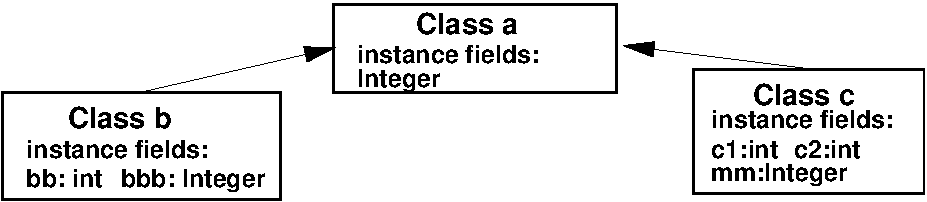
\includegraphics[scale=0.5]{umlex1}
    \label{fig:8i}
  }
  \qquad
  \subfloat[Pointers from permanent heap to transient heap]{
    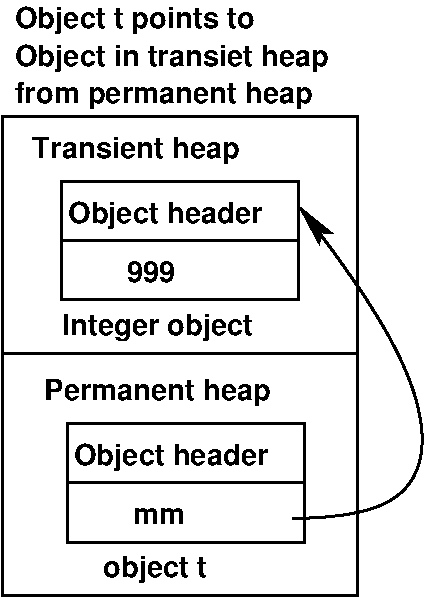
\includegraphics[scale=0.45]{ptp1}
    \label{fig:9a}
  }
  \qquad
  \subfloat[Points-to only in permanent heap]{
    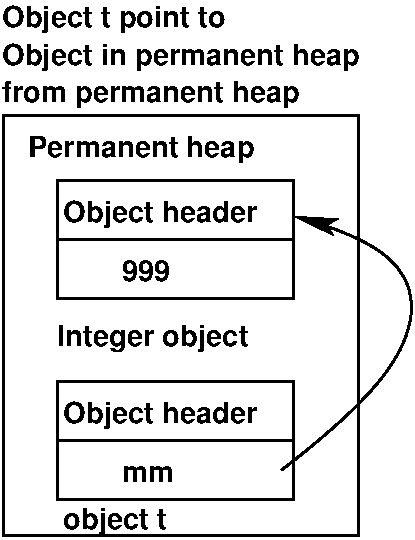
\includegraphics[scale=0.45]{ptp2}
    \label{fig:9b}
  }
  \caption{The UML representation of the class hierarchy used in
    Figure~\ref{fig:8} and the points-to problem}
  \label{fig:9}
\end{figure}


\newsavebox{\exinv}
\begin{lrbox}{\exinv}
  \begin{minipage}[b]{0.7\linewidth}
    \begin{Verbatim}[numbers=left,commandchars=\\\[\]]
private static Signal S;
public static void main(String args[]){
 Integer A = 0;\label[exinv:l1]
 Integer B = 1;\label[exinv:l2]
 S.setValue(A);\label[exinv:l3]
}
    \end{Verbatim}
  \end{minipage}
\end{lrbox}

\newsavebox{\exinvt}
\begin{lrbox}{\exinvt}
  \begin{minipage}[b]{0.7\linewidth}
    \begin{Verbatim}[numbers=left,commandchars=\\\[\]]
iconst_0 \label[exinvt:l0]
invokestatic  #2// valueOf:(I)Ljava/lang/Integer;\label[exinvt:l1]
astore_1 \label[exinvt:l2]     
iconst_1 \label[exinvt:l3]
invokestatic  #2// valueOf:(I)Ljava/lang/Integer;\label[exinvt:l4]
astore_2\label[exinvt:l5]
return        
    \end{Verbatim}
  \end{minipage}
\end{lrbox}

\newsavebox{\exinvtt}
\begin{lrbox}{\exinvtt}
  \begin{minipage}[b]{0.7\linewidth}
    \begin{Verbatim}[numbers=left,commandchars=\\\[\]]
new #3 // class java/lang/Integer\label[exinvtt:l1]
dup
iload_0
invokespecial #10 // Method "<init>":(I)V
areturn
    \end{Verbatim}
  \end{minipage}
\end{lrbox}

Given the class file(s), the data-flow analysis carried out is shown in
the flow-chart in Figure~\ref{fig:fanalysis}. The detailed algorithm for
each step is provided in~\cite{supp_amal02916}. Being a complex
procedure, we use simple code examples to describe the data-flow
analysis.

We divide the presentation of our data-flow analysis into two
sections. Section~\ref{sec:intra-proc-analys} presents the
\textit{Intra-procedural} data-flow analysis, which is complemented with
the \textit{Inter-procedural} data-flow analysis in
Section~\ref{sec:inter-proc-analys}.


\subsection{Intra-procedural analysis}
\label{sec:intra-proc-analys}

Figure~\ref{fig:8hc} shows a Java program as a call-graph. There are
three methods: \texttt{main}, \texttt{init}, and \texttt{MCall}. The
\texttt{main} method calls the \texttt{init} and the \texttt{MCall}
methods sequentially. The \texttt{init} method initializes a static
object reference \texttt{S} of type \texttt{Signal}. Figure~\ref{fig:8h}
shows the control-flow-graph (CFG) of the \texttt{MCall} method. It
consists of four basic blocks annotated as BB1, BB2, BB3, and BB4,
respectively. BB1 initializes objects \texttt{B} and \texttt{C}, whose
types \texttt{b} and \texttt{c} are inherited from a single parent class
\texttt{a} as shown in Figure~\ref{fig:8i}. Object \texttt{t} (BB1,
line~3) of type \texttt{a} is initialized to either type \texttt{b} or
\texttt{c} (BB2, line~2, BB3, line~3) depending upon the value of the
Boolean \texttt{a\_thread}. Finally, object \texttt{t} is emitted via
signal \texttt{S} (BB4, line~1).

\begin{compactitem}[-]

\item \underline{Step1} of the data-flow analysis algorithm starts by
  scanning the Java program for program points allocating signals (e.g.,
  method \texttt{init} in Figure~\ref{fig:8hc}). A globally accessible
  set $pp$ is defined, which holds all the program points allocating
  objects that will be placed in the permanent heap. Step1 scans the
  call graph from the starting program point (usually the \texttt{main}
  method) for signal allocation and places these program points into the
  set $pp$. Each individual tuple within the set $pp$ consists of one or
  more program points that allocate objects. After the scan phase, the
  set $pp$ holds $\{(5,\{\mathtt{init:BB1:1}\})\}$ for the example in
  Figure~\ref{fig:8hc}. The first element of the tuple gives the
  \textit{instance} size of the \texttt{Signal} class, the second
  element is the allocation program point~\footnote{The allocation
    program point is actually at the bytecode level, but in this paper
    we keep the program points at the Java source code level for ease of
    understanding.} for the example in Figure~\ref{fig:8hc}. If more
  than one signal is allocated, all these program points are placed in
  the set $pp$. Finally, Step2 is called to find all the signal emission
  program points.

\item \underline{Step2} is a recursive procedure that scans all
  reachable methods, in the call-graph, for the \texttt{setValue}
  virtual method call on the signal objects. These program points are
  placed in the set $PPC$ for each reachable method individually. For
  the example in Figure~\ref{fig:8}, this involves scanning method
  \texttt{MCall} and placing the program point: `BB4:line~1', in set
  $PPC$. Finally, Step3 of the algorithm is called to obtain all object
  allocation program points whose returned references are emitted via
  signals.
  
\item \underline{Step3} analyzes the emission expression for every
  program point in set $PPC$. An emitting expression can \textit{only}
  emit a method local variable or a field. Either Step4 or Step5 are
  called, depending on whether a field or a local variable is affected,
  respectively. In our current example a local variable (\texttt{t}) in
  Figure~\ref{fig:8h}, BB4, line~1, is being emitted (or formally called
  being affected) and hence, Step5 is called.
  
\item \underline{Step5} extracts the variable from the affected
  expression and calls Step7 for analysis. Step7 is the core of the
  whole data-flow analysis procedure that performs reachability analysis
  to identify the program points initializing the objects to be placed
  in the permanent heap. Before proceeding to Step7, let us assume that
  we have already obtained the correct program points from Step7 in set
  $alloc\_pps$. For our current example, given that the emitting program
  point is `BB4:line~1',
  $alloc\_pps = \{\mathtt{MCall:BB2:2}, \mathtt{MCall:BB3:3}\}$.
  Looking at Figure~\ref{fig:8h}, it is clear that object reference
  \texttt{t} can be initialized at either in BB2 line~2 or BB3 line~3,
  depending upon the value of variable \texttt{a\_thread} during program
  execution. For each of these program points, Step5 guarantees that the
  object reference does not \textit{escape} the lifetime of the
  method~\cite{choi1999escape}.~\footnote{Let $O$ be an object reference
    and $M$ be a method invocation. $O$ is said to escape $M$, if the
    lifetime of $O$ may exceed the lifetime of $M$.} If the object
  reference does not escape the lifetime of the method, then the
  algorithm checks if there are any reference fields within this
  object. If so, Step3 is invoked for migrating all object allocations,
  whose returned reference is held in these fields, into the permanent
  heap.

  Consider the program point in BB3 at line~3. Object \texttt{t} is
  initialized as class \texttt{c} (for program point in BB2 line~2,
  \texttt{t} is initialized and analyzed as class \texttt{b}), which has
  three fields (c.f. Figure~\ref{fig:8i}): two (\texttt{cc} and
  \texttt{ccc}) are primitive fields, but the third: \texttt{mm} is a
  reference field of type \texttt{Integer}. The \texttt{mm} reference
  field is initialized to an \texttt{Integer} object in BB3 line~4.
  Figure~\ref{fig:9a} shows the address held in \texttt{mm} if Step3 is
  not called from Step5. Reference field \texttt{mm} points to an object
  in transient heap space, which violates the first requirement in
  Section~\ref{sec:new-memory-model}. Calling Step3, guarantees that all
  potential \textit{pointed-to} objects from the permanent heap are also
  migrated to the permanent-heap. Note that Step3 and Step5 are mutually
  recursive and hence, perform a chained permanent heap migration. For
  the running example, the result of calling Step3 from Step5 is shown
  in Figure~\ref{fig:9b}.
  
  The final computation that Step5 performs is computing the size, which
  will be reserved in the permanent heap, of object \texttt{t}, given
  that $alloc\_pps$ may have multiple (two in our current example)
  elements. The primary idea is to reserve the maximum size from amongst
  all the different types being initialized. For the running example,
  \texttt{t} can be of type \texttt{b} or \texttt{c} during program
  execution. We compute the \textit{instance} size of both these types
  as 3 and 4 words, respectively~\footnote{According to Java semantics,
    all fields of a parent class are inherited by the children classes
    and hence, the sizes for \texttt{b} and \texttt{c} are 3 and 4
    words, respectively.} and reserve 4 words (plus object header size)
  in the permanent heap space. Step7 returns multiple program points in
  set $alloc\_pps$ if and only if these program points are mutually
  unreachable. This, guarantees that the reserved permanent heap space
  can be \textit{reused} at runtime by all program points in set
  $alloc\_pps$.  \newline
  \begin{compactitem}[$\bullet$]
  \item \textbf{Design decision}: We have disallowed method local object
    references from escaping as a trade-off between space utilization
    and functional correctness. If we allow, for example \texttt{t} in
    Figure~\ref{fig:8h}, to escape method \texttt{MCall}, then any of
    the reference fields of \texttt{t} (e.g., \texttt{mm}) might be
    reinitialized at some other program point. This new program point
    would also then need to be considered and space on the permanent
    heap would need to be reserved for the object allocation. This can
    result in the permanent heap becoming too large. Conversely, if the
    escape analysis is not performed, then there will be pointers
    pointing from the permanent heap to transient heap, which may result
    in potentially incorrect program behavior. Simply not allowing any
    object reference to exceed the lifetime of the method avoids both
    these problems.
  \end{compactitem}
  
\item \underline{Step7}, given a program point that affects a variable
  (also termed the \textit{use} program point) gives one or more program
  points initializing that variable (also called the defining program
  point). Step7 first builds the standard \textit{use-def}
  chains~\cite{steven1997advanced} to obtain the program points defining
  the variable. If the defining program points are \texttt{new} or
  \texttt{newarray} bytecodes~\cite{meyer1997java}, then these program
  points are simply unioned into the set of program points that will be
  returned by this function. If the defining program points are
  themselves affecting variables, then Step7 is called recursively to
  follow the so called deferred program edges~\cite{burke1995flow} to
  finally reach one or more program points that allocates the object or
  if the variable is not initialized then gives a compile time
  \texttt{not initialized} error. Note, that this amounts to carrying
  out a complete alias analysis. If the defining program point affects a
  field, then Step4 is called, which calls Step7 via Step6, we describe
  Step4 and Step6 in the next section. If the defining program point is
  anything but any of the aforementioned statements, then an error is
  raised, stating that the variable might be initialized outside the
  method being analyzed. Finally, Step7 makes sure that the program
  points being returned are not reachable from each other.\newline
  \begin{compactitem}[$\bullet$]
  \item \textbf{Design decision}: We have consciously decided to not
    allow object allocation outside the method that uses that object in
    Step7. The objective of our data-flow algorithm is to identify all
    the program points that allocate objects whose returned references
    are emitted as signal values. We are performing compile time memory
    allocation, which, as we will see later, requires us to replace the
    \texttt{new} and \texttt{newarray} bytecodes with a different set of
    bytecodes (c.f. Section~\ref{sec:prod-back-code}). We cannot blindly
    replace these bytecodes in methods other than the ones being
    analyzed, because, consequently \textit{any} other program point,
    related or unrelated to signals, using the same object
    initialization program point would overwrite the object value as it
    inadvertently shares the same object. A simple example elucidating
    the situation is shown in Figure~\ref{fig:10}.
    
    In Figure~\ref{fig:10a}, we initialize two \texttt{Integer} object
    type variables; \texttt{A} and \texttt{B} to constant \texttt{int}
    values. Then we emit \texttt{A} via signal \texttt{S}. The bytecode
    produced from this Java program is shown in
    Figure~\ref{fig:10b}. First, the constant 0 is loaded onto the stack
    and the method \texttt{valueOf} in the \texttt{Integer} class, from
    the Java standard library, is invoked, which allocates memory and
    initializes the returned reference field to 0, the returned
    reference is then stored on the stack
    (lines~\ref{exinvt:l0}-\ref{exinvt:l2}), same is done for the object
    \texttt{B} in lines~\ref{exinvt:l3}-\ref{exinvt:l5}. The actual
    object initialization is carried out inside the \texttt{valueOf}
    method, Figure~\ref{fig:10c}, line~\ref{exinvtt:l1}. If we were to
    replace this \texttt{new} bytecode, to point to some memory words in
    the permanent heap, then both; \texttt{A} and \texttt{B} will point
    to the same place in permanent heap. Consequently, first a constant
    0 will be written in the allocated memory (Figure~\ref{fig:10b},
    line~\ref{exinvt:l2}) and then this value will be overwritten to 1
    (Figure~\ref{fig:10b}, line~\ref{exinvt:l4}), resulting in
    functionally incorrect code. The \textit{only} solution to this
    problem is to \textit{inline} the called method, \texttt{valueOf} in
    this case. But, extreme caution is required when in-lining methods,
    because the method might be too large to fit in the method cache, or
    more than one such methods might need to be in-lined (in case a
    method itself calls another method, which does the actual object
    allocation and so on and so forth). To put the cache size
    restriction into perspective, all our benchmarks have a very limited
    cache size of only 1KB. Thus, we have decided to disallow, object
    allocation outside of the method being analyzed.  As a consequence
    of this design decision, the SystemJ programmer now needs to make
    explicit deep copies as shown in Figure~\ref{fig:8h} BB2 line~3 and
    BB3 line~4.
  \end{compactitem}

\begin{figure}[t!]
  \centering
  \subfloat[Example Java code snippet]{
    \scalebox{0.6}{\usebox{\exinv}}
    \label{fig:10a}
  }
  \qquad
  \subfloat[Produced Java bytecode]{
    \scalebox{0.6}{\usebox{\exinvt}}
    \label{fig:10b}
  }
  \qquad
  \subfloat[The bytecode for method \texttt{valueOf} in Integer class]{
    \scalebox{0.6}{\usebox{\exinvtt}}
    \label{fig:10c}
  }
  \caption{Inadvertent object sharing problem}
  \label{fig:10}
\end{figure}

\end{compactitem}

  
\subsection{Inter-procedural analysis}
\label{sec:inter-proc-analys}

Until now we have only described those parts of our data-flow analysis
that handle local method references being emitted via signals. Step4 and
Step6 (c.f. Figure~\ref{fig:fanalysis}) described in this section work
in conjunction with the previously described steps in order to handle
cases where Java field references may be affected by signal
emissions. We again use a simple example shown in Figure~\ref{fig:8j} to
describe Step4 and Step6 of our data-flow analysis.

\begin{figure}[t!]
  \centering
  \scalebox{0.6}{% Graphic for TeX using PGF
% Title: D:\jpaper\Interproc.dia
% Creator: Dia v0.97.2
% CreationDate: Wed May 13 15:25:05 2015
% For: amal029
% \usepackage{tikz}
% The following commands are not supported in PSTricks at present
% We define them conditionally, so when they are implemented,
% this pgf file will use them.
\ifx\du\undefined
  \newlength{\du}
\fi
\setlength{\du}{15\unitlength}
\begin{tikzpicture}
\pgftransformxscale{1.000000}
\pgftransformyscale{-1.000000}
\definecolor{dialinecolor}{rgb}{0.000000, 0.000000, 0.000000}
\pgfsetstrokecolor{dialinecolor}
\definecolor{dialinecolor}{rgb}{1.000000, 1.000000, 1.000000}
\pgfsetfillcolor{dialinecolor}
\definecolor{dialinecolor}{rgb}{1.000000, 1.000000, 1.000000}
\pgfsetfillcolor{dialinecolor}
\fill (24.195000\du,-24.005000\du)--(24.195000\du,-19.650000\du)--(36.650000\du,-19.650000\du)--(36.650000\du,-24.005000\du)--cycle;
\pgfsetlinewidth{0.100000\du}
\pgfsetdash{}{0pt}
\pgfsetdash{}{0pt}
\pgfsetmiterjoin
\definecolor{dialinecolor}{rgb}{0.000000, 0.000000, 0.000000}
\pgfsetstrokecolor{dialinecolor}
\draw (24.195000\du,-24.005000\du)--(24.195000\du,-19.650000\du)--(36.650000\du,-19.650000\du)--(36.650000\du,-24.005000\du)--cycle;
% setfont left to latex
\definecolor{dialinecolor}{rgb}{0.000000, 0.000000, 0.000000}
\pgfsetstrokecolor{dialinecolor}
\node at (30.422500\du,-21.632500\du){};
\definecolor{dialinecolor}{rgb}{1.000000, 1.000000, 1.000000}
\pgfsetfillcolor{dialinecolor}
\fill (24.650000\du,-31.250000\du)--(24.650000\du,-25.250000\du)--(36.200000\du,-25.250000\du)--(36.200000\du,-31.250000\du)--cycle;
\pgfsetlinewidth{0.100000\du}
\pgfsetdash{}{0pt}
\pgfsetdash{}{0pt}
\pgfsetmiterjoin
\definecolor{dialinecolor}{rgb}{0.000000, 0.000000, 0.000000}
\pgfsetstrokecolor{dialinecolor}
\draw (24.650000\du,-31.250000\du)--(24.650000\du,-25.250000\du)--(36.200000\du,-25.250000\du)--(36.200000\du,-31.250000\du)--cycle;
% setfont left to latex
\definecolor{dialinecolor}{rgb}{0.000000, 0.000000, 0.000000}
\pgfsetstrokecolor{dialinecolor}
\node at (30.425000\du,-28.055000\du){};
\definecolor{dialinecolor}{rgb}{1.000000, 1.000000, 1.000000}
\pgfsetfillcolor{dialinecolor}
\fill (25.087500\du,-30.550000\du)--(25.087500\du,-27.050000\du)--(35.812500\du,-27.050000\du)--(35.812500\du,-30.550000\du)--cycle;
\pgfsetlinewidth{0.100000\du}
\pgfsetdash{}{0pt}
\pgfsetdash{}{0pt}
\pgfsetmiterjoin
\definecolor{dialinecolor}{rgb}{0.000000, 0.000000, 0.000000}
\pgfsetstrokecolor{dialinecolor}
\draw (25.087500\du,-30.550000\du)--(25.087500\du,-27.050000\du)--(35.812500\du,-27.050000\du)--(35.812500\du,-30.550000\du)--cycle;
% setfont left to latex
\definecolor{dialinecolor}{rgb}{0.000000, 0.000000, 0.000000}
\pgfsetstrokecolor{dialinecolor}
\node[anchor=west] at (25.537500\du,-29.405000\du){1: A = new a();};
% setfont left to latex
\definecolor{dialinecolor}{rgb}{0.000000, 0.000000, 0.000000}
\pgfsetstrokecolor{dialinecolor}
\node[anchor=west] at (25.537500\du,-28.605000\du){2: A.b = new Integer(70);};
% setfont left to latex
\definecolor{dialinecolor}{rgb}{0.000000, 0.000000, 0.000000}
\pgfsetstrokecolor{dialinecolor}
\node[anchor=west] at (25.537500\du,-27.805000\du){3: MCall1();};
% setfont left to latex
\definecolor{dialinecolor}{rgb}{0.000000, 0.000000, 0.000000}
\pgfsetstrokecolor{dialinecolor}
\node[anchor=west] at (24.950000\du,-31.550000\du){main method};
\definecolor{dialinecolor}{rgb}{1.000000, 1.000000, 1.000000}
\pgfsetfillcolor{dialinecolor}
\fill (24.567500\du,-23.005000\du)--(24.567500\du,-21.105000\du)--(36.447500\du,-21.105000\du)--(36.447500\du,-23.005000\du)--cycle;
\pgfsetlinewidth{0.100000\du}
\pgfsetdash{}{0pt}
\pgfsetdash{}{0pt}
\pgfsetmiterjoin
\definecolor{dialinecolor}{rgb}{0.000000, 0.000000, 0.000000}
\pgfsetstrokecolor{dialinecolor}
\draw (24.567500\du,-23.005000\du)--(24.567500\du,-21.105000\du)--(36.447500\du,-21.105000\du)--(36.447500\du,-23.005000\du)--cycle;
% setfont left to latex
\definecolor{dialinecolor}{rgb}{0.000000, 0.000000, 0.000000}
\pgfsetstrokecolor{dialinecolor}
\node[anchor=west] at (25.017500\du,-21.860000\du){1: S.setValue(A);};
% setfont left to latex
\definecolor{dialinecolor}{rgb}{0.000000, 0.000000, 0.000000}
\pgfsetstrokecolor{dialinecolor}
\node[anchor=west] at (31.195000\du,-18.845000\du){MCall1 method};
\pgfsetlinewidth{0.100000\du}
\pgfsetdash{}{0pt}
\pgfsetdash{}{0pt}
\pgfsetbuttcap
{
\definecolor{dialinecolor}{rgb}{0.000000, 0.000000, 0.000000}
\pgfsetfillcolor{dialinecolor}
% was here!!!
\pgfsetarrowsend{stealth}
\definecolor{dialinecolor}{rgb}{0.000000, 0.000000, 0.000000}
\pgfsetstrokecolor{dialinecolor}
\draw (30.450000\du,-27.050000\du)--(30.507500\du,-23.005000\du);
}
\pgfsetlinewidth{0.100000\du}
\pgfsetdash{{1.000000\du}{1.000000\du}}{0\du}
\pgfsetdash{{1.000000\du}{1.000000\du}}{0\du}
\pgfsetmiterjoin
\pgfsetbuttcap
{
\definecolor{dialinecolor}{rgb}{0.000000, 0.000000, 0.000000}
\pgfsetfillcolor{dialinecolor}
% was here!!!
\pgfsetarrowsend{stealth}
{\pgfsetcornersarced{\pgfpoint{0.000000\du}{0.000000\du}}\definecolor{dialinecolor}{rgb}{0.000000, 0.000000, 0.000000}
\pgfsetstrokecolor{dialinecolor}
\draw (24.567500\du,-22.055000\du)--(23.517500\du,-22.055000\du)--(23.517500\du,-29.675000\du)--(25.087500\du,-29.675000\du);
}}
% setfont left to latex
\definecolor{dialinecolor}{rgb}{0.000000, 0.000000, 0.000000}
\pgfsetstrokecolor{dialinecolor}
\node[anchor=west] at (20.245000\du,-24.280000\du){Allocated in BB1 line 1};
% setfont left to latex
\definecolor{dialinecolor}{rgb}{0.000000, 0.000000, 0.000000}
\pgfsetstrokecolor{dialinecolor}
\node[anchor=west] at (25.195000\du,-26.080000\du){BB1};
% setfont left to latex
\definecolor{dialinecolor}{rgb}{0.000000, 0.000000, 0.000000}
\pgfsetstrokecolor{dialinecolor}
\node[anchor=west] at (24.545000\du,-20.330000\du){BB2};
\end{tikzpicture}
}
  \caption{Inter-procedural analysis with fields. \texttt{A} and
    \texttt{S} are static fields}
  \label{fig:8j}
\end{figure}

\begin{compactitem}[-]

\item \underline{Step4} is the dual of Step5. It works on Java fields
  rather than method local variables like Step5. The other difference
  between the two is that Step5 calls Step7 via Step6, which performs
  inter-procedural analysis.

\item \underline{Step6} can be conceptually partitioned into two
  parts. Part-1 returns the program points allocating objects within the
  same method that the field is being used. The more interesting part is
  part-2, which carries out \textit{inter-procedural} analysis if the
  affected field being analyzed is not allocated in the same method. 

  Let us consider the Java program call-graph in Figure~\ref{fig:8j} to
  explain the inter-procedural analysis. The \texttt{main} method
  initializes two objects: \texttt{A}, a static field, of type
  \texttt{a} (c.f. Figure~\ref{fig:8i}) and its \texttt{Integer} type
  reference field \texttt{b}. Next, \texttt{main} calls method
  \texttt{MCall1}. Field \texttt{A} is emitted via signal \texttt{S} in
  method \texttt{MCall1}. Our data-flow analysis algorithm needs to
  locate the program points in BB1 lines~1 and 2, so that these object
  allocations can be moved to the permanent heap space.

  Part-1 of Step6 calls Step7 passing it method \texttt{MCall1} to find
  out the object \texttt{A} and its field's allocation program
  points. Step7 being an \textit{intra-procedural} analysis step returns
  back an empty list ($alloc\_pps = \emptyset$). In such a case, Step6
  looks up the call-graph tree to find out the caller methods for the
  current callee, this lookup procedure also includes looking up all the
  potential callers indicated by the GRC-analysis
  (c.f. Section~\ref{sec:agrc-analysis}). Once the caller method is
  identified in the call-graph, Step6 recursively calls itself to
  analyze the caller. This procedure is continued until the program
  point allocating the affected field is identified or the analysis
  reaches the top of the call graph, in the latter case a \texttt{Not
    initialized field} error is thrown by the compiler. In case of
  Figure~\ref{fig:8j}, there is a single caller: the \texttt{main}
  method in the call-graph for callee \texttt{MCall1}, which is analyzed
  to find the program point allocating field \texttt{A}, this program
  point is returned by Step6. Note that multiple callers might call the
  same callee, due to \textit{may} happen before results produced by the
  GRC-analysis. In such cases, all the callers need to be analyzed in
  order to identify the program points allocating the affected field and
  to make sure that such allocations exist in all paths, else, the field
  would be uninitialized in some run of the SystemJ program.
\end{compactitem}

This finishes the treatment of the data-flow analysis algorithm to
identify the program points that return an object allocation reference,
which may be emitted via signals. Now that we have identified these
program points, we next give the procedure to generate the back-end code
that: (1) replaces the object allocation bytecodes with time predictable
alternatives and (2) performs compile time memory allocation in the
permanent heap space.

\section{Back-end code generation}
\label{sec:prod-back-code}

\newsavebox{\baone}
\begin{lrbox}{\baone}
  \begin{minipage}[b]{0.5\linewidth}
    \begin{algo}
      \SetKwData{Let}{let}
      \SetKwFunction{Steptwo}{Step2}
      \SetKwFunction{SortDescending}{sortUniqueDescending}
      \SetKwFunction{Load}{load}
      \SetKwFunction{ReplaceByteCode}{replaceByteCode}
      \KwIn{maxMem: Maximum memory address} 
      \tcc*[h]{$defs$ is the same set as $pp$ in Figure~\ref{fig:fanalysis}}\\
      \KwIn{$defs$: The program points to replace} 
      \KwIn{$program$: The program} 
      \BlankLine
      \Let $allocPtr \leftarrow$ maxMem\;
      \Let $header\_size \leftarrow 2$\;
      \ForEach{$(size,dd) \in defs$} {
        \Let $dd \leftarrow$ \SortDescending($dd$)\;
        \Let $M \leftarrow$ \Load($dd$)\;
        \Let $allocPtr \leftarrow allocPtr - (size + header\_size)$\;\label{baone:l1}
        \lIf {$allocPtr < 0$} {\texttt{raise No\_mem}}\;\label{baone:l2}
        \ForEach {$d \in dd$} {
          \ReplaceByteCode($allocPtr,d,M,size)$\;
        }
      }
    \end{algo}
  \end{minipage}
\end{lrbox}

\newsavebox{\batwo}
\begin{lrbox}{\batwo}
  \begin{minipage}[b]{0.5\linewidth}
    \begin{algo}
      \KwIn{$allocPtr$: allocation pointer}
      \KwIn{pp: program point to replace} 
      \KwIn{$M$: Method containing the program point} 
      \KwIn{$size$: Size of the allocated object/array} 
      \SetKwData{Let}{let}
      \SetKwData{GetArg}{getArg}
      \SetKwData{ReplaceNew}{replaceNew}
      \SetKwData{ReplaceNewA}{replaceNewArrayB}
      \SetKwData{ReplaceNewAA}{replaceNewArrayO}
      \SetKwData{AdjConditionals}{adjustConditionals}
      \BlankLine
      \uIf {$pp = \mathtt{new}$} {
        \Let $arg \leftarrow$ \GetArg($pp$)\;
        \ReplaceNew($pp$,$M$,$arg$,$size$)\;\label{batwo:l1}
        \AdjConditionals($M$,31)\;
      }
      \uElseIf {$pp = \mathtt{newarray}$} {
        \Let $arg \leftarrow$ \GetArg($pp$)\;
        \uIf {$arg = \mathtt{primitive}$} {
          \ReplaceNewA($pp$,$M$,$arg$,$size$)\;\label{batwo:l2}
        }\lElse {
          \ReplaceNewAA($pp$,$M$,$arg$,$size$)\;\label{batwo:l3}
        }
        \AdjConditionals($M$,31)\;\label{batwo:l4}
      }
      \lElse {\texttt{raise error}}
    \end{algo}
  \end{minipage}
\end{lrbox}

The back-end code generation is a two step-procedure as shown in
Figures~\ref{fig:11a} and~\ref{fig:11b}, respectively. The memory
allocation algorithm (Figure~\ref{fig:11a}) takes as input the maximum
memory address, the program points to replace and the whole program
itself as input. Two variables: $allocPtr$ and $header\_size$ are
initialized to the maximum memory address and the constant two,
respectively. The $allocPtr$ is decremented by the size of the object to
be allocated (obtained from the data-flow analysis algorithm,
Figure~\ref{fig:fanalysis}) plus, the object header size
(line~\ref{baone:l1}) -- this simple \textit{bumping} of the allocation
pointer is termed bump pointer memory allocation. If the resultant
$allocPtr$ value is less than 0, then we have exhausted total permanent
memory allocation and correspondingly an error is raised
(line~\ref{baone:l2}). If there is enough memory available then, the
object allocation bytecode at the program point is replaced by
alternative bytecodes in the second step, shown in Figure~\ref{fig:11b}.

\begin{figure}[t!]
  \centering
  \subfloat[Bump-pointer memory allocation] {
    \scalebox{0.9}{\usebox{\baone}}
    \label{fig:11a}
  }
  \qquad
  \subfloat[Replacing the \texttt{new}, \texttt{newarray}, and
  \texttt{anewarray} bytecodes] { \scalebox{0.9}{\usebox{\batwo}}
    \label{fig:11b}
  }
  \caption{The back-end code generation pseudo-algorithm}
  \label{fig:11}
\end{figure}


{\color{red} The algorithm (Figure~\ref{fig:11b}) used to replace the
  object allocation bytecodes takes as input four arguments: the
  allocation pointer, $allocPtr$, the program point to replace $pp$, and
  the method containing the program point: $M$ and the size to
  allocate. }There are \textit{three} types of bytecodes in the JVM
specification: (1) the \texttt{new} bytecode that allocates an
object. (2) The \texttt{newarray} bytecode that allocates arrays holding
primitives, and (3) \texttt{anewarray} bytecode that allocates arrays
holding references. This distinction is important since the number of
bytes used to represent each of these bytecodes differ. The \texttt{new}
and \texttt{anewarray} bytecodes are encoded in the class file with
three bytes, whereas the \texttt{newarray} bytecode only uses two bytes
in the class file representation.

Different methods are called to replace each of these allocation
variants: Figure~\ref{fig:11b}, line~\ref{batwo:l1} replacing
\texttt{new}, line~\ref{batwo:l2} replacing \texttt{newarray}, and
line~\ref{batwo:l3} replacing \texttt{anewarray} bytecodes,
respectively. All methods have the same logic, except that some padding
(represented as \texttt{nop} bytecodes) is needed in case of the
\texttt{newarray} and \texttt{anewarray} bytecodes. This padding is
needed to correctly update the conditional instruction's target address
after replacement (line~\ref{batwo:l4}).

All conditional instruction's, following the object allocation
bytecodes, target addresses need to be incremented by {\color{red} 31}
bytes after replacement. This {\color{red} 31} byte increment is made
obvious by Figures~\ref{fig:11c} and~\ref{fig:11d}, which show the Java
bytecode snippets for the example program in Figure~\ref{fig:8j} before
and after \texttt{new} bytecode replacement, respectively\footnote{In
  both these figures, the line numbers are shown on the right of the
  program. The numbers adjacent to the bytecodes are the starting bytes
  for each of the bytecodes as obtained by the \texttt{javap -c -v}
  command}. Figure~\ref{fig:11c} shows the bytecode produced by the Java
compiler for the \texttt{A} object allocation in the \texttt{main}
method. The very first bytecode, \texttt{new}, takes as argument the
index, \texttt{2}, into the constant pool that holds the type of object
to allocate. The returned object reference is then duplicated
(\texttt{dup} instruction). Next, the constructor of the class
\texttt{a} is invoked to initialize the returned reference and finally,
the returned reference is put into a static field of the class. The
\texttt{new} bytecode is timing \textit{unpredictable}, because it might
invoke the GC, which has an unbounded collection cycle. It might also
generate a runtime out of memory exception, thereby violating safety
criticality. We replace this \texttt{new} bytecode with safe and time
predictable bytecodes as shown in Figure~\ref{fig:11d}.

\newsavebox{\bone}
\begin{lrbox}{\bone}
  \begin{minipage}[b]{0.7\linewidth}
    \begin{Verbatim}[numbers=right,commandchars=\\\[\]]
--- constant-pool snippet ----
#2 = Class     #79     //a/a
#3 = Methodref #2.#78  //a/a.''<init>'':()V
#4 = Fieldref  #12.#80 //test/test.A:La/a;
---------- main method snippet --------
0:new #2           // class a/a
3:dup
4:invokespecial #3 // Method a/a.''<init>'':()V
7:putstatic     #4 // Field A:La/a;
    \end{Verbatim}
  \end{minipage}
\end{lrbox}

\newsavebox{\btwo}
\begin{lrbox}{\btwo}
  \begin{minipage}[b]{0.7\linewidth}
    \begin{Verbatim}[numbers=right,commandchars=\\\[\]]
--- constant-pool snippet ----
#2 = Class     #79     //a/a
#3 = Methodref #2.#78  //a/a.''<init>'':()V
#4 = Fieldref  #12.#80 //test/test.A:La/a;
.... //other constants
#154 = Integer            65483
#155 = Integer            65485
---------- main method snippet --------
 0:ldc_w         #154 // int 65483\label[btwo:l1]
 3:dup 
 4:ldc_w         #155 // int 65485\label[btwo:l3]
 7:swap
 8:invokestatic  #151 // Method Native.wr:(II)V\label[btwo:l4]
11:dup\label[btwo:l5]
12:bipush        1
14:iadd
15:ldc_w         #2   // class a/a
18:bipush        5
20:iadd
21:swap
22:invokestatic  #151 // Method Native.wr:(II)V\label[btwo:l2]\label[btwo:l6]
25:ldc_w         #155 // start of fields\label[btwo:l7]\label[btwo:l8]
28:ldc_w         #156 // size of the object
31:invokestatic  #150 // Method Native.wrl:(II)V\label[btwo:l9]\label[btwo:l10]
34:dup
35:invokespecial #3   // Method a/a.''<init>'':()V
38:putstatic     #4   // Field A:La/a;
    \end{Verbatim}
  \end{minipage}
\end{lrbox}

\begin{figure}[t!]
  \centering
  \subfloat[Java bytecode snippet and class constant-pool for example in
  Figure~\ref{fig:8j}]{
    \scalebox{0.65}{\usebox{\bone}}
    \label{fig:11c}
  }
  \qquad
  \subfloat[Java bytecode snippet and class constant-pool for example in
  Figure~\ref{fig:8j} after \texttt{new} bytecode replacement]{
    \scalebox{0.65}{\usebox{\btwo}}
    \label{fig:11d}
  }

  \subfloat[Java object allocation in permanent heap]{
    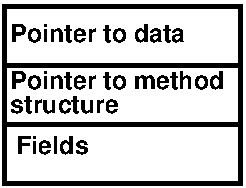
\includegraphics[scale=0.5]{oalloc}
    \label{fig:11e}
  }
  \qquad\qquad
  \subfloat[Java (2x2x2) array allocation in permanent heap]{
    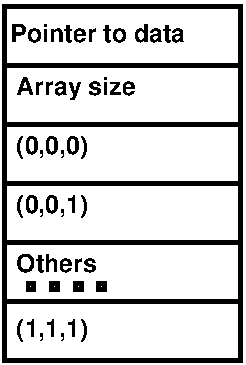
\includegraphics[scale=0.5]{aalloc}
    \label{fig:11f}
  }
  \caption{The back-end generated code and compacted object
    representation in heap}
  \label{fig:15}
\end{figure}

A single \texttt{new} bytecode (consuming 3 bytes in the class file) is
replaced with a list of bytecodes in lines~\ref{btwo:l1}-\ref{btwo:l2}
(line numbers are given on the right) consuming {\color{red} 34} bytes
in the class file, hence the {\color{red} 31} byte increment of target
addresses of the conditional bytecodes. The core idea is very simple;
since we have already allocated memory for the object
(Figure~\ref{fig:11a}), we can simply replace the \texttt{new} bytecode
with a bytecode that loads the allocation pointer ($allocPtr$) onto the
stack (line~\ref{btwo:l1}) as the object reference. The rest of the
bytecodes setup the object header for the allocated object. Our object
header is two words (the object structure for the running example is
shown in Figure~\ref{fig:11e}), the first word contains the pointer to
the start of data, in the current example it is the address 65485. The
first word of the object header is initialized in
lines~\ref{btwo:l3}-\ref{btwo:l4} in Figure~\ref{fig:11d}. The second
word of the object header is the pointer to the start of the method
structure of the class (c.f. Figure~\ref{fig:6b}). The second word of
the object header is initialized in lines~\ref{btwo:l5}-\ref{btwo:l6} in
Figure~\ref{fig:11d}. {Finally, the fields of the object are zeroed, on
  lines~\ref{btwo:l7}-\ref{btwo:l9}. The method \texttt{Native.wrl}
  takes as input the start address of the object's fields and the size
  of the object as the arguments and writes zeros in these memory
  words.}


In case of \texttt{newarray} and \texttt{anewarray} bytecodes, the array
layout (shown in Figure~\ref{fig:11f}) differs from standard real-time
JVM implementations. For array allocation, we again use a 2 word object
header. The first word contains the pointer to the start of array
data. The second word of the object header contains the size of the
array. Other than the smaller object header size compared to standard
real-time JVM object header size (usually 8 words), which uses
spines~\cite{pizlo2010schism} or handles~\cite{msch05} for arrays and
regular objects, respectively, we also structure our arrays
differently. We have decided to place arrays in a row major order and
contiguously irrespective of the array dimensions (as in `C') rather
than using linked lists for array traversal in order to allow $O(1)$
array accesses.

\section{Experimental results}
\label{sec:experimental-results}

We have carried out two sets of experiments: (a) micro-benchmarks and
(b) static WCRT analysis on well established real-time benchmarks to
study the efficacy of the proposed memory management scheme compared to:
(1) two different real-time garbage collector (RTGC)
implementations~\cite{msch05,ipat13} and (2) The \textit{Safety Critical
  Java} (SCJ)~\cite{scj2013} implementation on the JOP platform. The
first RTGC framework is the one proposed in~\cite{msch05}, which is a
concurrent version of Cheney's copy collector developed by
Baker~\cite{baker1978list}. In the rest of the section we call it
JOP-GC. The second one proposed in~\cite{ipat13} is a variation of the
real-time collector described in~\cite{pizlo2010schism}, in the rest of
the section we call it AGC. The SCJ framework on the other hand is a GC
less Java specification, designed to build hard real-time safety
critical applications. All our micro-benchmark experiments are run in
ModelSim, simulating the real-time hardware implemented JVM called JOP,
running at 100 MHz, with 256KB of main memory, 1KB of method cache, and
4KB of stack cache.

\subsection{Micro benchmarks}
\label{sec:micro-benchmarks}

We experiment with three micro-benchmarks: (1) simple object allocation,
where we allocate, in a tight loop, 2 objects with 1 word primitive
field each. (2) Simple array allocation, where we allocate, in a tight
loop, an object with an array type reference field, which is itself
initialized to a 20 word 1D array of primitive \texttt{int} type. (3)
Complex object allocation: in this case, we use a nested 2D loop. In
every outer loop iteration, a \textit{reference} type 1D array of size
20 is allocated. In every iteration of the inner loop, 2 objects are
allocated and the second object's reference is set as the array value.
The example benchmarks are available from~\cite{ipat13}.

\begin{figure}[t!]
  \centering
  \subfloat[Simple object memory allocation runtime without GC
  invocation.]{
    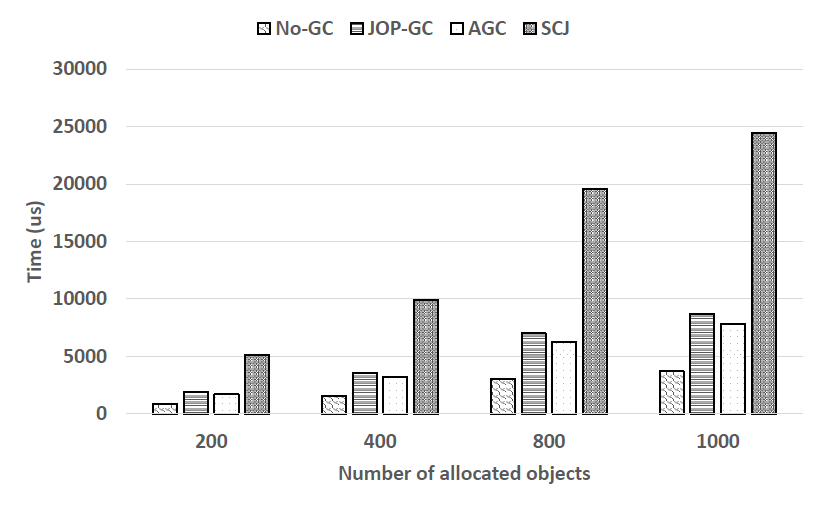
\includegraphics[scale=0.29]{soruntime.PNG}
    \label{fig:12a}
  }
  \qquad
  \subfloat[Simple array memory allocation runtime without GC
  invocation.]{
    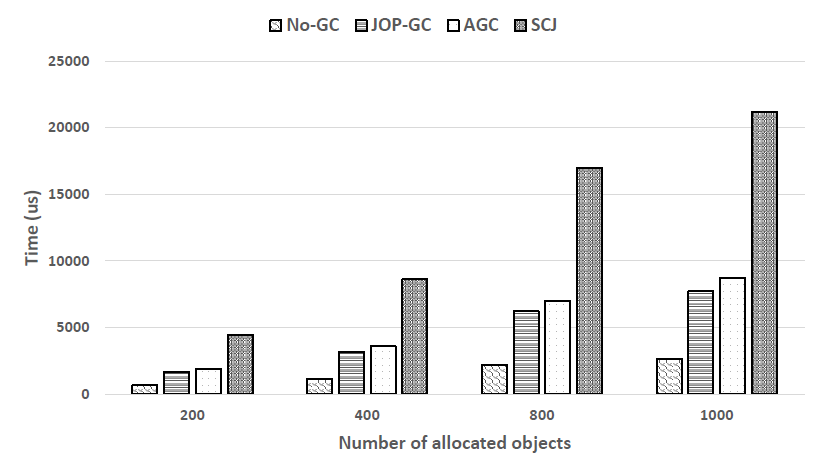
\includegraphics[scale=0.29]{aoruntime.PNG}
    \label{fig:12c}
  }
  \qquad
  \subfloat[Complex object memory allocation runtime without GC
  invocation.]{
    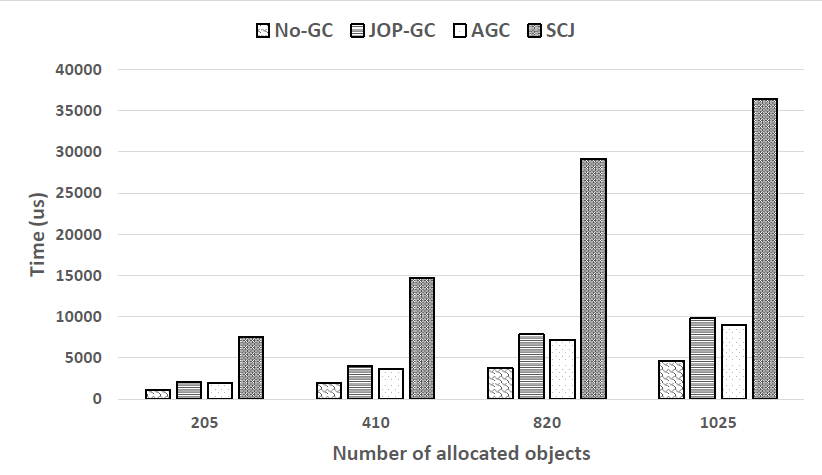
\includegraphics[scale=0.29]{coruntime.PNG}
    \label{fig:12e}
  }
  \caption{Runtime for micro-benchmarks without GC invocation.}
  \label{fig:12}
\end{figure}

\begin{figure}[t!]
  \centering
  \subfloat[Simple object memory allocation runtime with possible
  GC. \textbf{N/P} stands for \texttt{NullPointer} exception]{
    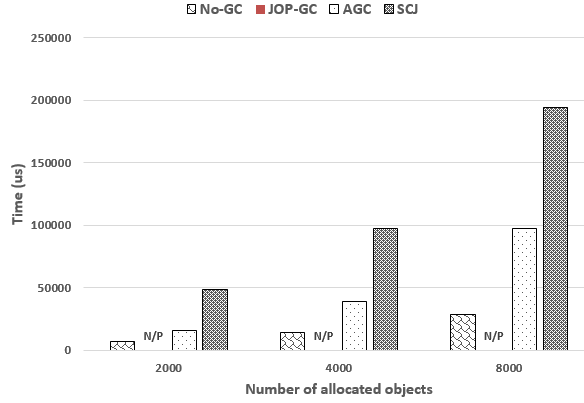
\includegraphics[scale=0.4]{sogruntime.PNG}
    \label{fig:12b}
  }
  \qquad
  \subfloat[Simple array memory allocation runtime with possible GC
  invocation. \textbf{N/P} stands for \texttt{NullPointer} exception]{
    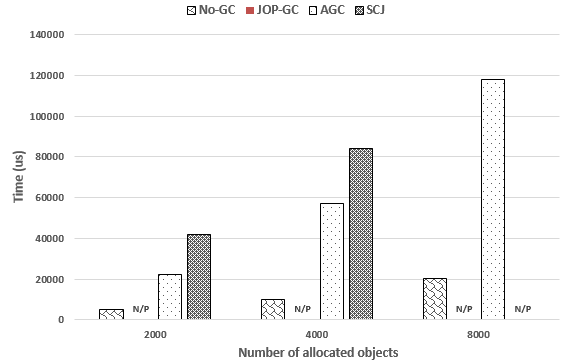
\includegraphics[scale=0.4]{aogruntime.PNG}
    \label{fig:12d}
  }
  \qquad
  \subfloat[Complex object memory allocation runtime with possible GC
  invocation. \textbf{N/P} stands for \texttt{NullPointer} exception]{
    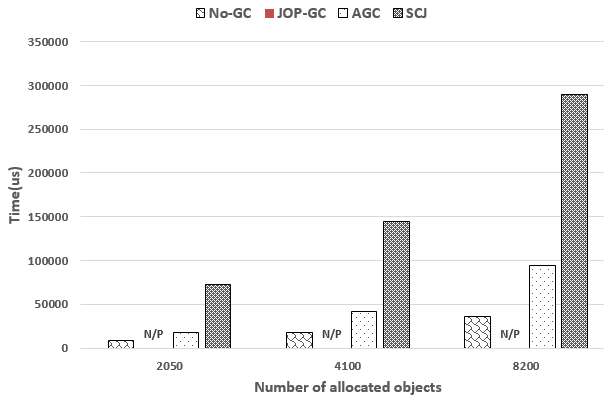
\includegraphics[scale=0.4]{cogruntime.PNG}
    \label{fig:12f}
  }
  \caption{Runtime for micro-benchmarks with possibility of GC
    invocation}
  \label{fig:16}
\end{figure}

The runtime comparison between the four approaches for each of the
micro-benchmarks is shown in Figures~\ref{fig:12}
and~\ref{fig:16}. Figures~\ref{fig:12} and~\ref{fig:16} give the
execution times for completion of a memory allocation request in two
cases: (1) when the GC is not invoked, i.e., there is enough memory
available to allocate the requested memory and (2) when the GC is
invoked to collect the garbage when enough memory is not available upon
a memory allocation request from the mutator, respectively. The proposed
approach is, on average, approximately 3$\times$ faster compared to the
RTGC based approaches. In many cases (see Figure~\ref{fig:16}) JOP-GC
could not perform garbage collection correctly, as it ran out of handles
resulting in \texttt{NullPointer} exceptions. There is a greater speedup
in case of array allocations compared to simple object allocations. The
runtime memory allocation time difference is significant in the case of
GC invocation when compared to the case of no GC invocation.

SCJ specification prohibits GC~\cite{scj2013} and divides the memory
organization into regions such as immortal memory and scoped memory,
similar to the permanent and transient heap spaces described in this
paper. Given this similarity in the memory organization schemes, we
expected to observe memory allocation times, for SCJ, similar to those
obtained in the No-GC approach proposed in this paper. Yet, as we see
from Figures~\ref{fig:12} and \ref{fig:16}, the SCJ memory allocation
times are far longer compared to all the other memory allocation
approaches. In particular, SCJ's memory allocation implementation, in
our experiments, is, on average, $\approx 7.3 \times$ slower than the
proposed approach.  Close analysis of the SCJ implementation on the JOP
platform indicates that the memory allocation code consists of a number
of branch statements, which cause this slowdown. We expect that a better
memory allocation implementation would result in faster memory
allocation times for SCJ.

In case of memory allocation time when no GC is invoked, there are
multiple reasons for the speedup in the No-GC case, compared to other
approaches: (1) there are no read/write barriers when allocating memory,
which are needed by JOP-GC, AGC, and SCJ. (2) The memory allocations
bytecodes are implemented in software, which means, on \textit{every}
execution of these bytecodes, a method may be loaded into the method
cache, which results in increased program latency. (3) In case of the
\texttt{newarray} and \texttt{anewarray} bytecode execution, array
spines need to be initialized for AGC~\cite{pizlo2008study,ipat13},
which leads to further slow down in memory allocation times.

\begin{table}[t!]
  \centering
  \caption{Comparison of memory words allocated for the complex object
    allocation. Each word is 4 bytes}
  \begin{scriptsize}
  \begin{tabular}{|c|c|c|c|c|}
    \hline 
    \# of loop iterations & No-GC (Words) & JOP-GC (Words) & AGC (Words) & SCJ (Words)\\
    \hline
    100 & 28 & 2145 & 2995 & 2145 \\
    \hline
    200 & 28 & 4290 & 5590 & 4290 \\
    \hline
    400 & 28 & 8580 & 11180& 8580 \\
    \hline
    500 & 28 & 10725 & 13975 & 10725  \\
    \hline
    1000 & 28 & 21450 & 29950 & 21450 \\
    \hline
    2000 & 28 & 42900 & 55900 & 42900 \\
    \hline
    4000 & 28 & 85800 & 111800 & 85800\\
    \hline
  \end{tabular}
  \end{scriptsize}
  \label{tab:1}
\end{table}

Table~\ref{tab:1} gives the number of words allocated for the complex
object allocation benchmark for all the four approaches. In the proposed
approach, every iteration of the loop reuses the space allocated on the
permanent heap space. The RTGC approaches on the other hand, allocate
memory on each \texttt{new}, \texttt{newarray}, and \texttt{anewarray}
bytecode execution. Our compile time memory allocation approach simply
replaces these memory allocation bytecodes as described in
Section~\ref{sec:prod-back-code} and hence, we do not keep on allocating
more words. On the other hand, the RTGC approaches, inherently allocate
memory on every \texttt{new} call. Another important point to note is
that AGC although faster when it comes to memory allocation runtime
compared to JOP-GC, allocates more words, because AGC uses block based
allocation, which leads to internal memory fragmentation. Whereas JOP-GC
uses object replication strategy with semi-space
partitioning~\footnote{In the numbers in Table~\ref{tab:1}, we have not
  included the semi-space reserved by JOP-GC.}.

{\iffalse SCJ, like the RTGC approaches, allocates memory on each memory
  allocation bytecode execution. SCJ, \underline{unlike} the proposed
  No-GC approach, is unable to reuse memory space allocated in the
  scoped memory area during the loop iterations. The scoped memory area
  can only be reused when the task, using the scoped memory area,
  finishes execution. The No-GC approach greatly benefits from the
  memory reuse enabled by static analysis proposed in this paper, even
  though the memory organization of the two approaches is similar.  \fi }

\subsection{WCRT comparisons}
\label{sec:wcrt-estimation}

In this section we compare the static WCRT obtained by applying the
technique described in Section~\ref{sec:wcrt-estim-using} on a set of
real-time benchmarks. We chose the benchmarks whose memory allocation
requests fit within the allocated heap space without GC
invocation. Consequently, we also manually-deleted all code related to
GC. This primarily included deleting the complete garbage collection
method call itself. This was a necessary step, because one cannot
\textit{practically} bound the GC cycle time for purpose of static
analysis. Puffitsch et al.~\cite{puffitsch2013design} have already shown
that GC cycle times are orders of magnitudes larger than the execution
times of real-time tasks. Explicitly deleting all GC related code also
makes it a fair comparison. The JOP-GC WCRT results are not shown,
because JOP-GC always results in \texttt{NullPointer} exceptions for all
these examples. We also do not compare with SCJ, because: (1) the open
source JOP based SCJ implementation is na{\"i}ve resulting in large
slowdowns during memory allocations, as seen in Figures~\ref{fig:12} and
\ref{fig:16}. (2) All the real-time benchmark programs are reactive, and
run in an infinite loop allocating and releasing memory. SCJ
specification does not allow reuse of memory words, in the scoped memory
area, until the real-time task completes execution (as seen in
Table~\ref{tab:1}) and hence, all our real-time benchmarks exhaust all
memory when executed as SCJ tasks.

We chose 5 real-time synchronous programs for
bench-marking. \texttt{Cruise control}~\cite{charles1996representation}
is the cruise speed controller found in
cars. \texttt{Hrtcs}~\cite{DBLP:conf/rtcsa/HJpark2014} is a human
response time gathering system. \texttt{Conveyor controller} is a fruit
sorter controller, which controls placement of fruits on a conveyor belt
using image processing a more detailed description of the application is
provided in~\cite{LiMS14}. \texttt{Motor}~\cite{bourke122009delays} is a
stepper motor control system for a printer. Finally,
\texttt{Pacemaker}~\cite{ParkMNS14}, is a real-time pacemaker used to
control arrhythmia. These benchmarks are compiled to the TP-JOP
architecture for execution and their WCRT values are analyzed. The
results are shown in Figure~\ref{fig:13a}.

Ignoring the \texttt{Motor} example, on average, the proposed No-GC
approach's WCRT is around 23\% shorter compared to AGC. The
\texttt{Motor} example is an outlier, with a 4000\% improvement in WCRT,
because a number of object allocations are performed when emitting
events to control the motor coils. In other examples, object allocations
are used in computations on the transient heap space, with relatively
fewer object allocations on the permanent heap. This requires deep
copying objects from the transient to the permanent heap space, which
balances out the WCRT times between the No-GC and the AGC
approaches. Note that, the method cache load times and synchronized heap
access overheads are still present in the AGC approach.


Finally, Figure~\ref{fig:13b} gives the average method size comparisons
for the compiled SystemJ programs. Since we replace a single object
allocation bytecode with a list of other bytecodes, the proposed
approach increases the method size.  Consequently this also has a
penalty on the computed WCRT value, in case of the proposed approach, as
the method cache load time increases, but it is not as significant as
loading the methods implementing the object allocation for every memory
allocation bytecode execution in the AGC approach.

\begin{figure}[t!]
  \centering
  \subfloat[Statically analyzed WCRT values for benchmarks without GC invocation]{
    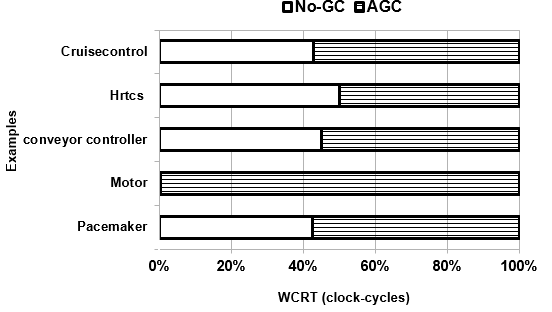
\includegraphics[scale=0.45]{wcetb.PNG}
    \label{fig:13a}
  }
  \subfloat[Statically analyzed method sizes for benchmarks]{
    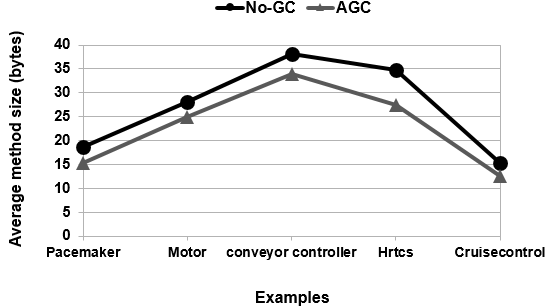
\includegraphics[scale=0.45]{msizeb.PNG}
    \label{fig:13b}
  }
  \caption{WCRT and method size comparison: No-GC vs. AGC}
  \label{fig:13}
\end{figure}

\section{Related Work and discussion}
\label{sec:related-work}

{\color{red}


  \subsection{Comparison with SCJ and RTSJ memory organization}
\label{sec:scj-rtsj}

\newsavebox{\reuse}
\begin{lrbox}{\reuse}
  \begin{minipage}[b]{0.7\linewidth}
    \begin{Verbatim}[numbers=right,commandchars=\\\[\]]
A a = null; \label[reuse:l1]
for (int i = 0; i< N; ++i) \label[reuse:l2]
 a = new A(); \label[reuse:l3]
emit S(a); \label[reuse:l4]
    \end{Verbatim}
  \end{minipage}
\end{lrbox}

We are not the first to advocate a GC-less approach for hard real-time
applications with memory managed languages, especially Java. There exist
previous works like the Safety Critical Java (SCJ)~\cite{scj2013}
specification, Ravenscar-Java~\cite{kwon2005ravenscar} and Real Time
Specification for Java (RTSJ)~\cite{bollella2000real} that present a
memory organization approach similar to the one presented in this
paper. SCJ, Ravenscar-Java and the RTSJ approaches divide the backing
store into multiple parts. A memory region called scoped memory is
allocated per real-time task (called a schedulable object in SCJ/RTSJ
terminology), which is automatically reclaimed, using pointer reset like
us, once the task completes execution. There also exists a permanent
memory area, called the immortal memory, similar to the permanent heap
advocated in this paper. Any object allocated in the immortal memory
lives throughout the lifetime of the application. One major difference
between the presented memory partitioning approach and the memory
partitioning in SCJ/Ravenscar-Java and RTSJ approaches is that in the
presented approach the same transient heap space (similar to scoped
memory in SCJ) can be shared by multiple synchronous parallel reactions,
whereas every single task gets allocated its own scoped memory (which
might be nested in another tasks scoped memory) in SCJ. This is because,
SCJ allows preemption of tasks during program execution, whereas in
SystemJ a clock-domain tick is atomic. RTSJ does allow access of scoped
memory by concurrent threads and only when the last thread exits the
scoped memory is the memory reclaimed.  Another important point of
differentiation is the reuse of memory words enabled by the proposed
approach. Consider the SystemJ code snippet in
Figure~\ref{fig:reuse}. An object \texttt{a}, of type \texttt{A} is
initialized multiple time on lines~\ref{reuse:l2}-\ref{reuse:l3}. The
proposed approach \textit{replaces} the \texttt{new} bytecode with
simple load instructions, hence, the object does \underline{not} get
allocated multiple times in the loop. In fact, the same memory location
(address/words) are reused by the proposed approach. In the SCJ/RTSJ
memory organization, every memory allocation bytecode (e.g.,
\texttt{new}) allocates new memory words and hence, reuse is
impossible. This is also the primary reason for the results shown in
Table~\ref{tab:1}.

\begin{figure}[h!]
  \centering
  \scalebox{0.7}{\usebox{\reuse}}
  \caption{SystemJ code snippet to show resue of memory words}
  \label{fig:reuse}
\end{figure}

Furthermore, in the proposed approach the compiler automatically decides
where to place the allocated objects, whereas in the SCJ and RTSJ
approaches, the programmer needs to explicitly and carefully allocate
objects to the correct memory areas manually. We believe that our
approach helps speed up development times.

The proposed algorithms also have a lot in common with a number of tools
proposed for easing development of programs in SCJ and RTSJ. The worst
case memory analyzer tool~\cite{andersen2013worst} developed for SCJ is
able to provide the maximum permanent memory and scoped memory sizes
needed for each task automatically, like us. But, the programmer is
still responsible for reserving the appropriate sized permanent memory
and scoped memory areas in the backing store. Compiler driven memory
allocation is a non-trivial task for SCJ and RTSJ applications, because
SCJ and RTSJ allow free use of the Java language, consequently bringing
all the disadvantages such as: pointer aliasing, shared memory
communication, etc, which we restrict in the SystemJ MoC. Finally, JVMs
other than JOP can be used to execute SystemJ programs with the proposed
memory organization, provided an array based backing store is available.

\subsection{Comparison with Real-time GC approaches}
\label{sec:rtgc}

Real-time garbage collectors (RTGCs) such as the ones proposed
in~\cite{gestegard2003time,kalibera2009scheduling} and the ones
presented in~\cite{pizlo2008study}, aim to achieve good garbage
collection throughput while providing analytic solutions to the worst
case execution times of a \textit{single} GC cycle. Once the GC cycle
times are obtained there is the need to schedule the GC work. The
scheduling can be either \textit{work} based; where the GC work is
performed at object allocation by the already present real-time tasks,
or \textit{time} based; where the GC runs as its own task and needs to
be scheduled with the other real-time tasks in the system. Both these
approaches suffer from drawbacks, such as determining the priority of
the GC task, etc~\cite{schoeberl2010scheduling}. The major drawback of
these approaches is that the equations capturing the GC cycle times
depend upon the memory allocation characteristic of the application. In
the general case, assuming the worst case memory allocation patterns
results in a very pessimistic GC worst case bound as shown
in~\cite{puffitsch2013design}. In this paper we are trying to remedy
this problem by removing the GC altogether.


\subsection{Limitations}
\label{sec:limitations}




}

% All one needs to provide is an array based backing store, which can be
% used to implement the memory organization for SystemJ as described in
% this paper. Finally, we would like to mention that the memory
% organization presented in this paper is applicable to JVMs other than
% JOP. All one needs to provide is an array based backing store, which
% can be used to implement the memory organization for SystemJ as
% described in this paper.

\section{Conclusion and future work}
\label{sec:concl-future-work}

In this paper we have presented a new memory organization and model for
hard real-time and safety-critical applications programmed in formal
synchronous languages with data support being provided by managed
language runtimes, primarily Java. % The presented approach takes a
% departure from the current practice of building new memory allocation
% and garbage collection algorithms that can meet at best soft real-time
% guarantees.
The presented approach utilizes the formal synchronous programming model
provided by SystemJ, to divide the Java objects into two types: (1)
transient objects, which are allocated for a single clock-domain
transition \textit{only} and are collected by simple pointer reset. (2)
Permanent objects, which are alive throughout the life time of the
application. Adhering to the synchronous model of computation, allows us
to perform compile time memory allocation, which means that our programs
are guaranteed to be free of execution time \mbox{\textit{out of
    memory}} exceptions. Furthermore, we are able to replace object
allocation bytecodes, with real-time analyzable alternatives, which
makes our approach amenable to non-pessimistic worst case execution time
analysis.

All the aforementioned qualitative improvements are further accompanied
by improvements in the program throughput (approximately $3\times$
faster memory allocation times) and worst case execution times, as
synchronization barriers necessary in real-time garbage collection
approaches become unnecessary in the proposed approach. Not to mention
the improvements in the number, size and compacted layout of allocated
Java objects and arrays.


% , and hence, preemptive and incremental garbage collection approaches
% have been the only solution to programming real-time systems with
% managed runtime environments to date. Preemptive scheduling generally
% leads to explosion in the number of states that need to be checked by
% automated formal verification tools, and hence, makes building safety
% critical systems hard, if not impossible. This proposal provides a
% solution to this problem.

% However, the proposed approach is not a penance. The proposed memory
% management technique, does indeed require the programmer to carefully
% design their real-time applications, as deep object copies need to be
% made explicitly by the programmer. Furthermore, 
We see opportunities for future optimization. Especially, relaxing the
object escapement restrictions currently enforced by the proposed
data-flow analysis. We also see an opportunity to \textit{reuse}
permanent heap memory allocations across clock-domain tick boundaries,
which we plan to address in the future.

% Bibliography
% \bibliographystyle{ACM-Reference-Format-Journals}
\bibliographystyle{wileyj}
\bibliography{main_bib}

% History dates
% \received{February 2007}{March 2009}{June 2009}

% Electronic Appendix
 % \elecappendix

\newpage
\medskip

% \section{This is an example of Appendix section head}

\section{Data-flow analysis pseudo-algorithms}
\label{ap:2}

Figure~\ref{fig:14} gives the pseudo-code implementing the data-flow
analysis algorithm for compile time memory allocation.

\newsavebox{\algone}
\begin{lrbox}{\algone}
  \begin{minipage}[b]{0.5\linewidth}
    \begin{algo}
      \SetKwData{Let}{let}
      \SetKwFunction{Steptwo}{Step2}
      \SetKwFunction{Reachable}{ReachableMethods}
      \SetKwFunction{Size}{sizeof}
      \KwIn{program: Program in RTL format} 
      \BlankLine
      \tcc*[h]{$pp$ is the set of program points}\\
      \Let \textbf{global} $pp \leftarrow \emptyset$\;\label{algone:l1}
      \Let $M \leftarrow$ \texttt{main}\;
      \Let $M \leftarrow$ \Reachable(\texttt{main}) $\cup$ $\{M\}$\;
      \Let $size \leftarrow$ \Size(signal class)\;
      \ForEach{$m \in M$} {
        \Let pp $\leftarrow$ ($size$, get in $m$, program points initializing signals)\;
      }
      \Steptwo(program,pp,\texttt{main})\;
    \end{algo}
  \end{minipage}
\end{lrbox}

\newsavebox{\algtwo}
\begin{lrbox}{\algtwo}
  \begin{minipage}[b]{0.5\linewidth}
    \begin{algo}
      \SetKwData{Let}{let}
      \SetKwFunction{Code}{code}
      \SetKwFunction{Signalset}{signalSet}
      \SetKwFunction{Emits}{emits}
      \SetKwFunction{InvokesMethod}{invokesMethod}
      \SetKwFunction{Steptwo}{Step2}
      \SetKwFunction{GetMethod}{getInvoked}
      \SetKwFunction{Stepthree}{Step3}
      \KwIn{program: Program in RTL format} 
      \KwIn{pp: Set of program points} 
      \KwIn{\texttt{method}: Method to scan for signal emissions} 
      \BlankLine
      \Let $S \leftarrow$ \Signalset(pp)\;
      \Let $C \leftarrow$ \Code(\texttt{method})\;
      \Let $PPC \leftarrow \emptyset$\;
      \ForEach{$c \in C$}{\label{algtwo:l1}
        \If{\Emits($c$,$S$)}{
          $PPC \leftarrow PPC\ \cup \{c\}$\;
        }
      }\label{algtwo:l2}
      \Stepthree(program,$PPC$,$C$)\;
      \ForEach{$c \in C$}{
        \If{\InvokesMethod($c$)}{
          \Steptwo(program,$c$,\GetMethod($c$))\;
        }
      }
    \end{algo}
  \end{minipage}
\end{lrbox}

\newsavebox{\algthree}
\begin{lrbox}{\algthree}
  \begin{minipage}[b]{0.5\linewidth}
    \begin{algo}
      \SetKwData{Let}{let}
      \SetKwFunction{Code}{code}
      \SetKwFunction{Signalset}{signalSet}
      \SetKwFunction{Emits}{emits}
      \SetKwFunction{GetExpr}{getExpr}
      \SetKwFunction{AffectsFields}{affectsFields}
      \SetKwFunction{AffectsVars}{affectsVars}
      \SetKwFunction{StepFour}{Step4}
      \SetKwFunction{StepFive}{Step5}
      \KwIn{program: Program in RTL format} 
      % \KwIn{pp: Set of program points} 
      \KwIn{$PPC$: Set of program points affected} 
      \KwIn{$C$: code of the method containing $PPC$}
      \BlankLine
      \ForEach{$ppc \in PPC$}{
        \uIf{\AffectsFields(\GetExpr($ppc$))}{
          \Let $pp \leftarrow pp\ \cup$ \StepFour(program,$ppc$,\GetExpr($ppc$),$C$)\;
        }
        \uElseIf{\AffectsVars(\GetExpr($ppc$))}{
          \Let $pp \leftarrow pp\ \cup$ \{\StepFive(program,$ppc$,\GetExpr($ppc$),$C$)\}\;
        }
        \lElse{\texttt{raise error}}
      }
    \end{algo}
  \end{minipage}
\end{lrbox}

\newsavebox{\algfour}
\begin{lrbox}{\algfour}
  \begin{minipage}[b]{0.5\linewidth}
    \begin{algo}
      \SetKwData{Let}{let}
      \SetKwFunction{Code}{code}
      \SetKwFunction{GetFields}{getFields}
      \SetKwFunction{Escape}{escape}
      \SetKwFunction{StepSix}{Step6}
      \SetKwFunction{FieldOf}{fieldOf}
      \SetKwFunction{HasRefFields}{hasRefFields}
      \SetKwFunction{GetAffectedFeilds}{getAffectedFields}
      \SetKwFunction{StepThree}{Step3}
      \SetKwFunction{Max}{max}
      \SetKwFunction{SizeOf}{sizeof}
      \KwIn{program: Program in RTL format} 
      \KwIn{$ppc$: Affected program point} 
      \KwIn{$pexpr$: Expression affecting field} 
      \KwIn{$C$: code of the method containing $ppc$} 
      \BlankLine
      \Let $f \leftarrow$ \FieldOf($pexr$)\;
      \Let ($size$,$defs$) $\leftarrow$ \StepSix(program,$ppc$,$f$,$C$)\;
      \lIf {$size \neq 0$} {\Return ($size$,$defs$)}\;
      \ForEach {$d \in defs$} { \label{step4:s}
        \uIf{!\Escape(program,$C$,$d$)} {
          \If {\HasRefFields($f$)} {
            % start2
            \Let $PPC \leftarrow$ \GetAffectedFeilds(\GetFields($f$))\;
            \StepThree(program,$PPC$,$C$)\;
          }
        }
        \lElse {
          \texttt{raise error}\;
        }
      }
      \Let $size \leftarrow$ \Max(\SizeOf($defs$))\; \label{step4:e}
      \Return ($size$,$defs$)\;
    \end{algo}
  \end{minipage}
\end{lrbox}

\newsavebox{\algfive}
\begin{lrbox}{\algfive}
  \begin{minipage}[b]{0.5\linewidth}
    \begin{algo}
      \SetKwData{Let}{let}
      \SetKwFunction{Code}{code}
      \SetKwFunction{GetFields}{getFields}
      \SetKwFunction{Escape}{escape}
      \SetKwFunction{StepSeven}{Step7}
      \SetKwFunction{VarOf}{varOf}
      \SetKwFunction{HasRefFields}{hasRefFields}
      \SetKwFunction{GetAffectedFields}{getAffectedFields}
      \SetKwFunction{StepThree}{Step3}
      \SetKwFunction{Max}{max}
      \SetKwFunction{SizeOf}{sizeof}
      \KwIn{program: Program in RTL format} 
      \KwIn{$ppc$: Affected program point} 
      \KwIn{$pexpr$: Expression affecting field} 
      \KwIn{$C$: code of the method containing $ppc$} 
      \BlankLine
      \Let $v \leftarrow$ \VarOf($pexr$)\;
      \Let $defs \leftarrow$ \StepSeven(program,$ppc$,$v$,$C$)\;
      \ForEach {$d \in defs$} {
        \uIf{!\Escape(program,$C$,$d$)} {
          \If {\HasRefFields($v$)} {\label{algfive:l1}
            % start2
            \Let $PPC \leftarrow$ \GetAffectedFields(\GetFields($v$))\;
            \StepThree(program,$PPC$,$C$)\;
          }\label{algfive:l2}
        }
        \lElse {
          \texttt{raise error}\;
        }
      }
      \Let $size \leftarrow$ \Max(\SizeOf($defs$))\;
      \Return ($size$,$defs$)\;
    \end{algo}
  \end{minipage}
\end{lrbox}

\newsavebox{\algsix}
\begin{lrbox}{\algsix}
  \begin{minipage}[b]{0.5\linewidth}
    \begin{algo}
      \SetKwData{Let}{let}
      \SetKwFunction{Escape}{escape}
      \SetKwFunction{ReachDef}{reachDef}
      \SetKwFunction{GetAllFields}{getAllFields}
      \SetKwFunction{GetCallers}{getCallers}
      \SetKwFunction{GetCallerPPC}{getCallerPPC}
      \SetKwFunction{GetVarSetting}{getVarSetting}
      \SetKwFunction{StepSeven}{Step7}
      \KwIn{program: Program in RTL format} 
      \KwIn{$ppc$: Affected program point} 
      \KwIn{$f$: Field affected} 
      \KwIn{$C$: code of the method containing $ppc$} 
      \BlankLine
      \Let $ofields \leftarrow$ \GetAllFields($C$) $\backslash$ \{$f$\} \;\label{algsix:l1}
      \Let $pcs \leftarrow$ \ReachDef($ppc$,$f$)\;
      \uIf {$pcs \neq \emptyset$} {
        \Let $defs \leftarrow \emptyset$\;
        \ForEach {$pc \in pcs$} {
          \Let $vf \leftarrow$ \GetVarSetting($f$,$pc$)\;
          \Let $tt \leftarrow$ \StepSeven(program,$pc$,$vf$,$C$)\;\label{algsix:s7c}
          \uIf {all other $field \in ofields$ have same $tt$} {
            \tcc*[h]{Concat in set $defs$}\\
            $defs \leftarrow defs\ \cup tt$\;
          }\lElse {
            \tcc*[h]{Append a new set in $defs$}\\
            $defs \leftarrow defs\ \cup \{tt\}$\;
          }
        }
        \Return (0,$defs$)\;
      }\label{algsix:l2}
      \Else {\label{algsix:l3}
        \tcc*[h]{Inter-procedural analysis}\\
        \tcc*[h]{Get all callers, including from GRC analysis}\\
        \Let $Callers \leftarrow$ \GetCallers($C$)\;
        \lIf {$Callers = \emptyset$} \texttt{raise Not\_init $f$}\;
        \Let $defs \leftarrow \emptyset$\;  
        \Let $sizes \leftarrow \emptyset$\;  
        \ForEach {$caller \in Callers$} {
          \Let $defs \leftarrow defs\ \cup$ \StepSix(program,\GetCallerPPC($C$),$f$,$caller$)\;
          \tcc*[h]{Similar to Figure~\ref{fig:8d}
            lines~\ref{step4:s}-\ref{step4:e}, to fill in the sizes set.}
        }
        \Let $size \leftarrow  max(sizes)$\;
        \Return ($size$,$defs$)\;
      }\label{algsix:l4}
    \end{algo}
  \end{minipage}
\end{lrbox}

\newsavebox{\algseven}
\begin{lrbox}{\algseven}
  \begin{minipage}[b]{0.5\linewidth}
    \begin{algo}
      \SetKwData{Let}{let}
      \SetKwFunction{Escape}{escape}
      \SetKwFunction{ReachDef}{reachDef}
      \SetKwFunction{NotReachable}{notReachable}
      \SetKwFunction{GetAllFields}{getAllFields}
      \SetKwFunction{GetExpr}{getExpr}
      \SetKwFunction{VarOf}{varOf}
      \SetKwFunction{GetVarSetting}{getVarSetting}
      \SetKwFunction{StepFour}{Step4}
      \KwIn{program: Program in RTL format} 
      \KwIn{$ppc$: Affected program point} 
      \KwIn{$v$: Variable affected} 
      \KwIn{$C$: code of the method containing $ppc$} 
      \BlankLine
      \Let $pcs \leftarrow$ \ReachDef($ppc$,$v$)\;\label{algseven:l1}
      \lIf{$pcs = \emptyset$} {\texttt{raise Not\_init}}\;\label{algseven:l3}
      \Let $defs \leftarrow \emptyset$\;
      \ForEach {$pc \in pcs$} {
        \uIf {\GetExpr($pc$) is \texttt{New} \textbf{or} \GetExpr($pc$) is \texttt{NewArray}} {
          $defs \leftarrow defs\ \cup \{pc\}$\;\label{algseven:l2} 
        }
        \uElseIf {\GetExpr($pc$) is \texttt{AffectField}} {
          \Let $expr \leftarrow$ \GetExpr($pc$)\;
          \Let (\_,$defs$) $\leftarrow$ \StepFour(program,$pc$,$expr$,$C$)\;
        }
        \uElseIf {\GetExpr($pc$) is \texttt{AffectVar}}{
          \Let $v \leftarrow$ \VarOf(\GetExpr($pc$))\;
          \Let (\_,$defs$) $\leftarrow$ \StepSeven(program,$pc$,$v$,$C$)\;\label{algseven:rec}
        }
        \Else {\label{algseven:l4}
          \tcc*[h]{Cannot handle new outside current method allocation}\\
          \texttt{raise Not\_handled}
        }\label{algseven:l5}
      }
      \tcc*[h]{Make sure that definitions are not reachable from each other}\\
      \If {$|defs| > 1$} {
        \textbf{assert}(\NotReachable($defs$))\;
      }
      \Return($defs$)\;
    \end{algo}
  \end{minipage}
\end{lrbox}

\begin{figure}[h!]
  \centering
  \subfloat[Step1:Scan signal initialization]{
    \scalebox{0.9}{\usebox{\algone}}
    \label{fig:8a}
  }
  \qquad
  \subfloat[Step2: Scan \texttt{setValue} method calls]{
    \scalebox{0.9}{\usebox{\algtwo}}
    \label{fig:8b}
  }
  \qquad
  \subfloat[Step3: For every affected field/variable get the object
  allocation program points]{
    \scalebox{0.9}{\usebox{\algthree}}
    \label{fig:8c}
  }
  \qquad
  \subfloat[Step4: Get object allocation program points for affected field]{
    \scalebox{0.9}{\usebox{\algfour}}
    \label{fig:8d}
  }
  \caption{Data-flow analysis pseudo-algorithm}
  \label{fig:14}
\end{figure}

\begin{figure}
  \centering
  \ContinuedFloat
  \subfloat[Step5: Get object allocation program points for affected variables]{
    \scalebox{0.9}{\usebox{\algfive}}
    \label{fig:8e}
  }
  \qquad
  \subfloat[Step6: Search object allocation program points for affected field]{
    \scalebox{0.9}{\usebox{\algsix}}
    \label{fig:8f}
  }
  \subfloat[Step7: Search object allocation point(s) for method local affected
  variable]{
    \scalebox{0.9}{\usebox{\algseven}}
    \label{fig:8g}
  }
  \qquad
  \caption{Data-flow analysis pseudo-algorithm}
  \label{fig:14}
\end{figure}


\section{The GRC analysis algorithm} \label{ap:1}

\begin{algorithm}[t!]
	\DontPrintSemicolon
	\SetKw{Let}{let}
	\SetKw{Fn}{Function}
	\SetAlgoNoEnd
	\SetKwFunction{KwCol}{collect\_cd\_nodes}
	\SetKwFunction{KwCrNode}{create\_node}
	\SetKwFunction{KwFindFork}{find\_matching\_fork}
	\KwIn{$GRC$ : $(V,E)$}
	\KwOut{$mList$: a set of set of $mNode$}
	\KwData{$V_{cd}$: a set of set of clock-domain nodes}
	\KwData{$mNode$ = [$Name$:string,$Must$:$mNode$,$May$:set of $mNode$] }
	\tcc{Grouping nodes for each clock-domain}
	\Let{$V_r = \emptyset \cup V$}\;
	\Let{$V_{cd} = \emptyset$}\;
	\ForEach{$v \in V$}{
		\lForEach{$(v_i,v_j) \in E$}{\lIf{$v_j = v$}{$V_r = V_r \backslash \{v\}$}}
	}
	\lForEach{$v \in V_r$}{$V_{cd} = V_{cd} \cup$ \{\KwCol{$v,E$}\}}\;
	\tcc{Perform May and Must analysis}
	\ForAll{$V \in V_{cd}$}{
		\Let $V_{temp} = \emptyset$\;
		\ForEach{$v \in V$}{
			$V_{temp} = V_{temp} \cup$ \{\KwCrNode{$v,E$}\}
		}
		$mList = mList \cup \{V_{temp}\}$
	}
	\;
	\Fn \KwCrNode{$v,E$}:\;
	\Begin{
		\Let{$E_i = \lambda(v)$}\;
		\If{$v = ActionNode$}{
			\If{$|E_i| = 1$}{
				\Let{$\{(v_i,v_j)\} = E_i$}\;
				\Let $newNode = [Name \leftarrow get\_name(v_j); Must
				\leftarrow \KwCrNode{$v_i,E$}; May \leftarrow Null]$\;
				\Return{newNode}
			}
			\ElseIf{$|E_i| > 1$}{
				\Let $V_{temp} = \emptyset$\;
				\ForEach{$(v_i,v_j) \in E_i$}{
					$V_{temp} = V_{temp} \cup \{\KwCrNode{$v_i,E$}\}$
				}
				\Return{$[Name \leftarrow get\_name(v_j); Must
				\leftarrow Null ; May \leftarrow V_{temp}]$}
			}
			\ElseIf{$|E_i| = 0 $}{
				\Return{$[Name \leftarrow get\_name(v_j); Must
				\leftarrow Null; May \leftarrow Null]$}
			}
		}
		\ElseIf{$v =JoinNode$}{
			\Let{$v = $ \KwFindFork{$v$}}\;
			\Let{$\{(v_i,v_j)\} = \lambda(v)$}\;
			\Return{\KwCrNode{$v_i,E$}}
		}
		\Else{
			\If{$|E_i| = 0$}{\Return{Null}}
			\ElseIf{$|E_i| = 1$}{\Return{\KwCrNode{$v_i,E$}}}
		}
	}
	\;
	\Fn \KwCol{$v,E$}:\;
	\Begin{
		\Let $V_{temp} = \emptyset$\;
		\ForEach{$(v_i,v_j) \in E$}{\If{$v = v_i$}{
			$V_{temp} = V_{temp} \cup \{v_j\}$\;
			$V_{temp} = V_{temp} \cup$ \KwCol{$v_j,E$}
		}}
		\Return{$V_{temp}$}
	}
	\caption{May and Must analysis}
	\label{alg:agrc}
	
\end{algorithm}

The algorithm for obtaining \textit{may} and \textit{must} relationships
between the GRC nodes is shown in Algorithm~\ref{alg:agrc}. The input to
this algorithm is an GRC, which is a tuple $(V,E)$ as explained
previously. The first part of the algorithm, lines 1-5, groups all the
nodes, which are belonging to the same clock-domain. For instance, lines
3-4 initializes a set $V_r$, which consists of a root node of all
clock-domains in GRC. The algorithm then traverses every clock-domain
graph, starting from these root nodes via a recursive function
\texttt{collect\_cd\_nodes($v,E$)} (line 5). A result is a set of set of
GRC nodes $V_{cd}$. Next \textit{May} and \textit{Must} analysis is
performed (lines 6-10). Every node in $V_{cd}$ is given as an input to
the function \texttt{create\_node($v,E$)} (line 9), which traverses the
graph backward starting from the input until it reaches the root node.
Function \texttt{create\_node} first maps the input node to a set of
edges $E_i$ using the lambda function (line 14). It is then divided into
three parts:

\begin{enumerate}

\item If the current node type is an \texttt{JDN} node (line 15) and

  \begin{enumerate}

  \item the number of element in $E_i$ is 1, then the only
    parent node $v_i$ \textit{must} be called before
    $v_j$. Then a new node of type $mNode$ is created with
    its field $Must$ initialized to the result of
    recursive call of \texttt{create\_note}.

  \item the number of element in $E_i$ is greater than 1,
    then any parent nodes $v_i \in E_i$ \textit{may} be
    called before $v_j$.  A set of $mList$, consisting
    return results of \texttt{create\_node} of each parent
    node $v_i \in E_i$, is assigned to the field $May$ of
    a newly created $mNode$.

  \item the number of element in $E_i$ is 0, then a new
    $mNode$ is created with both its $Must$ and $May$
    fields initialized to $Null$.

  \end{enumerate}

\item If the current node type is \texttt{Join}, this
  means that there are two or more parallel reactions
  forked at the \texttt{Fork} node, which \textit{must} be
  found in one of the recursive parents of the current
  node. Hence, the algorithm must continue the backward
  traversal from this \texttt{Fork} node. During
  compilation, the compiler has already constructed a
  Hashtable which maps each \texttt{Join} node to its
  corresponding \texttt{Fork} node as shown in line 28.

\item If the current node type is other than \texttt{JDN}
  (line 31) and

  \begin{enumerate}

  \item the number of parent node ($|E_i|$) is 0 , then
    \textit{Null} is returned

  \item the number of parent node is 1, then a result of
    \texttt{create\_node} is returned.

  \end{enumerate}

\end{enumerate}



\end{document}
% End of v2-acmsmall-sample.tex (March 2012) - Gerry Murray, ACM


